\documentclass[11pt,a4paper]{article}
\usepackage[utf8]{inputenc}
\usepackage[T1]{fontenc}
\usepackage{lmodern}
\usepackage[a4paper,margin=1in]{geometry}
\usepackage{amsmath,amssymb,amsfonts,amsthm}
\usepackage{graphicx}
\usepackage{tikz}
\usetikzlibrary{arrows.meta, positioning, decorations.pathmorphing, shapes.geometric}
\usepackage{booktabs}
\usepackage{tabularx}
\usepackage{longtable}
\usepackage{array}
\usepackage{enumitem}
\usepackage{float}
\usepackage{appendix}
\usepackage{physics}
\usepackage{hyperref}
\hypersetup{colorlinks=true, linkcolor=black, citecolor=black, urlcolor=black}
\usepackage{cleveref}

\graphicspath{{figures/}}

\linespread{1.12}
\setlength{\parskip}{0.3em}

% Academic theorem environments (black and white, no colour)
\theoremstyle{plain}
\newtheorem{proposition}{Proposition}[section]
\newtheorem{conjecture}{Conjecture}[section]
\theoremstyle{definition}
\newtheorem{definition}{Definition}[section]
\newtheorem{example}{Example}[section]
\theoremstyle{remark}
\newtheorem{remark}{Remark}[section]

\newcommand{\ee}{\mathrm{e}}
\newcommand{\ii}{\mathrm{i}}
\newcommand{\kB}{k_{\mathrm{B}}}
\newcommand{\calL}{\mathcal{L}}
\newcommand{\calK}{\mathcal{K}}
\newcommand{\calP}{\mathcal{P}}
\newcommand{\calQ}{\mathcal{Q}}
\newcommand{\calH}{\mathcal{H}}
\newcommand{\calC}{\mathcal{C}}
\newcommand{\calM}{\mathcal{M}}
\newcommand{\calR}{\mathcal{R}}
\newcommand{\calA}{\mathcal{A}}
\newcommand{\bbR}{\mathbb{R}}
\newcommand{\bbC}{\mathbb{C}}
\newcommand{\bbZ}{\mathbb{Z}}
\newcommand{\gz}{g_z}
% additional macros (several are needed by Abhishek's part, kept intact)
\newcommand{\calI}{\mathcal{I}}
\newcommand{\calD}{\mathcal{D}}
\newcommand{\calS}{\mathcal{S}}
\newcommand{\calB}{\mathcal{B}}
\newcommand{\bbN}{\mathbb{N}}
\newcommand{\expect}[1]{\langle #1 \rangle}
\renewcommand{\d}{\mathrm{d}}
\renewcommand{\dd}{\mathrm{d}}

\title{\bfseries Thermodynamic Quantum Logic Gates:\\
From the Autonomous Neuron to Floquet--Buffered\\
Non--Markovian Operation}
\author{Sparsho Chakraborty \and Abhishek}
\date{\today}

\begin{document}
\maketitle

\begin{abstract}
\noindent
This document consolidates the theory, derivations, numerical
reconstructions, non--Markovian tensor--network formulation, and Floquet
buffer architecture developed for the thermodynamic--neuron project into
a single reference. Part~\ref{part:sparsho} (Sparsho) is a self--contained,
build--up derivation: it starts from a single qubit in a heat bath,
constructs the open--system master equation and shows explicitly how the
system--bath interaction is absorbed into the dissipator, introduces the
reset model, builds the virtual qubit and the resonant three--body
interaction, assembles the autonomous NOT gate and the general
linearly--separable neuron, reproduces the baseline logic numerically,
and then extends the treatment beyond weak coupling through the
Nakajima--Zwanzig equation, the influence functional, and process--tensor
(PT--MPO/TEMPO) methods, culminating in the Floquet--buffer architecture
and its robustness analysis. All approximations are collected in a single
table (Table~\ref{tab:approximations}). Part~\ref{part:abhishek}
(Abhishek) contains the rigorous periodically--driven open--system
formulation, kept intact.
\end{abstract}

\tableofcontents
\clearpage

% #####################################################################
\part{Sparsho: From the Single Qubit to Floquet--Buffered Thermodynamic Logic}
\label{part:sparsho}
% #####################################################################

\section{Introduction: thermodynamics of computation}
\label{sec:intro}
Thermodynamic computing studies the energetic and entropic cost of
information processing, and asks whether physical relaxation can be used
\emph{directly} as a computational resource. In ordinary digital logic,
robustness is obtained by engineering large barriers between stable
states and by externally clocking transistor networks. In autonomous
quantum thermal machines the situation is reversed: computation is
performed by relaxation itself. Logical inputs are encoded into
thermodynamic parameters (the inverse temperatures of heat baths), heat
currents process those inputs, and the final state of an output degree of
freedom is decoded as a logical value. This viewpoint continues the
thermodynamics--of--information tradition of Landauer and Bennett and the
quantum thermal--machine programme in which autonomous devices and
\emph{virtual temperatures} are operational resources.

The appeal of the autonomous model is that it needs no pre--programmed
sequence of unitary gates. Its fragility is that the usual thermodynamic
accounting depends on three conditions: weak system--bath coupling, rapid
decay of bath correlations, and a clean separation between system
timescales and reservoir memory. This part builds the model from the
ground up so that every one of those conditions is visible and labelled
(they are collected in Table~\ref{tab:approximations}), reproduces the
baseline logic numerically, and then asks what must change when the
conditions fail --- which is precisely where the Floquet buffer and the
non--Markovian machinery enter.

\paragraph{Scope of Part~\ref{part:sparsho}.} Sections
\ref{sec:single-qubit}--\ref{sec:machine} build the open--system tools;
Sections \ref{sec:virtual}--\ref{sec:general} build the neuron;
Section~\ref{sec:reconstruction} reproduces the baseline logic
numerically; Sections \ref{sec:nonmarkov}--\ref{sec:floquet} extend the
treatment beyond weak coupling and introduce the Floquet buffer; and
Section~\ref{sec:robustness} presents the robustness programme.
Part~\ref{part:abhishek} then gives the rigorous driven--dissipative
formulation.

\subsection*{Derivation map for the supervisor}
\addcontentsline{toc}{subsection}{Derivation map for the supervisor}
The document is intentionally written as a derivation trail rather than
as a short paper.  The following map states what each major block proves,
where the physical idea enters, and why the step is needed.
\begin{center}
\small
\begin{tabularx}{\textwidth}{@{}l X X@{}}
\toprule
Block & What is derived & Why it is needed \\
\midrule
Single qubit &
The Gibbs state $\tau(\beta)$ and the population
$g(\beta\epsilon)=1/(1+\ee^{\beta\epsilon})$. &
This is the thermal sigmoid from which the neuron activation function
ultimately comes. \\
Open system derivation &
The system--bath Hamiltonian is projected to a reduced master equation;
the interaction $H_{SB}$ becomes rates, jumps, Lamb shifts, and memory
kernels. &
This answers where the bath Hamiltonian and interaction have gone in the
effective equations. \\
Reset model &
The reset dissipator, heat current, entropy production, and the precise
approximations that make them thermodynamically consistent. &
This is the Markovian computational baseline used in the original
thermodynamic neuron. \\
Virtual qubit &
The two machine qubits define an effective transition with inverse
temperature $\beta_v=(\beta_1\epsilon_1-\beta_0\epsilon_0)/\epsilon_z$. &
The input bath temperature is converted into an effective output bias. \\
Collector and modulator &
Energy--conserving three--body swapping gives collector current; the
modulator competes with it and fixes a stable output point. &
The collector alone is only an amplifier; the modulator turns it into a
gate with a threshold and noise margin. \\
Perceptron mapping &
The general virtual temperature is a linear score in the input inverse
temperatures, followed by a thermal sigmoid. &
This explains why a single thermodynamic neuron realizes exactly
linearly separable Boolean functions. \\
Non--Markovian extension &
The Nakajima--Zwanzig memory kernel, influence functional, PT--MPO/TEMPO
discretization, and convergence checks. &
This shows what must replace the local Lindblad/reset picture when bath
memory is important. \\
Floquet buffer &
A periodically driven intermediate subsystem produces sidebands,
spectral filtering, and stroboscopic control. &
This is the proposed mechanism for reducing leakage and improving
logical distinguishability. \\
\bottomrule
\end{tabularx}
\end{center}

\section{The single qubit}
\label{sec:single-qubit}
A qubit is a two--level system with Hilbert space $\calH=\bbC^2$, basis
$\{\ket{0},\ket{1}\}$, and free Hamiltonian
\begin{equation}
H = E_0\ket{0}\bra{0}+E_1\ket{1}\bra{1}
\;\xrightarrow{\;E_0:=0\;}\;
H=\epsilon\,n,\qquad n:=\ket{1}\bra{1},\quad \epsilon:=E_1-E_0,
\label{eq:H-single}
\end{equation}
where only the gap $\epsilon$ is physical (the zero of energy is set at
the ground state). In contact with a bath at inverse temperature
$\beta=1/\kB T$ the qubit relaxes to the Gibbs state
\begin{equation}
\tau(\beta)=\frac{\ee^{-\beta H}}{Z},\quad Z=1+\ee^{-\beta\epsilon},
\qquad
\tau(\beta)=\frac{\ket{0}\bra{0}+\ee^{-\beta\epsilon}\ket{1}\bra{1}}
{1+\ee^{-\beta\epsilon}} .
\label{eq:gibbs}
\end{equation}
The excited--state occupation is the Fermi--Dirac function, which is
simultaneously the logistic sigmoid,
\begin{equation}
\boxed{\;
g(\beta\epsilon):=\bra{1}\tau(\beta)\ket{1}
=\frac{1}{1+\ee^{\beta\epsilon}} = f(\beta\epsilon),\qquad
f(x):=\frac{1}{1+\ee^{x}} .\;}
\label{eq:fermi}
\end{equation}
This single identity --- a thermal population is a sigmoid of an inverse
temperature --- is the seed of the entire neuron--perceptron
correspondence developed in Section~\ref{sec:general}. The
detailed--balance ratio that every thermalization model must reproduce
is
\begin{equation}
\frac{\bra{1}\tau(\beta)\ket{1}}{\bra{0}\tau(\beta)\ket{0}}
=\ee^{-\beta\epsilon}.
\label{eq:db-ratio}
\end{equation}

\section{Open quantum systems: where the bath Hamiltonian goes}
\label{sec:open}
This section resolves a point that is easy to miss in the working
equations: if the qubit is coupled to a bath, \emph{where is the
qubit--bath interaction Hamiltonian, and why does it not appear
explicitly in the master equation?} The answer is that it is present
microscopically but, after the bath is eliminated, it is \emph{converted}
into the dissipator. We show this in the projection--operator
(Nakajima--Zwanzig) language, which also exposes exactly where the
Markovian description can fail --- the entry point for
Section~\ref{sec:nonmarkov}.

\subsection{A closed qubit cannot thermalize}
Unitary evolution $\rho(t)=\ee^{-\ii Ht}\rho(0)\ee^{\ii Ht}$ of the qubit
\eqref{eq:H-single} generates only phases; the populations
$\bra{0}\rho\ket{0},\bra{1}\rho\ket{1}$ are constant. A closed qubit
therefore cannot relax to \eqref{eq:gibbs}. Dissipation, and hence
computation--by--relaxation, is impossible without an environment: the
bath is the only object that can change populations and drive the system
to a steady state.

\subsection{Microscopic model}
Restore the environment as a bosonic reservoir bilinearly and
transversally coupled to the qubit,
\begin{equation}
H_{\mathrm{tot}} = \underbrace{H_S}_{\epsilon\,n}
+ \underbrace{H_B}_{\sum_k\omega_k a_k^\dagger a_k}
+ \underbrace{H_{SB}}_{\sigma_x\otimes\sum_k\lambda_k(a_k+a_k^\dagger)} .
\label{eq:Htot-open}
\end{equation}
The coupling is transverse ($\sigma_x=\sigma_++\sigma_-$) because the bath
must be able to \emph{flip} the qubit to exchange the quantum $\epsilon$;
a longitudinal $\sigma_z$ coupling would only dephase and never thermalize
(a fact we exploit deliberately when the Floquet drive is chosen
longitudinal in Section~\ref{sec:floquet}). The bilinearity is
approximation (A2) in Table~\ref{tab:approximations}.

\subsection{Nakajima--Zwanzig equation and the origin of memory}
\label{sec:NZ}
Write the exact Liouville--von~Neumann equation
$\dot\rho_{\mathrm{tot}}=\calL\rho_{\mathrm{tot}}$,
$\calL(\cdot)=-\ii[H_{\mathrm{tot}},\cdot]$, and introduce the projection
superoperators onto a reference bath state $\rho_B$,
\begin{equation}
\calP X = \Tr_B(X)\otimes\rho_B,\qquad \calQ=1-\calP .
\end{equation}
Projecting the exact equation and formally solving the $\calQ$ part gives
the exact Nakajima--Zwanzig equation for the relevant part
$\calP\rho_{\mathrm{tot}}$,
\begin{align}
\frac{\dd}{\dd t}\calP\rho_{\mathrm{tot}}(t)
&= \calP\calL\calP\rho_{\mathrm{tot}}(t)
+ \int_0^t \calK(t-\tau)\,\calP\rho_{\mathrm{tot}}(\tau)\,\dd\tau
+ \calI(t),
\label{eq:NZ}\\
\calK(t-\tau) &= \calP\calL\calQ\,\ee^{\calQ\calL(t-\tau)}\,\calQ\calL\calP,
\qquad
\calI(t)=\calP\calL\calQ\,\ee^{\calQ\calL t}\,\calQ\rho_{\mathrm{tot}}(0).
\end{align}
For a factorized initial state $\calQ\rho_{\mathrm{tot}}(0)=0$, so
$\calI(t)=0$ (this is approximation (A1)). The memory kernel $\calK$ is
the mathematical origin of non--Markovianity: the present reduced motion
depends on the system's history. Equation~\eqref{eq:NZ} is exact; the
Markovian master equation is what remains after three further
approximations.

\subsection{Born--Markov--secular reduction and the dissipator}
\label{sec:BMS}
Passing to the interaction picture, integrating once, tracing out the
bath (using $\Tr_B[B_a\rho_B]=0$), and applying in turn the Born (A2),
Markov (A3) and secular (A4) approximations yields the
Gorini--Kossakowski--Sudarshan--Lindblad (GKSL) master equation
\begin{equation}
\boxed{\;
\dot\rho_S = -\ii[H_S+H_{\mathrm{LS}},\rho_S]
+ \sum_\omega \gamma(\omega)\!\left[A(\omega)\rho_S A^\dagger(\omega)
-\tfrac12\{A^\dagger(\omega)A(\omega),\rho_S\}\right],
\;}
\label{eq:GKSL}
\end{equation}
with eigenoperators $A(\omega)$ of $H_S$ (for the qubit,
$A(\pm\epsilon)=\sigma_\mp$), rates
$\gamma(\omega)=\int_{-\infty}^\infty \ee^{\ii\omega t}C(t)\,\dd t$ set by
the bath correlation function $C(t)=\Tr_B[\tilde B(t)B\rho_B]$, and a Lamb
shift $H_{\mathrm{LS}}$ that merely renormalizes $\epsilon$. For the qubit
this is
\begin{equation}
\dot\rho = -\ii[H_S,\rho]
+\gamma_\downarrow\big(\sigma_-\rho\sigma_+-\tfrac12\{\sigma_+\sigma_-,\rho\}\big)
+\gamma_\uparrow\big(\sigma_+\rho\sigma_--\tfrac12\{\sigma_-\sigma_+,\rho\}\big).
\label{eq:GKSL-qubit}
\end{equation}
\emph{This is the answer to the question posed above.} The interaction
Hamiltonian $H_{SB}=\sigma_x\otimes B$ no longer appears as a
Hamiltonian: eliminating the bath has converted it into the two
dissipative channels of \eqref{eq:GKSL-qubit} --- $\gamma_\downarrow$
multiplying $\sigma_-$ (emission), $\gamma_\uparrow$ multiplying
$\sigma_+$ (absorption). The bath Hamiltonian $H_B$ has disappeared
entirely; the coupling survives only through the two rates. That is why
the working equations carry a free Hamiltonian and a dissipator but no
explicit qubit--bath interaction Hamiltonian.

The two rates are locked by the Kubo--Martin--Schwinger (detailed
balance) condition $\gamma(-\omega)=\ee^{-\beta\omega}\gamma(\omega)$, so
\begin{equation}
\frac{\gamma_\uparrow}{\gamma_\downarrow}=\ee^{-\beta\epsilon},
\qquad\Rightarrow\qquad
p_{\mathrm{ss}}=\frac{\gamma_\uparrow}{\gamma_\uparrow+\gamma_\downarrow}
= g(\beta\epsilon),
\label{eq:db-rates}
\end{equation}
i.e.\ the qubit relaxes to exactly the thermal population \eqref{eq:fermi}.

\subsection{The reset model}
\label{sec:reset}
Since only populations matter for the logic, we adopt the simplest
dissipator with the correct fixed point --- the reset (collisional)
model (A5),
\begin{equation}
\calL^{(k)}[\rho]=\gamma_k\big(\Tr_k[\rho]\otimes\tau(\beta_k)-\rho\big),
\label{eq:reset}
\end{equation}
in which qubit $k$ is, with rate $\gamma_k$, swapped for a fresh bath
qubit in the thermal state $\tau(\beta_k)$. It manifestly satisfies local
detailed balance $\calL^{(k)}[\tau(\beta_k)]=0$. The heat current into
bath $k$ is
\begin{equation}
j_k:=\Tr\!\big[H\calL^{(k)}[\rho]\big]
=\gamma_k\epsilon_k\big[g(\beta_k\epsilon_k)-p_k\big],
\label{eq:current-reset}
\end{equation}
with $p_k$ the excited population of qubit $k$. A qubit coupled to two
baths acquires the sum of two dissipators, and the total current is the
sum.

\subsection{Multi--qubit machines, currents, entropy production}
\label{sec:machine}
A machine of qubits $\{C_k\}$ has free Hamiltonian
$H_0=\sum_k\epsilon_k n_k$ and a time--independent, energy--preserving
interaction $H_{\mathrm{int}}$ with $[H_{\mathrm{int}},H_0]=0$ (A6): the
interaction may only connect degenerate eigenstates of $H_0$, shuffling
excitations without changing the bare energy. Under weak coupling the
machine obeys the local master equation (A7)
\begin{equation}
\dot\rho=-\ii[H_0+H_{\mathrm{int}},\rho]+\sum_k\calL^{(k)}[\rho].
\label{eq:local-me}
\end{equation}
The second law for this class of machines is
\begin{equation}
\dot\Sigma:=\dot S(\rho)-\sum_k\beta_k j_k \ge 0,\qquad
S(\rho)=-\Tr[\rho\ln\rho],
\label{eq:entropy-prod}
\end{equation}
and in a nonequilibrium steady state ($\dot S=0$) all produced entropy is
the weighted heat dumped into the baths, $\dot\Sigma=-\sum_k\beta_k j_k$.
This $\dot\Sigma$ is the ``dissipation'' whose trade--off against
accuracy we quantify in Section~\ref{sec:notgate}. The heat/work split
that defines $j_k$ is itself an approximation (A11) that becomes
ambiguous at strong coupling --- the caveat that Sections
\ref{sec:nonmarkov}--\ref{sec:robustness} take seriously.

% ---------------------------------------------------------------------
\begin{table}[t]
\centering\small
\caption{Master list of approximations used in Part~\ref{part:sparsho},
with the replacement each makes, its regime of validity, and the failure
mode when it is violated. Tags are referenced throughout the text.}
\label{tab:approximations}
\begin{tabularx}{\textwidth}{@{}l l X X@{}}
\toprule
Tag & Approximation & Statement / replacement & Regime of validity \& failure mode \\
\midrule
(A1) & Factorized initial state &
$\rho_{\mathrm{tot}}(0)=\rho_S(0)\otimes\rho_B$, so $\calI(t)=0$ in
\eqref{eq:NZ} &
Valid if system and bath start uncorrelated; else an inhomogeneous
memory term appears. \\
(A2) & Born / weak coupling &
$\rho_{\mathrm{tot}}(t)\approx\rho_S(t)\otimes\rho_B$; $H_{SB}$ bilinear &
$\lambda\ll\epsilon$; fails when bath back--action and interaction energy
are non--negligible. \\
(A3) & Markov / short memory &
$\rho_S(\tau)\to\rho_S(t)$, $\int_0^t\to\int_0^\infty$ &
$\tau_B\ll\tau_R$; fails for structured reservoirs that return
information (backflow). \\
(A4) & Secular / RWA &
drop terms with $\omega\neq\omega'$ &
$\gamma\ll$ Bohr gaps; fails for near--degenerate transitions and drive
sidebands. \\
(A5) & Reset thermalization &
$\calL^{(k)}\rho=\gamma_k(\Tr_k\rho\otimes\tau(\beta_k)-\rho)$ &
Steady--state populations only; changes transient shape, not the
inversion mechanism. \\
(A6) & Energy--preserving $H_{\mathrm{int}}$ &
$[H_{\mathrm{int}},H_0]=0$ &
$\chi\ll\epsilon$; off--resonant (energy--changing) terms otherwise leak. \\
(A7) & Local master equation &
bare--qubit dissipators in \eqref{eq:local-me} &
$\chi\ll\epsilon$; else use the global (dressed) dissipator to avoid
second--law violations. \\
(A8) & Modulator pinned to reference &
$p_\calM^{\mathrm{ss}}\approx\gz(\beta_r)$ &
$\mu'\ll\gamma$; else the modulator is dragged by the output bath. \\
(A9) & Adiabatic elimination &
steady currents inserted into the slow $\beta_z$ ODE &
$\mu,\mu'\ll\gamma$; error $O(\mu/\gamma)$; fails if timescales overlap. \\
(A10) & Small--$\epsilon_z$ sigmoid &
$\gz(\beta)\approx\tfrac12-\tfrac{\beta\epsilon_z}{4}$ &
$\epsilon_z\ll\epsilon_1$; larger $\epsilon_z$ blurs the parameter roles. \\
(A11) & Weak heat--current split &
$\dot Q_\alpha=\Tr(H_S\mathcal D_\alpha\rho)$ &
Weak coupling; reduced--system heat currents ambiguous at strong
coupling. \\
(A12) & Spin-chain bath proxy &
Each chain site has $d=2$ instead of a converged bosonic cutoff &
Tests tensor geometry and entanglement compression, not a quantitative
bosonic reservoir. \\
(A13) & Finite graph/time window &
$L\leq4$ and $0\leq t\leq4$ in the exact graph benchmark &
Valid before boundary reflections dominate; does not establish a
periodic or thermodynamic steady state. \\
(A14) & Schmidt truncation &
Retain the smallest $\chi$ with discarded weight at most $10^{-10}$ &
Controlled state-compression criterion; observables still require a
separate convergence test in $\chi$. \\
\bottomrule
\end{tabularx}
\end{table}

\section{The virtual qubit and the resonant interaction}
\label{sec:virtual}

\subsection{Virtual qubit and virtual temperature}
Take two qubits $C_0,C_1$ (gaps $\epsilon_0\ge\epsilon_1$) each in their
own bath at $\beta_0,\beta_1$. Absent interaction the joint state is the
product $\tau_{C_0}(\beta_0)\otimes\tau_{C_1}(\beta_1)$. The two crossed
states
\begin{equation}
\ket{0}_v:=\ket{0}_{C_0}\ket{1}_{C_1},\qquad
\ket{1}_v:=\ket{1}_{C_0}\ket{0}_{C_1}
\end{equation}
span a \emph{virtual qubit} of gap $\epsilon_v=\epsilon_0-\epsilon_1$.
Its population ratio defines a \emph{virtual temperature} exactly as in
\eqref{eq:db-ratio}:
\begin{equation}
\ee^{-\beta_v\epsilon_v}
=\frac{P_{10}}{P_{01}}
=\frac{\ee^{-\beta_0\epsilon_0}}{\ee^{-\beta_1\epsilon_1}}
\;\Rightarrow\;
\boxed{\;\beta_v=\frac{\epsilon_0}{\epsilon_0-\epsilon_1}\beta_0
-\frac{\epsilon_1}{\epsilon_0-\epsilon_1}\beta_1 .\;}
\label{eq:betav}
\end{equation}
The virtual inverse temperature is a \emph{linear combination of the
input inverse temperatures} --- the perceptron weighted sum. It can lie
outside $[\beta_0,\beta_1]$ and even go negative (population inversion),
giving the refrigerator / heat--pump / heat--engine regimes as $\beta_1$
is swept at fixed $\beta_0$.

\subsection{The resonant three--body interaction}
\label{sec:interaction}
Add a target qubit $C_z$ intended to inherit $\beta_v$. For a weak,
energy--preserving coupling to transfer excitations resonantly between
the virtual qubit and $C_z$, choose
\begin{equation}
\boxed{\;\epsilon_z=\epsilon_v=\epsilon_0-\epsilon_1,\;}
\label{eq:resonance}
\end{equation}
which makes $\ket{100}$ (energy $\epsilon_0$) and $\ket{011}$ (energy
$\epsilon_1+\epsilon_z$) degenerate. The unique Hermitian, energy--
preserving operator connecting only this pair is the three--body swap
\begin{equation}
\boxed{\;
H_{\mathrm{int}}
=\chi\big(\ket{100}\bra{011}+\ket{011}\bra{100}\big)
=\chi\big(\sigma_+^{(0)}\sigma_-^{(1)}\sigma_-^{(z)}+\mathrm{h.c.}\big),
\;}
\label{eq:Hint}
\end{equation}
with ordering $(C_0C_1C_z)$. In virtual--qubit variables
$H_{\mathrm{int}}=\chi(\ket{1}_v\ket{0}_{C_z}\bra{0}_v\bra{1}_{C_z}
+\mathrm{h.c.})$: a resonant swap between the virtual qubit and $C_z$.
Five points fix its form.
\begin{enumerate}[label=(\roman*),leftmargin=*]
\item \emph{Energy conservation / RWA.} Under \eqref{eq:resonance},
$\ket{100}$ and $\ket{011}$ are the only degenerate pair differing by an
allowed excitation rearrangement; every other off--diagonal term changes
the bare energy and is dropped by the rotating--wave argument (A6).
\item \emph{Three--body, not pairwise.} The virtual qubit is a joint
property of $C_0,C_1$; a two--body $\sigma_+^{(0)}\sigma_-^{(1)}$ only
rotates the excitation between them and transfers nothing to $C_z$.
\item \emph{Physical action.} The swap places the virtual qubit in
thermal contact with $C_z$, so in steady state $C_z$ carries $\beta_v$.
\item \emph{Dropped partners.} Terms creating three excitations oscillate
at $\epsilon_0+\epsilon_1+\epsilon_z$ and average away with error
$O(\chi/\epsilon)$.
\item \emph{No bare $C_0$--$C_1$ or $\sigma_z\sigma_z$ coupling.} These
would hybridize the inputs and destroy the product--thermal structure
from which $\beta_v$ was defined.
\end{enumerate}

\begin{remark}
The resonant pair is $\ket{100}\leftrightarrow\ket{011}$. The pair
$\ket{101}\leftrightarrow\ket{010}$ is detuned by
$\epsilon_0+\epsilon_z-\epsilon_1=2\epsilon_z\neq0$ and is dynamically
inert at $\chi\ll\epsilon_z$; building $H_{\mathrm{int}}$ from it is a
common but fatal coding error. This form is confirmed by the baseline
paper's interaction (its Eq.~(14)).
\end{remark}

\section{The NOT gate: collector, modulator, dynamics, logic}
\label{sec:notgate}

\subsection{The collector alone is a linear amplifier}
The collector ($C_0,C_1,C_z$ with $H_0+H_{\mathrm{int}}$ and reset baths,
rates $\gamma$ for $C_0,C_1$ and $\mu$ for $C_z$) delivers to the output
bath $B_z$ the current
\begin{equation}
j_{\calC}=\mu\epsilon_z\big[\gz(\beta_z)-\gz(\beta_v)\big],\qquad
\gz(x):=g(x\epsilon_z).
\label{eq:jC}
\end{equation}
In isolation $j_{\calC}=0$ gives $\beta_z=\beta_v$, an \emph{affine}
function of the input by \eqref{eq:betav}: an inverting linear amplifier,
which amplifies input noise together with the signal.

\subsection{Why the modulator is needed}
\label{sec:modulator}
A good gate must \emph{saturate}: flat inside a logical region (noise
rejected), steep across the decision boundary. This nonlinearity is
supplied by the modulator $\calM$ --- a single qubit
$H_\calM=\epsilon_z n_\calM$ in simultaneous contact with a fixed
reference bath $B_r$ (rate $\gamma$) and the output bath $B_z$ (rate
$\mu'$). Its excited population obeys
$\dot p_\calM=\gamma[\gz(\beta_r)-p_\calM]+\mu'[\gz(\beta_z)-p_\calM]$,
with steady state
\begin{equation}
p_\calM^{\mathrm{ss}}
=\frac{\gamma\gz(\beta_r)+\mu'\gz(\beta_z)}{\gamma+\mu'}
\xrightarrow{\mu'\ll\gamma}\gz(\beta_r)
\quad\text{(A8)},
\end{equation}
so the modulator is a heat valve delivering
\begin{equation}
j_\calM=\mu'\epsilon_z\big[\gz(\beta_z)-\gz(\beta_r)\big]
\label{eq:jM}
\end{equation}
that continuously pulls $\beta_z$ toward $\beta_r$, competing with the
collector. Without the second bath there is no valve and the gate
degenerates to the linear amplifier: the modulator is what turns the
weighted sum into a saturating (sigmoidal) activation.

\subsection{Dynamics, fixed point, transfer characteristic}
\label{sec:dynamics}
The finite output reservoir (heat capacity $\calC$) evolves by the
calorimetric law
\begin{equation}
\dot\beta_z=-\frac{\beta_z^2}{\calC}\big(j_{\calC}+j_\calM\big),
\label{eq:calorimetric}
\end{equation}
consistent with inserting the steady currents \eqref{eq:jC},\eqref{eq:jM}
because $\gamma\gg\mu,\mu'$ (adiabatic elimination, A9). The fixed point
$j_{\calC}+j_\calM=0$ gives, with $\Delta:=\mu/(\mu+\mu')$,
\begin{equation}
\gz(\beta_z^\infty)=\Delta\,\gz(\beta_v)+(1-\Delta)\,\gz(\beta_r),
\qquad
\beta_z^\infty=\frac{1}{\epsilon_z}\ln\!\Big[\tfrac{1-q^\star}{q^\star}\Big],
\;\; q^\star=\gz(\beta_z^\infty).
\label{eq:fixedpoint}
\end{equation}
Fixing the modulator so the output is confined to
$[\beta_{\mathrm{hot}},\beta_{\mathrm{cold}}]$ requires
$\Delta=\gz(\beta_{\mathrm{hot}})-\gz(\beta_{\mathrm{cold}})$ and
$\gz(\beta_r)=\gz(\beta_{\mathrm{cold}})/(1-\Delta)$, giving the exact
transfer characteristic
\begin{equation}
\beta_z^\infty=\frac{1}{\epsilon_z}\ln\!\big[Q(\beta_v)^{-1}-1\big],
\quad
Q(\beta_v)=\gz(\beta_{\mathrm{hot}})\gz(\beta_v)
+\gz(\beta_{\mathrm{cold}})\big(1-\gz(\beta_v)\big).
\label{eq:transfer}
\end{equation}

\subsection{Emergence of the sigmoid}
Because $\beta_v\epsilon_z=\beta_0\epsilon_0-\beta_1\epsilon_1$ exactly,
$\gz(\beta_v)=f(\beta_0\epsilon_0-\beta_1\epsilon_1)$, and expanding
\eqref{eq:transfer} for small $\epsilon_z$ (A10) gives
\begin{equation}
\beta_z^\infty\simeq\beta_{\mathrm{cold}}
+(\beta_{\mathrm{hot}}-\beta_{\mathrm{cold}})\,
f\big(\beta_0\epsilon_0-\beta_1\epsilon_1\big),
\label{eq:sigmoid}
\end{equation}
a sigmoidal interpolation between the logical rails whose argument is the
perceptron pre--activation. The gain at threshold ($\beta_1^\ast\approx
\beta_0$) is $\calA_{\max}=-\epsilon_1\Delta\beta/4$ with
$\Delta\beta=\beta_{\mathrm{cold}}-\beta_{\mathrm{hot}}$: steeper gate
$\Rightarrow$ larger $\epsilon_1$ $\Rightarrow$ more dissipation.

\subsection{Logic encoding and the error--dissipation trade--off}
\label{sec:logic}
The bit is encoded and decoded by
\begin{equation}
x=\begin{cases}0,&\beta_1=\beta_{\mathrm{hot}}\\1,&\beta_1=\beta_{\mathrm{cold}}\end{cases}
\qquad
y=\Theta\!\big(\beta_z^\infty-\beta_{\mathrm{th}}\big),\quad
\beta_{\mathrm{th}}=\tfrac12(\beta_{\mathrm{hot}}+\beta_{\mathrm{cold}}),
\label{eq:encoding}
\end{equation}
with logical noise margin
$m_{\mathrm{NOT}}=\min[\beta_z^\infty(\beta_{\mathrm{hot}})-\beta_{\mathrm{th}},
\beta_{\mathrm{th}}-\beta_z^\infty(\beta_{\mathrm{cold}})]$. Finite--bath
fluctuations ($\sim\mathcal N(\beta_z^\infty,\calC)$) give a nonzero
decoding error $\langle\xi\rangle$; sharpening the gate (larger
$\epsilon_1$) lowers $\langle\xi\rangle$ but raises the integrated entropy
production $\langle\Sigma\rangle$ of \eqref{eq:entropy-prod}. This
monotone accuracy--dissipation trade--off is the central thermodynamic
cost of the gate and the baseline the Floquet buffer seeks to improve.

\section{The general neuron: perceptron equivalence and networks}
\label{sec:general}
The $n$--input collector ($C_0$ reference, $C_1\ldots C_n$ inputs, $C_z$
output) selects a virtual qubit via a binary vector
$h=(h_0,\ldots,h_n)$; its virtual temperature is
\begin{equation}
\beta_v=\frac{1}{\epsilon_z}\sum_{i=0}^{n}(-1)^{h_i}\beta_i\epsilon_i,
\label{eq:betav-gen}
\end{equation}
again a linear score of the inputs. With overall scale $\alpha$, the
output is $\beta_z^\infty=f\big(\alpha(w_0+\sum_i w_i\beta_i)\big)
+O(\epsilon_z)$ --- exactly a sigmoid perceptron. Hence a single neuron
realizes precisely the linearly--separable functions; its hardware is read
off a trained perceptron by
$h_k=\Theta(-w_k)$, $\epsilon_k=\alpha|w_k|$ (with the reference set by
$|\epsilon_z-\sum_k w_k|$), $\beta_0=|w_0|/|\epsilon_z-\sum_k w_k|$, and
$\alpha$ trading accuracy against dissipation. NOR ($h=(0,1,1)$,
$\epsilon=\alpha(\epsilon_z+4,2,2)$) and 3--MAJORITY ($h=(1,0,0,0)$,
$\epsilon=\alpha(\epsilon_z+12,3,3,3)$) follow directly; non--separable
functions such as XOR require a small network (NAND, OR $\to$ AND) whose
neurons are composed through a clock--gated readout that makes each finite
output bath act as an infinite input bath for the next neuron.

\section{Baseline reconstruction: numerical reproduction}
\label{sec:reconstruction}
The analytic model of Sections \ref{sec:virtual}--\ref{sec:general} was
reconstructed numerically to fix the Markovian reference against which
every extension is judged. The reconstruction follows a fixed order:
(i) the thermal occupation \eqref{eq:fermi}; (ii) the virtual temperature
\eqref{eq:betav}; (iii) the reset currents \eqref{eq:jC},\eqref{eq:jM};
(iv) the output fixed point \eqref{eq:fixedpoint}; (v) the threshold
decoder \eqref{eq:encoding}; (vi) an energy--scale sweep. The closed--form
fixed point
$\beta_z^\star=\epsilon_z^{-1}\ln[(1-q^\star)/q^\star]$ with
$q^\star=[\mu\gz(\beta_v)+\mu'\gz(\beta_r)]/(\mu+\mu')$ lets truth tables
be evaluated without time--integration error. The reconstructed logical
noise margin is
$m_{\mathrm{NOT}}=\min[\beta_z^\star(\beta_{\mathrm{hot}})-\beta_{\mathrm{th}},
\beta_{\mathrm{th}}-\beta_z^\star(\beta_{\mathrm{cold}})]$; a positive
margin certifies the Boolean NOT.

\subsection*{Results at a glance}
\addcontentsline{toc}{subsection}{Results at a glance}
The work completed in this repository establishes four concrete outputs.
First, the baseline autonomous NOT gate was reconstructed from the
closed--form reset equations, giving the expected inversion of the input
temperature into the output temperature and a positive noise margin in
the working parameter window. Second, the energy--scale sweep reproduced
the error--dissipation trade--off: sharper transfer curves reduce
logical error but require larger entropy production. Third, the same
perceptron construction was extended to NOR, MAJORITY, and a composed
XOR network, confirming the linearly--separable limitation of one
thermodynamic neuron and the need for networks for non--separable logic.
Fourth, the non--Markovian and Floquet studies produced the comparison,
convergence, ablation, and robustness figures used later in this part,
which define the parameter regimes where reservoir memory, drive
frequency, and buffer coupling either preserve or destroy useful logic.

\begin{figure}[H]\centering
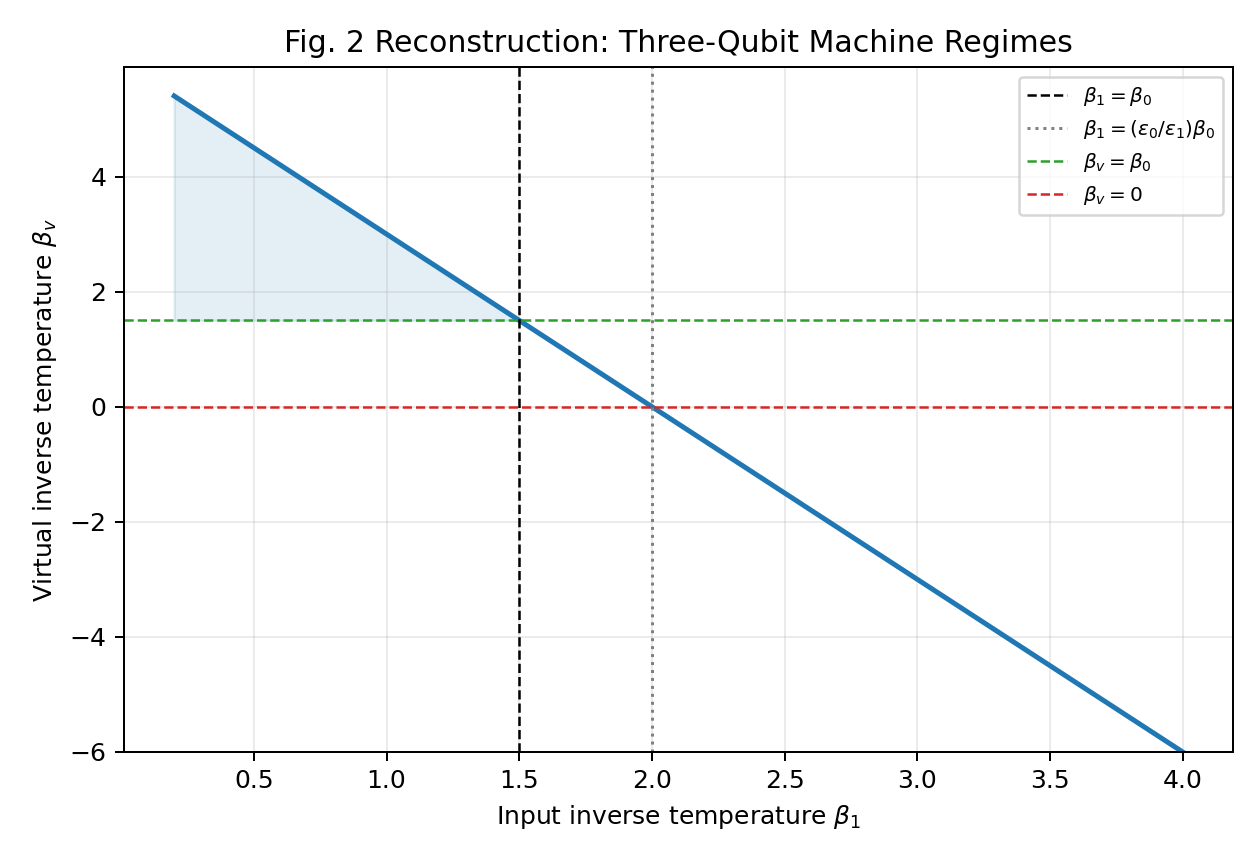
\includegraphics[width=0.72\linewidth]{fig2_virtual_temperature_regimes.png}
\caption{Reconstructed virtual--temperature regimes of the collector,
validating the sign and scale of \eqref{eq:betav} before any decoding.}
\label{fig:virt-regimes}
\end{figure}

\begin{figure}[H]\centering
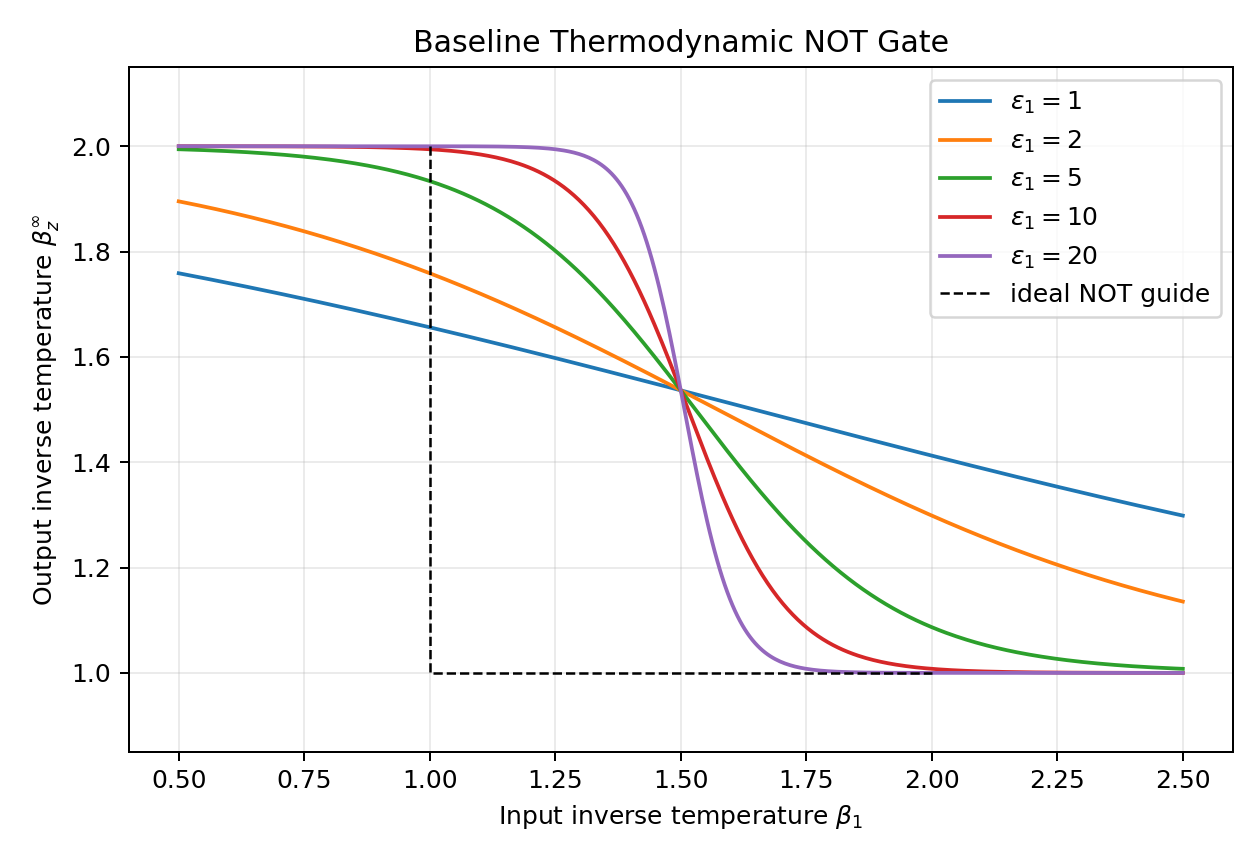
\includegraphics[width=0.72\linewidth]{not_gate_transfer_curves.png}
\caption{Reconstructed NOT transfer curves \eqref{eq:transfer} for several
collector energy scales. The gate is realized when the hot-- and
cold--input outputs lie on opposite sides of $\beta_{\mathrm{th}}$;
increasing $\epsilon_1$ sharpens the curve toward the ideal step.}
\label{fig:not-curves}
\end{figure}

\begin{figure}[H]\centering

\includegraphics[width=0.68\linewidth]{fig3c_error_dissipation_tradeoff.png}
\caption{Reconstructed error--dissipation trade--off: lowering the
decoding error requires larger entropy production, as anticipated in
Section~\ref{sec:logic}.}
\label{fig:err-diss}
\end{figure}

\begin{table}[H]\centering\small
\caption{Representative error--dissipation data for increasing collector
energy scale $\epsilon_1$ (uniform inputs).}
\label{tab:err-diss}
\begin{tabular}{rrrr}
\toprule
$\epsilon_1$ & Average error & Average entropy production & Hot-input output \\
\midrule
1  & $1.6477\times10^{-1}$ & $3.7266\times10^{4}$ & 1.6561 \\
2  & $3.1114\times10^{-2}$ & $2.8675\times10^{5}$ & 1.7588 \\
5  & $2.1882\times10^{-4}$ & $3.1029\times10^{6}$ & 1.9338 \\
10 & $1.9770\times10^{-5}$ & $9.5496\times10^{6}$ & 1.9942 \\
20 & $1.5480\times10^{-5}$ & $1.9882\times10^{7}$ & 2.0000 \\
\bottomrule
\end{tabular}
\end{table}

The same reconstruction reproduces multi--input and composed logic:
the NOR response surface (Fig.~\ref{fig:nor}), the three--input majority
response (Fig.~\ref{fig:maj}), and an XOR network assembled from
thermodynamic--neuron subgates (Fig.~\ref{fig:xor}), consistent with the
perceptron correspondence of Section~\ref{sec:general}.

\begin{figure}[H]\centering
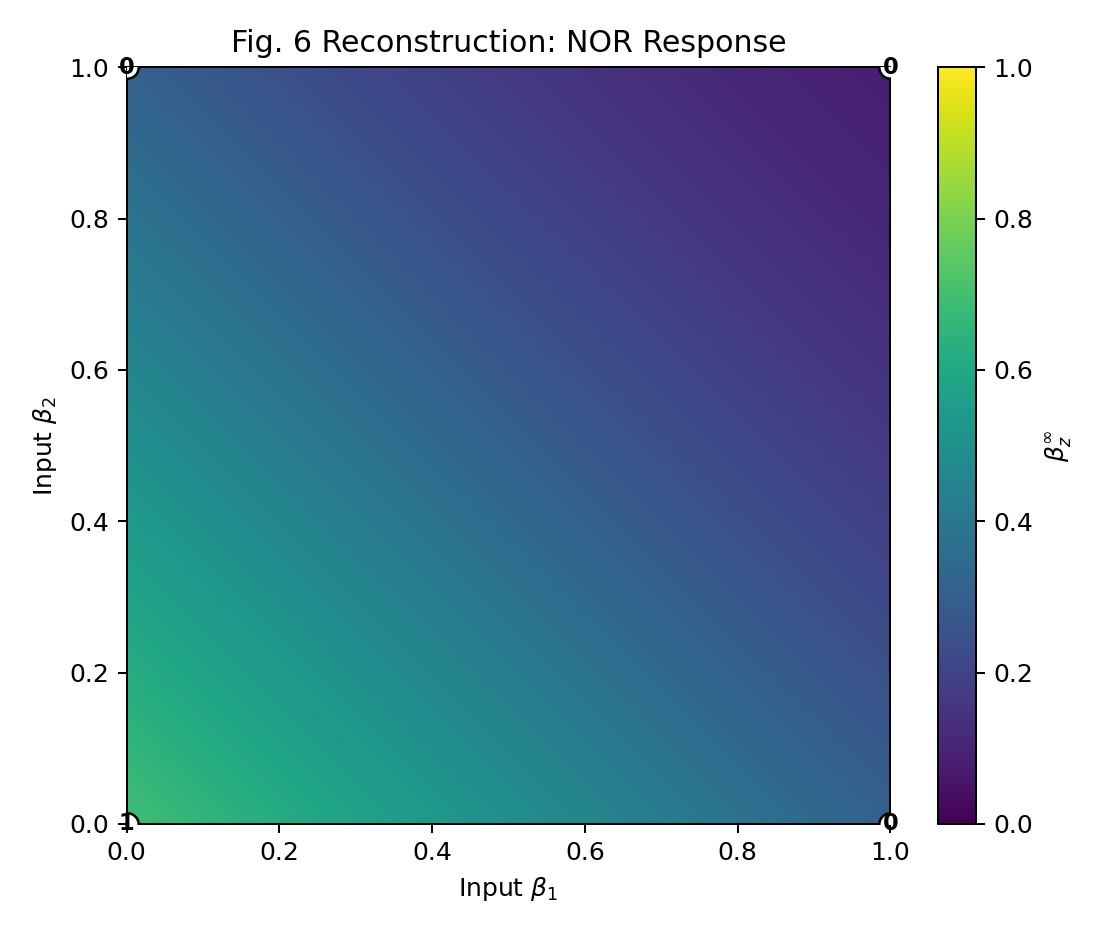
\includegraphics[width=0.70\linewidth]{fig6_nor_response_surface.png}
\caption{Reconstructed NOR response surface: high output only near the
low--low input corner.}
\label{fig:nor}
\end{figure}
\begin{figure}[H]\centering
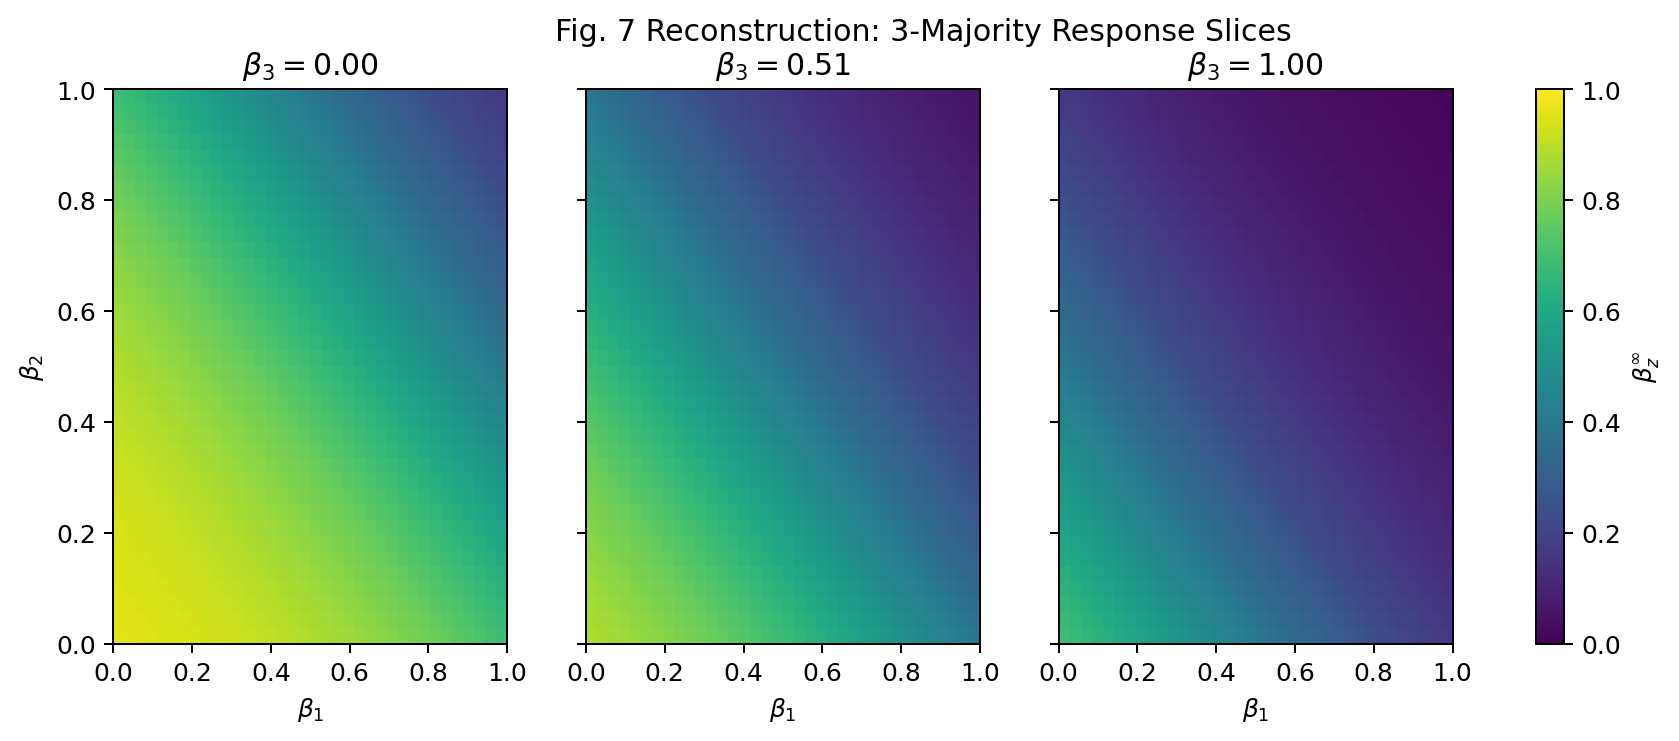
\includegraphics[width=0.70\linewidth]{fig7_majority_response_slices.png}
\caption{Reconstructed three--input majority response (two--dimensional
slices), a linear thermodynamic score of the input temperatures.}
\label{fig:maj}
\end{figure}
\begin{figure}[H]\centering
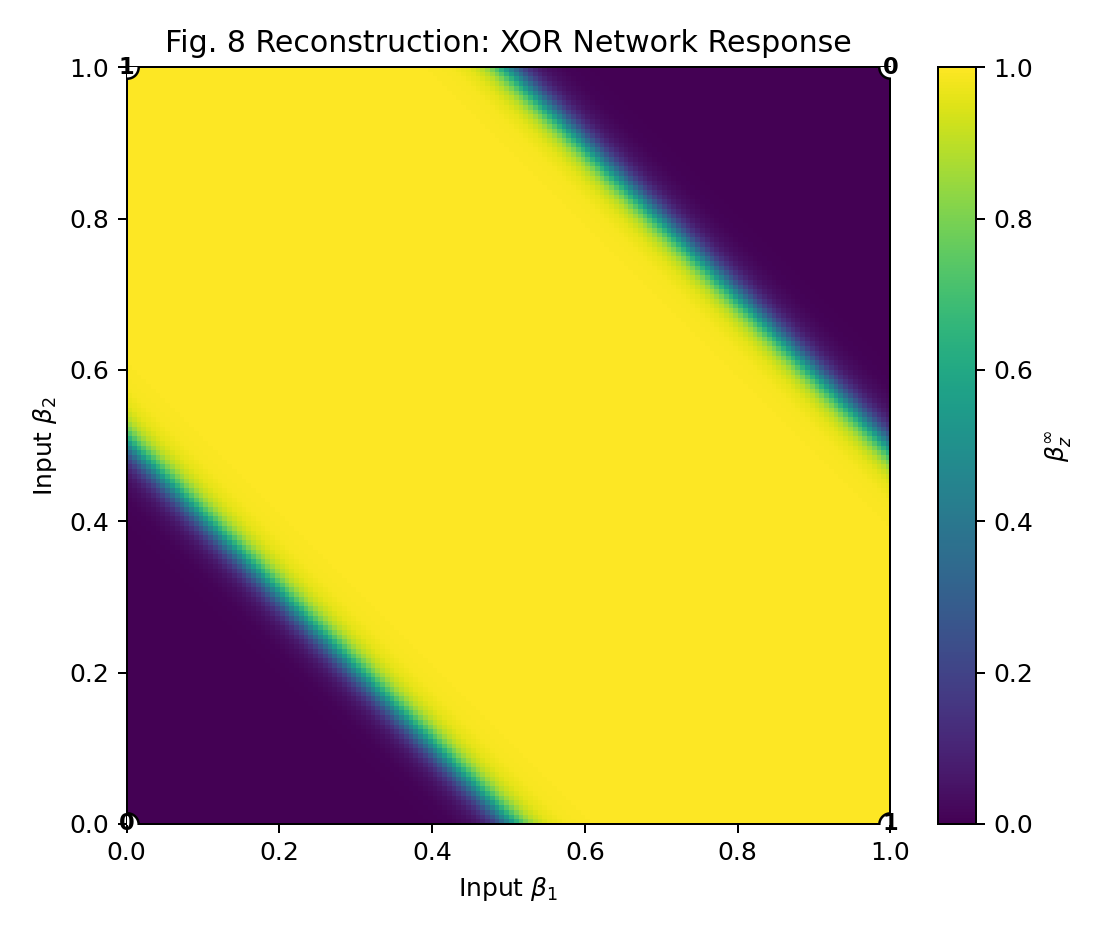
\includegraphics[width=0.70\linewidth]{fig8_xor_network_response.png}
\caption{Reconstructed XOR response from a small network of neurons;
XOR is not linearly separable and cannot be a single perceptron.}
\label{fig:xor}
\end{figure}

\section{Beyond weak coupling: non--Markovian dynamics}
\label{sec:nonmarkov}
The reset model rests on the whole approximation chain of
Table~\ref{tab:approximations}. For a \emph{structured} reservoir the
Markov step (A3) is the first to fail: the memory kernel $\calK$ of the
exact Nakajima--Zwanzig equation \eqref{eq:NZ} is no longer sharply
peaked, and the reduced motion
\begin{equation}
\dot\rho_S(t)=-\ii[H_S,\rho_S(t)]
+\int_0^t\calK(t-\tau)\rho_S(\tau)\,\d\tau
\end{equation}
retains genuine history dependence: revivals, information backflow, and
modified relaxation. A strong claim about non--Markovian thermodynamic
logic therefore requires a numerically exact treatment of the memory,
not a Lindblad surrogate.

\subsection{Influence functional and process tensor}
For a Gaussian bosonic bath linearly coupled to the system, the bath can
be integrated out exactly. On a forward--backward path pair
$(s^+,s^-)$ the reduced propagator carries the Feynman--Vernon influence
functional
\begin{equation}
\mathcal F[s^+,s^-]
=\exp\!\Big[-\!\int_0^t\!\d\tau\!\int_0^\tau\!\d\tau'\,
(s^+_\tau-s^-_\tau)\big(\eta(\tau-\tau')s^+_{\tau'}
-\eta^\ast(\tau-\tau')s^-_{\tau'}\big)\Big],
\end{equation}
with the bath response kernel set by the spectral density,
\begin{equation}
\eta(t)=\int_0^\infty\!\d\omega\,J(\omega)
\Big[\coth\!\big(\tfrac{\beta\omega}{2}\big)\cos\omega t-\ii\sin\omega t\Big],
\qquad J(\omega)=2\alpha\,\omega^s\ee^{-\omega/\omega_c}.
\label{eq:influence}
\end{equation}
Discretizing time into $N$ slices makes the influence functional a
multilinear object --- the \emph{process tensor} --- mapping a sequence of
control operations $\mathcal A_0,\ldots,\mathcal A_{N-1}$ to the final
state,
\begin{equation}
\rho_N=\Upsilon_{N:0}\star(\mathcal A_{N-1}\otimes\cdots\otimes\mathcal A_0),
\qquad
\Upsilon_{N:0}=\sum_{\{\alpha_k\}}M^{[N]}_{\alpha_{N-1}}\cdots
M^{[1]}_{\alpha_0}M^{[0]} .
\label{eq:PT}
\end{equation}

\subsection{MPS, MPO, TTN and why memory is compressible}
Written as a matrix product operator along the time axis, the process
tensor has bond dimension $\chi$ measuring the memory carried from past to
future:
\begin{equation}
\Upsilon=\sum_{\{i_k,j_k\}}W^{[0]i_0j_0}\cdots W^{[N]i_Nj_N}
\ket{i_0\cdots i_N}\bra{j_0\cdots j_N} .
\end{equation}
A Markovian bath has $\chi=1$; a non--Markovian but compressible bath has
$1<\chi\ll d^{2N}$, so singular--value truncation keeps the physically
relevant temporal correlations without the exponential blow--up of an
explicit system--plus--bath simulation (dimension $d_Sd^N$). A
tree--tensor--network (TTN) generalization places each reservoir of the
neuron on a separate branch, which is why the numerical programme lists
PT--MPO/TEMPO as the primary structured--bath backend and TTN as the
fallback when memory growth dominates. This is the same chain / MPS
machinery treated rigorously in Part~\ref{part:abhishek}.

\subsection{A single worked example: from the memory kernel to output logic}
Consider one logical qubit coupled to a structured bath through a driven
buffer, $S\leftrightarrow F(t)\leftrightarrow B$. (1) The full state obeys
$\dot\rho_{SFB}=-\ii[H_{SFB}(t),\rho_{SFB}]$ and the logical state is
$\rho_S=\Tr_{FB}\rho_{SFB}$. (2) Tracing out buffer and bath gives a
driven memory kernel $\calK_F(t,\tau)$; tuning the drive $(A,\Omega)$
reshapes $\calK_F$ and hence how information leaves or returns to the
qubit. (3) Rather than construct $\calK_F$ explicitly, the process--tensor
method builds $\Upsilon_{n:0}$ and contracts it with the system operations
\eqref{eq:PT}. (4) For a binary gate, evolve two inputs
$\rho_S^{(0)}(0),\rho_S^{(1)}(0)$ and read the distinguishability
\begin{equation}
D_{\mathrm{out}}=\tfrac12\big\|\rho_S^{(0)}(t_f)-\rho_S^{(1)}(t_f)\big\|_1 .
\label{eq:tracedist}
\end{equation}
The buffer is useful only if it improves $D_{\mathrm{out}}$ (or the
decoding margin) at an acceptable drive cost.

\subsection{Structured--bath benchmark and convergence}
Before any gate claim, the solver must pass numerical--health checks:
trace preservation $\delta_{\mathrm{tr}}=|\Tr\rho-1|$, Hermiticity
$\delta_{\mathrm{herm}}=\|\rho-\rho^\dagger\|_F$, and convergence under
$\Delta t$ and memory time $\tau_{\mathrm{mem}}$. A single qubit in the
bath \eqref{eq:influence} was tracked across sub--Ohmic, Ohmic, and
super--Ohmic regimes (Table~\ref{tab:struct-bath},
Fig.~\ref{fig:nonmarkov}); the largest trace deviation was
$1.884\times10^{-5}$ and the largest Hermiticity error
$5.011\times10^{-7}$, with working point
$(\Delta t,\tau_{\mathrm{mem}},\chi_{\mathrm{svd}})=(0.05,1.0,10^{-6})$.
A first quick scan failed the $10^{-3}$ criterion ($4.234\times10^{-3}$);
refining $\Delta t$ at fixed $\tau_{\mathrm{mem}}=1.0$ reduced the drift
to $6.579\times10^{-4}$ (pass).

\begin{table}[H]\centering\small
\caption{Single--qubit structured--bath benchmark across spectral regimes.}
\label{tab:struct-bath}
\begin{tabular}{lrrrr}
\toprule
Regime & $s$ & Final purity & Final $\sigma_z$ & Runtime (s) \\
\midrule
Sub-Ohmic & 0.5 & 0.5070 & $-0.1184$ & 20.996 \\
Ohmic & 1.0 & 0.5248 & $0.2230$ & 6.582 \\
Super-Ohmic & 3.0 & 0.8421 & $0.8272$ & 4.479 \\
\bottomrule
\end{tabular}
\end{table}

\begin{figure}[H]\centering
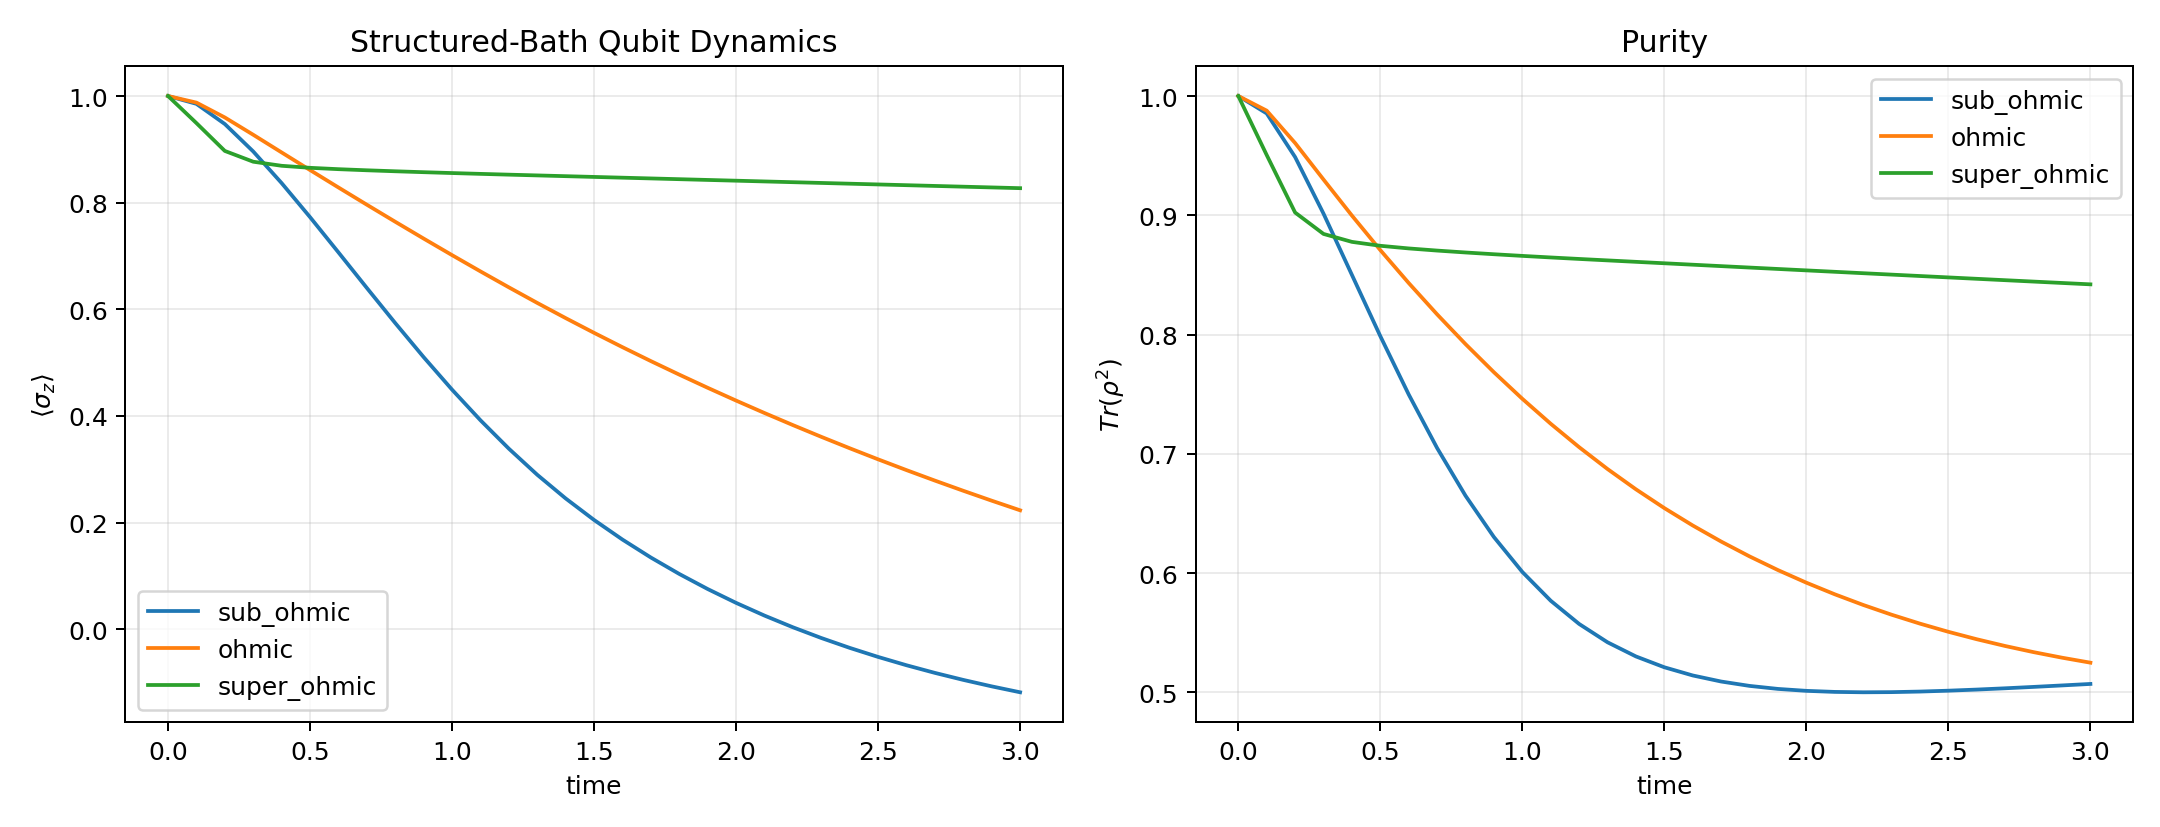
\includegraphics[width=0.72\linewidth]{single_qubit_research_regime_comparison.png}
\caption{Reduced single--qubit dynamics for three structured--bath
regimes --- the numerical bridge between the Markovian neuron and later
memory--bearing gate simulations.}
\label{fig:nonmarkov}
\end{figure}
\begin{figure}[H]\centering
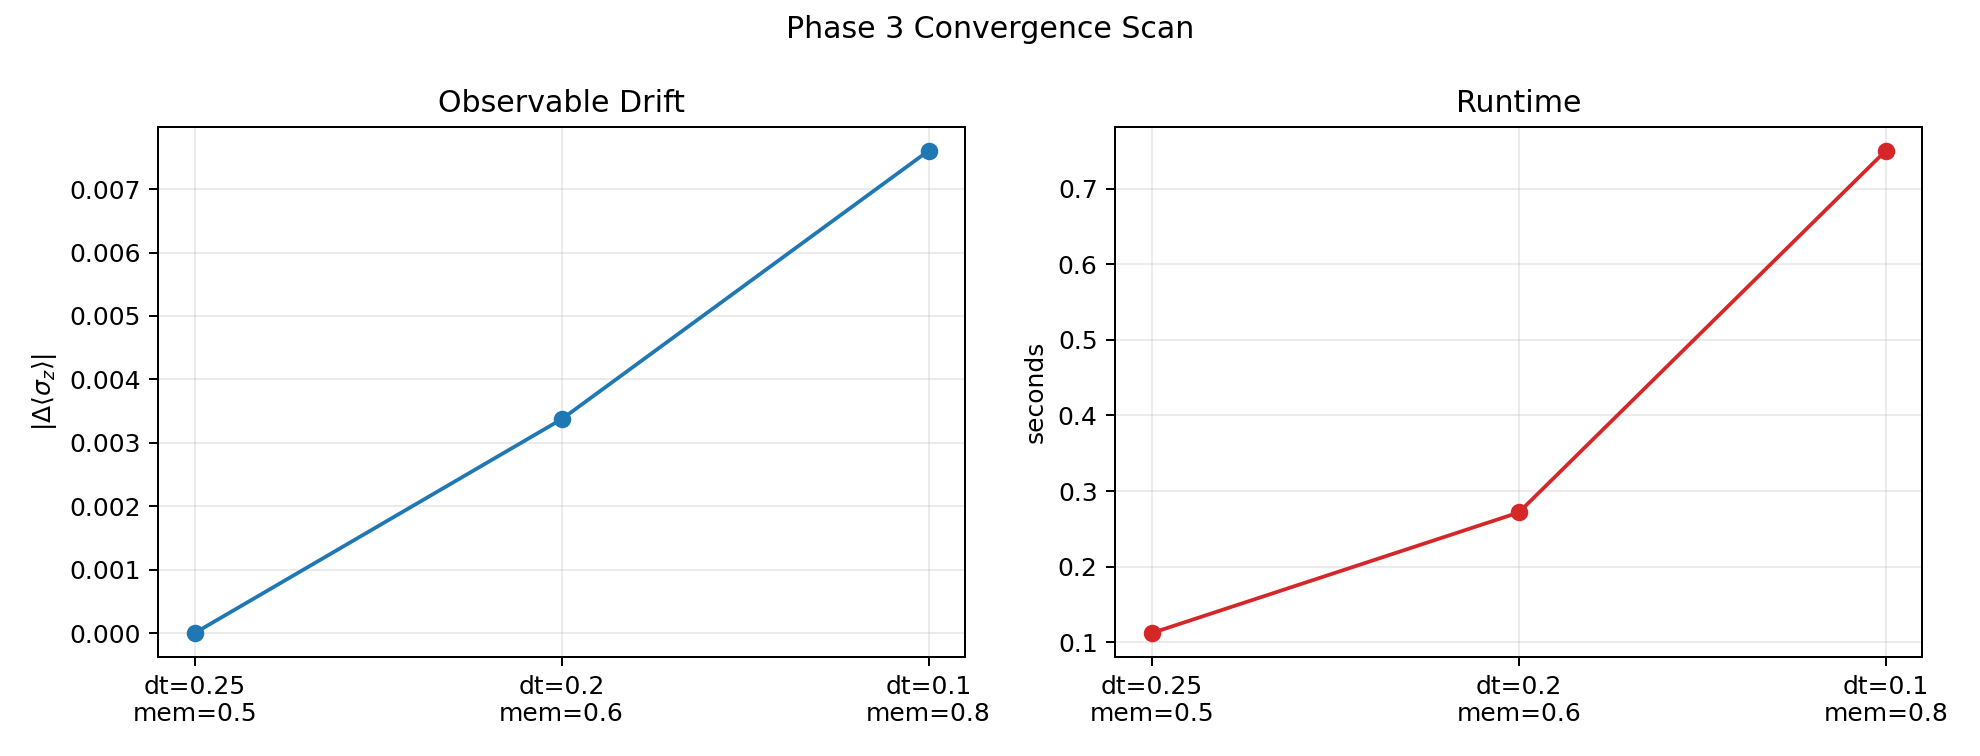
\includegraphics[width=0.70\linewidth]{convergence_scan_quick.png}
\caption{Quick convergence scan (structured--bath benchmark), used as a
deliberate failure mode before interpreting non--Markovian logic.}
\label{fig:conv}
\end{figure}

\section{The Floquet buffer}
\label{sec:floquet}
To reduce the logical qubit's direct exposure to the reservoir, a
periodically driven buffer is inserted between subsystem and bath,
\begin{equation}
S\longleftrightarrow F(t)\longleftrightarrow B
\qquad\text{versus the direct}\qquad
S\longleftrightarrow B .
\end{equation}
A minimal buffer Hamiltonian, as implemented in the bridge code, is
\begin{equation}
H_F(t)=\tfrac{\epsilon_F}{2}\sigma_z+A\cos(\Omega t)\sigma_x,\qquad
H_{SF}=g_{SF}\,\sigma_x^{(S)}\!\otimes\sigma_x^{(F)},\qquad
T=\tfrac{2\pi}{\Omega},
\label{eq:bufferH}
\end{equation}
so the full bridge Hamiltonian is $H(t)=H_S+H_F(t)+H_{SF}+H_B+H_{FB}$.
(The refined, purely longitudinal drive that yields clean Bessel
sidebands is analyzed rigorously in Part~\ref{part:abhishek}; here we keep
the minimal implemented form.) In a weak Markovian treatment of the
buffer--bath contact the logical qubit sees a time--periodic generator
$\dot\rho_S=\calL_{\mathrm{eff}}(t)\rho_S$,
$\calL_{\mathrm{eff}}(t+T)=\calL_{\mathrm{eff}}(t)$, whose rates sample the
bath at drive--shifted frequencies $\omega+n\Omega$. This is the origin of
Floquet filtering: the buffer presents the effective spectral density
\begin{equation}
J_{\mathrm{eff}}(\omega)=\sum_n|c_n(A,\Omega)|^2\,J(\omega+n\Omega),
\label{eq:Jeff}
\end{equation}
whose weights $|c_n|^2$ are set by the drive.

\begin{figure}[H]
\centering
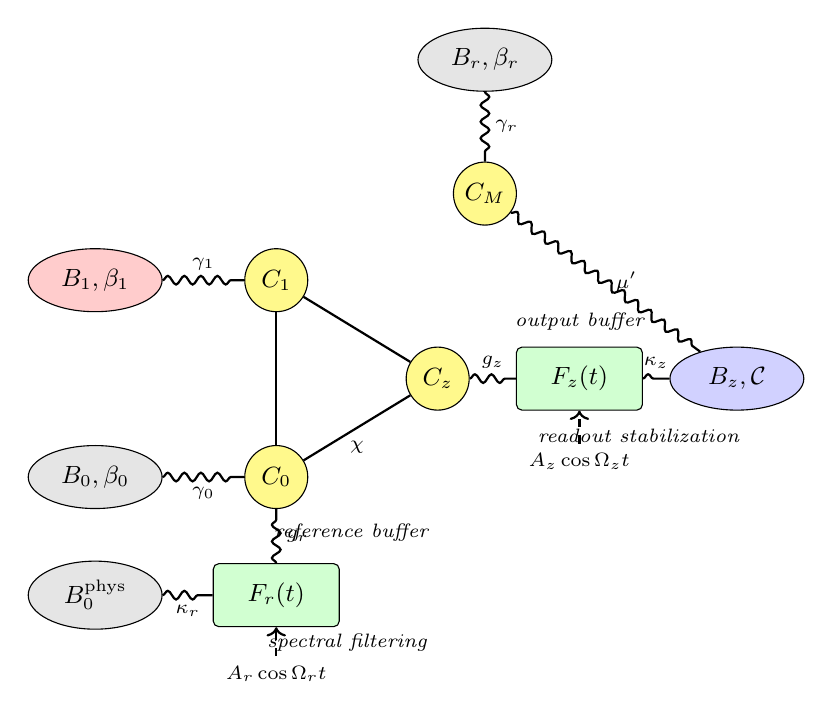
\begin{tikzpicture}[
  qubit/.style={circle, draw, fill=yellow!45, minimum size=8mm,
                inner sep=1pt, font=\small},
  bath/.style={ellipse, draw, fill=gray!20, minimum width=17mm,
               minimum height=8mm, font=\small},
  hotbath/.style={ellipse, draw, fill=red!20, minimum width=17mm,
                  minimum height=8mm, font=\small},
  outbath/.style={ellipse, draw, fill=blue!18, minimum width=17mm,
                  minimum height=8mm, font=\small},
  buffer/.style={rectangle, draw, fill=green!18, rounded corners=2pt,
                 minimum width=16mm, minimum height=8mm, font=\small},
  therm/.style={decorate, decoration={snake, amplitude=.55mm,
                segment length=2.1mm, post length=1.0mm}, thick},
  coh/.style={thick},
  drive/.style={->, dashed, thick}
]
\node[hotbath] (B1) at (0,1.25) {$B_1,\beta_1$};
\node[bath]    (B0) at (0,-1.25) {$B_0,\beta_0$};
\node[qubit]   (C1) at (2.3,1.25) {$C_1$};
\node[qubit]   (C0) at (2.3,-1.25) {$C_0$};
\node[qubit]   (Cz) at (4.35,0) {$C_z$};
\node[qubit]   (CM) at (4.95,2.35) {$C_M$};
\node[bath]    (Br) at (4.95,4.05) {$B_r,\beta_r$};
\node[buffer]  (Fr) at (2.3,-2.75) {$F_r(t)$};
\node[bath]    (B0phys) at (0,-2.75) {$B_0^{\rm phys}$};
\node[buffer]  (Fz) at (6.15,0) {$F_z(t)$};
\node[outbath] (Bz) at (8.15,0) {$B_z,\mathcal C$};
\node[font=\scriptsize] (dr1) at (2.3,-3.75) {$A_r\cos\Omega_r t$};
\node[font=\scriptsize] (dr2) at (6.15,-1.05) {$A_z\cos\Omega_z t$};

\draw[therm] (B1) -- (C1) node[midway,above,font=\scriptsize]{$\gamma_1$};
\draw[therm] (B0) -- (C0) node[midway,below,font=\scriptsize]{$\gamma_0$};
\draw[coh] (C0) -- (C1);
\draw[coh] (C1) -- (Cz);
\draw[coh] (C0) -- (Cz) node[midway,below=1pt,font=\scriptsize]{$\chi$};
\draw[therm] (Br) -- (CM) node[midway,right,font=\scriptsize]{$\gamma_r$};
\draw[therm] (CM) -- (Bz) node[midway,right,font=\scriptsize]{$\mu'$};
\draw[therm] (B0phys) -- (Fr) node[midway,below,font=\scriptsize]{$\kappa_r$};
\draw[therm] (Fr) -- (C0) node[midway,right,font=\scriptsize]{$g_r$};
\draw[therm] (Cz) -- (Fz) node[midway,above,font=\scriptsize]{$g_z$};
\draw[therm] (Fz) -- (Bz) node[midway,above,font=\scriptsize]{$\kappa_z$};
\draw[drive] (dr1) -- (Fr);
\draw[drive] (dr2) -- (Fz);

\node[font=\scriptsize\itshape] at (3.25,-1.95) {reference buffer};
\node[font=\scriptsize\itshape] at (6.15,0.72) {output buffer};
\node[font=\scriptsize\itshape] at (3.2,-3.35) {spectral filtering};
\node[font=\scriptsize\itshape] at (6.9,-0.72) {readout stabilization};
\end{tikzpicture}
\caption{Floquet--buffered thermodynamic neuron architecture.  The
collector still forms the virtual temperature through the coherent
three--body interaction among $C_0,C_1,C_z$, while driven intermediate
systems $F_r(t)$ and $F_z(t)$ regulate the reference and output reservoir
contacts.  The direct autonomous contact is recovered by setting the
buffer couplings to zero and reconnecting the corresponding bath
directly to the qubit.}
\label{fig:floquet-full-architecture}
\end{figure}

\subsection{Operational metrics}
The buffer is assessed operationally by the output trace distance
\eqref{eq:tracedist} and by the drive--work proxy
\begin{equation}
W_{\mathrm{proxy}}=\int_0^{t_f}\Tr\!\big[\rho(t)\,\dot H_F(t)\big]\d t
=-A\Omega\int_0^{t_f}\sin(\Omega t)\,\langle\sigma_x\rangle_t\,\d t .
\label{eq:wproxy}
\end{equation}
This is an operational indicator, not a full strong--coupling
thermodynamic audit (which must also track interaction and bath energy,
cf.\ approximation (A11)).

\subsection{Screening and ablation}
A single run is insufficient evidence. Screening over drive amplitude,
drive frequency and system--buffer coupling found positive trace--distance
gain $\Delta D=D_{\mathrm{buffer}}-D_{\mathrm{direct}}$ in $14$ of $15$
configurations, with best gain $0.711315$ at weak system--buffer coupling.
The ablation (Table~\ref{tab:ablation}) isolates the drive: with $A=0$ the
buffer is a passive spacer and \emph{degrades} distinguishability
($\Delta D=-0.149461$); the benefit appears only under periodic
modulation, consistent with the sideband picture \eqref{eq:Jeff}. The
strongest gain at weak $g_{SF}$ indicates the buffer acts as a selective
mediated channel rather than a strongly hybridized extra degree of
freedom.

\begin{table}[H]\centering\small
\caption{Ablation of the Floquet--buffer bridge. Direct baseline
$D_{\mathrm{direct}}(t_f)=0.236928$; gain
$\Delta D=D_{\mathrm{buffer}}-D_{\mathrm{direct}}$.}
\label{tab:ablation}
\begin{tabular}{lrrrr}
\toprule
Case & $D_{\mathrm{buffer}}(t_f)$ & $\Delta D$ & Relative gain & $|W_{\mathrm{proxy}}|$ \\
\midrule
Full driven buffer & 0.320480 & 0.083551 & 0.352644 & 0.176530 \\
No periodic drive & 0.087467 & $-0.149461$ & $-0.630829$ & 0 \\
Weak drive & 0.372211 & 0.135282 & 0.570984 & 0.086262 \\
Strong drive & 0.401688 & 0.164760 & 0.695401 & 0.087613 \\
Weak system--buffer coupling & 0.948243 & 0.711315 & 3.002237 & 0.019354 \\
Strong system--buffer coupling & 0.601144 & 0.364215 & 1.537240 & 0.439431 \\
Weak buffer--bath contact & 0.237160 & 0.000232 & 0.000979 & 0.021202 \\
Strong buffer--bath contact & 0.405590 & 0.168662 & 0.711869 & 0.398363 \\
\bottomrule
\end{tabular}
\end{table}

\begin{figure}[H]\centering
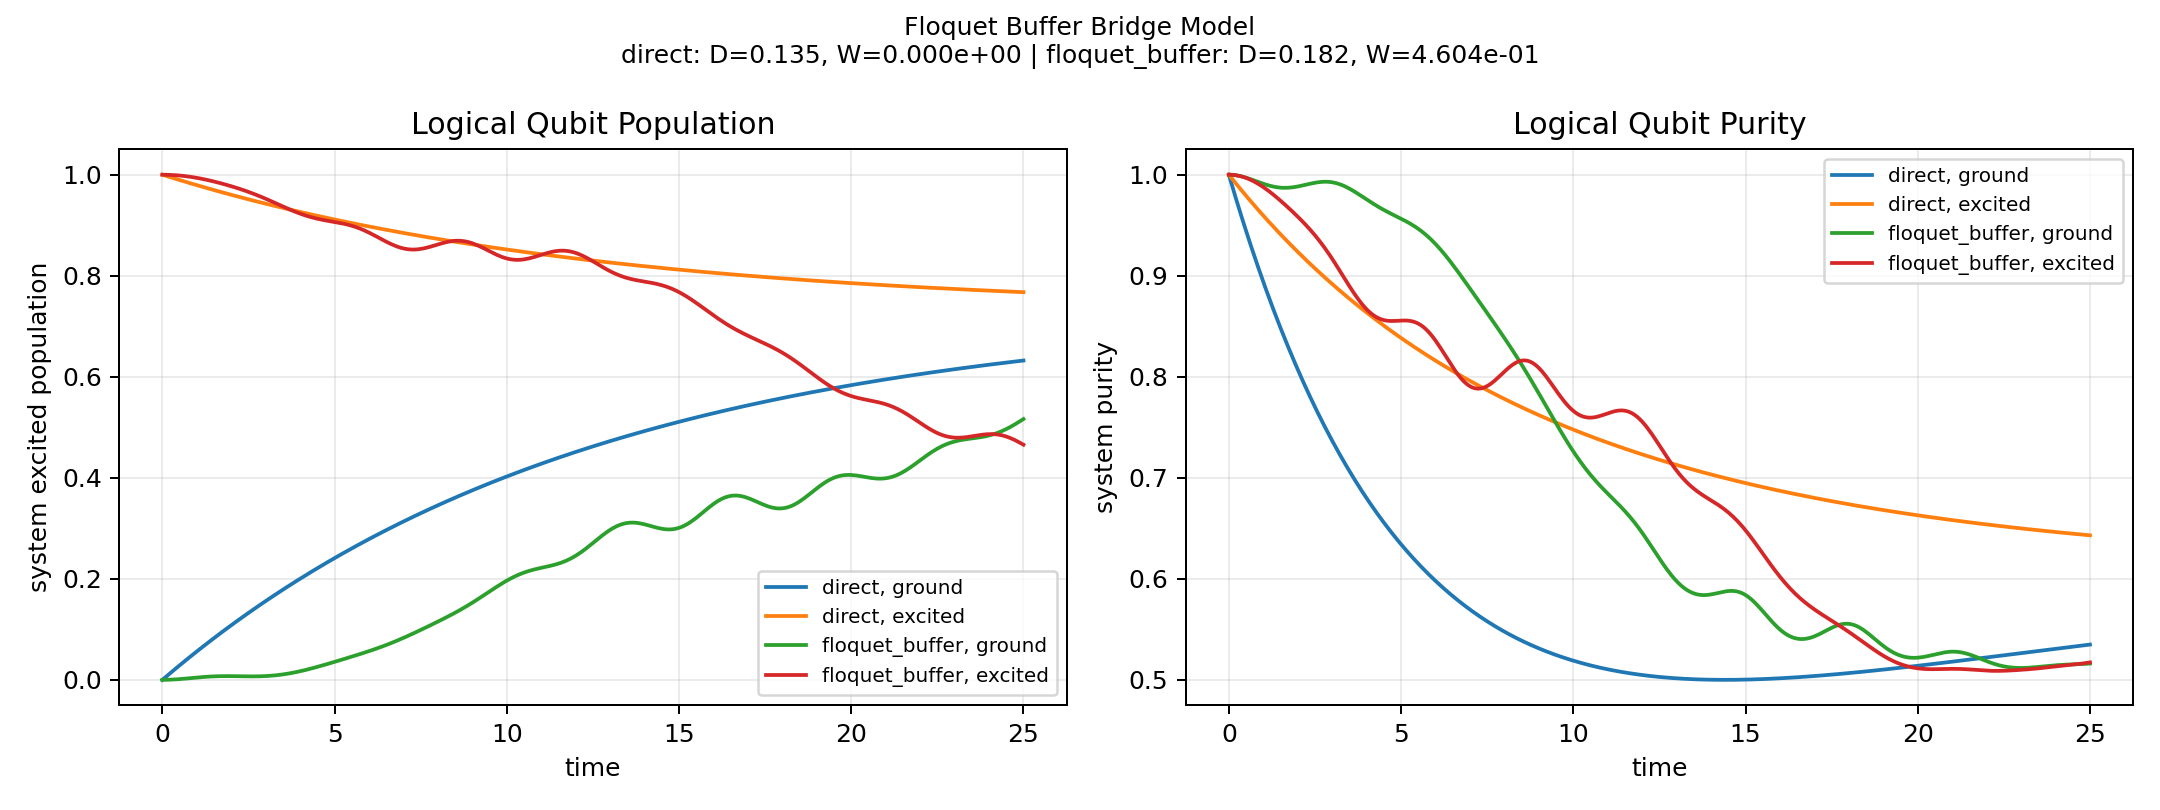
\includegraphics[width=0.70\linewidth]{floquet_buffer_comparison.png}
\caption{Direct versus Floquet--buffered dynamics in the bridge model.}
\label{fig:floq-comp}
\end{figure}
\begin{figure}[H]\centering
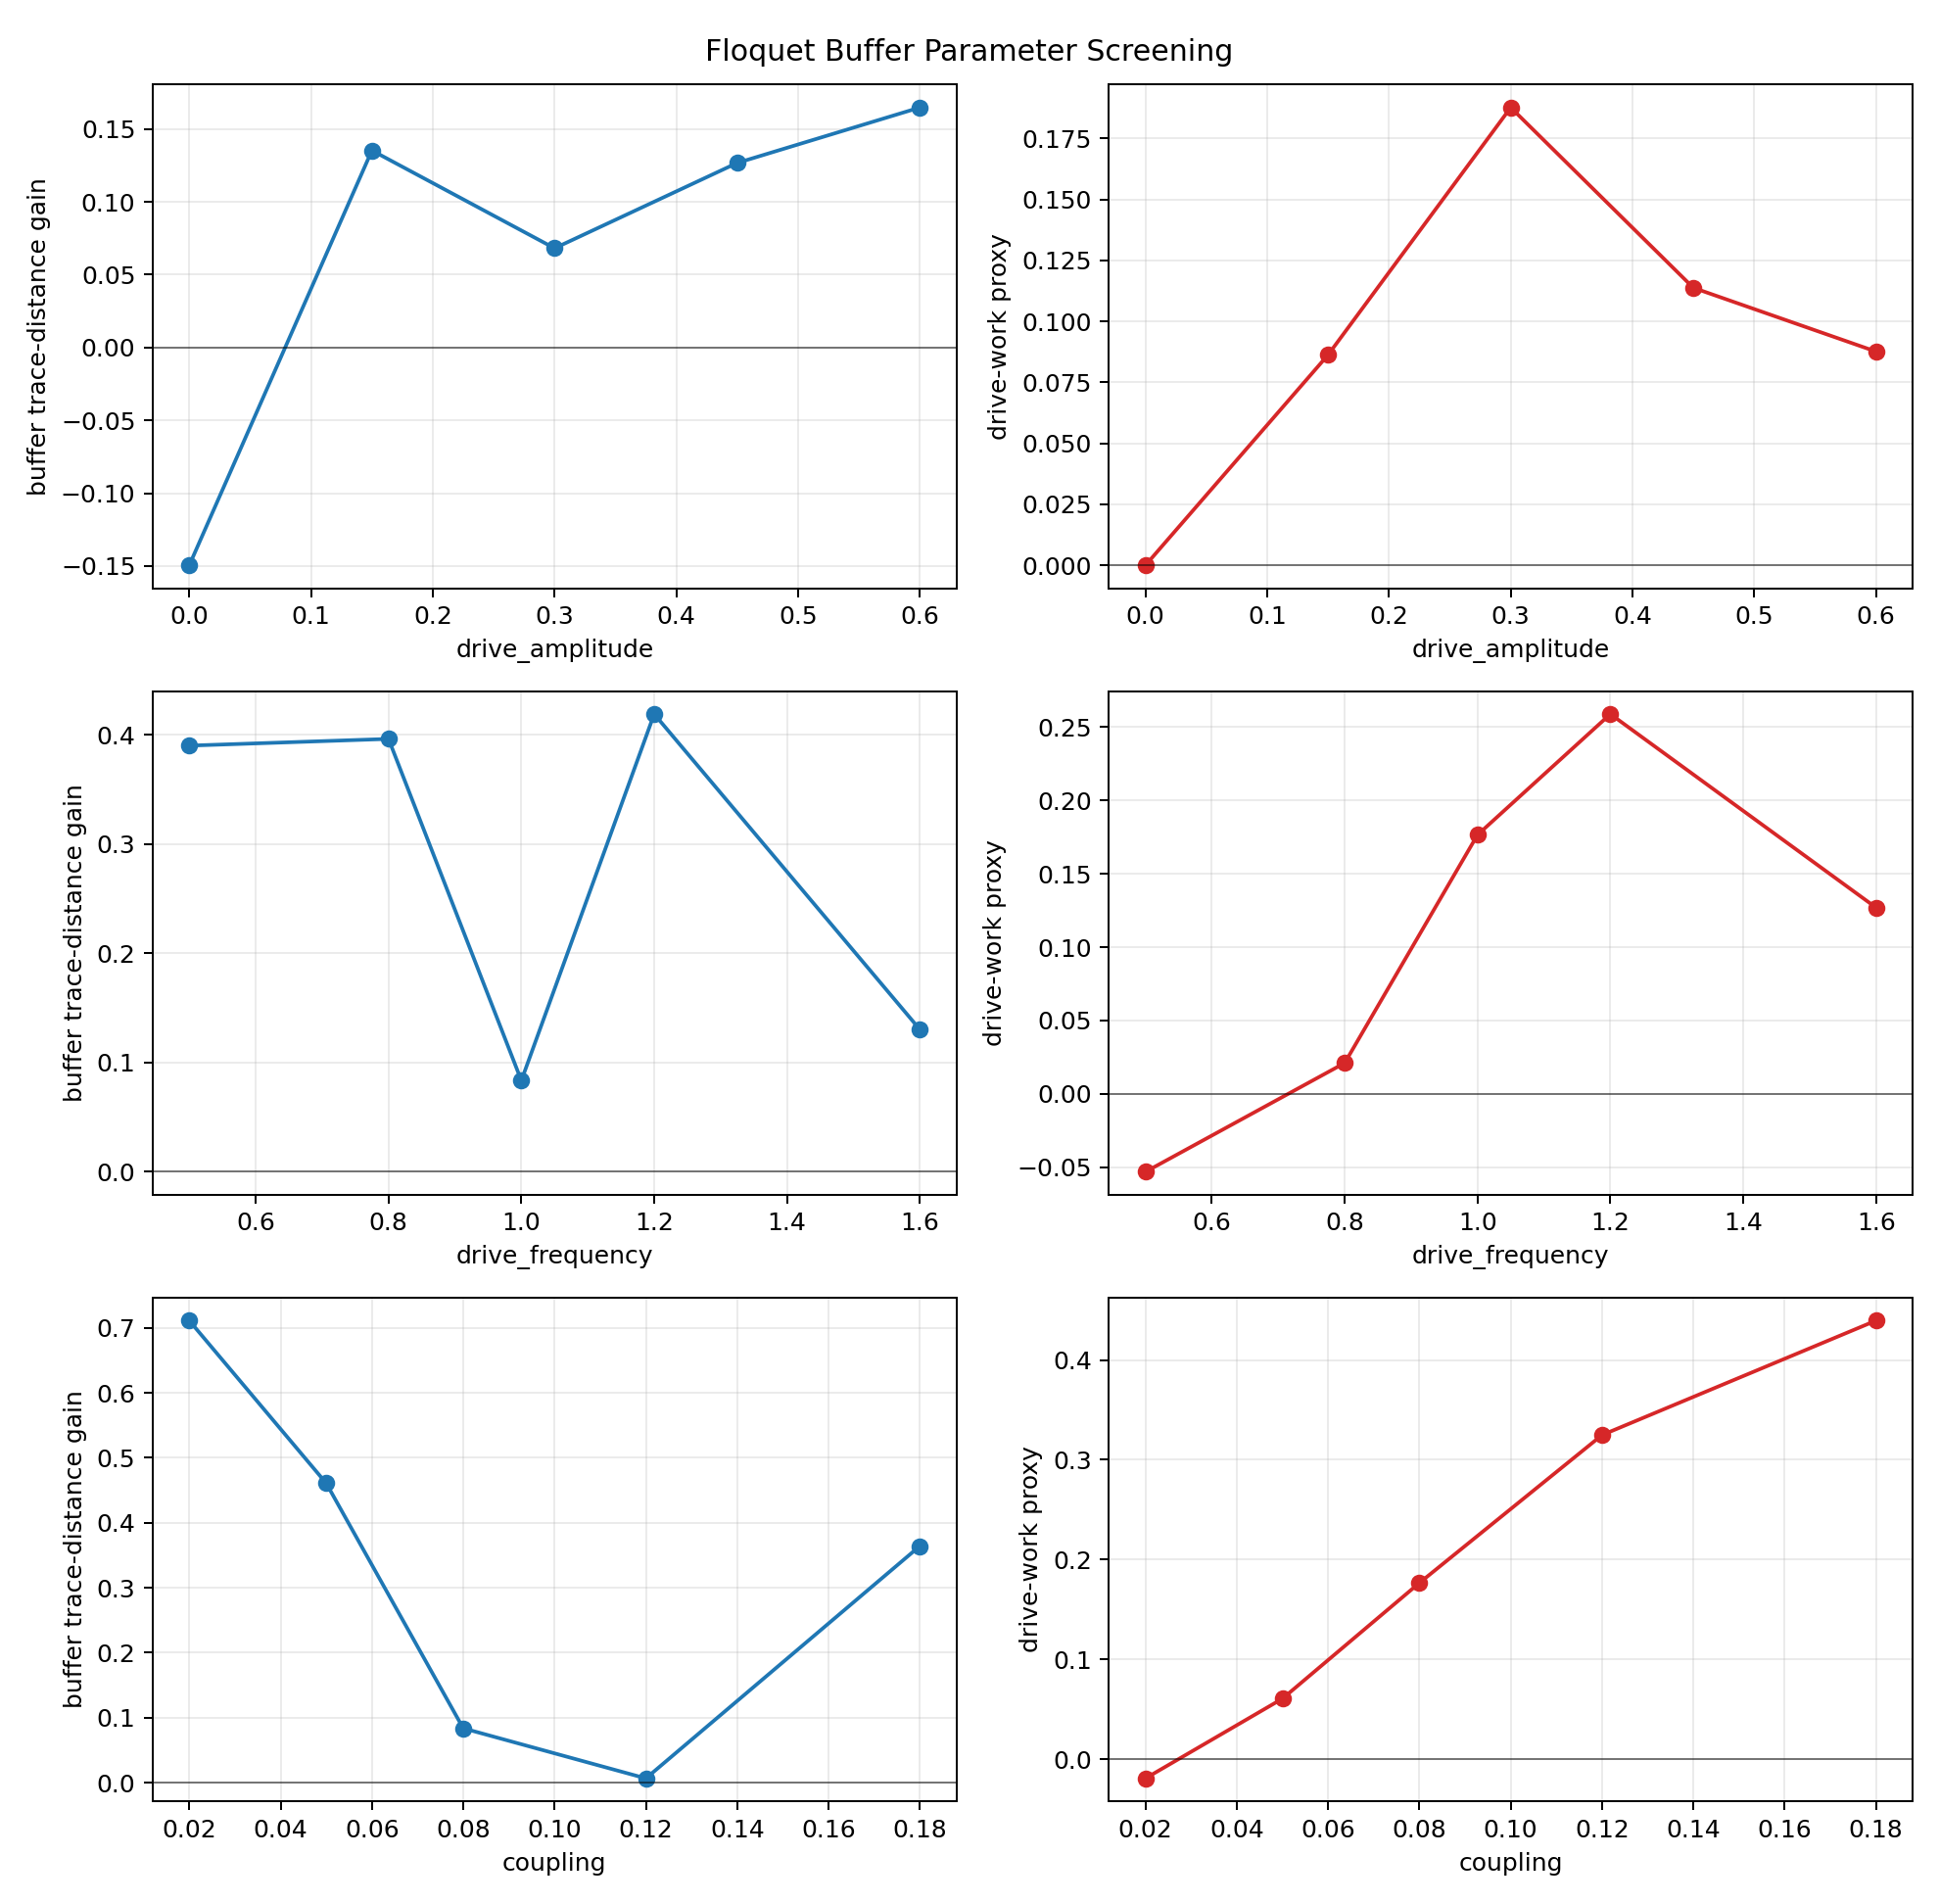
\includegraphics[width=0.70\linewidth]{floquet_parameter_sweep.png}
\caption{Floquet parameter sweep; best screened trace--distance gain
$0.711315$.}
\label{fig:floq-sweep}
\end{figure}

Embedding the buffer in the full three--qubit NOT surrogate preserves the
truth table: both direct and buffered GKSL surrogates give
$\calA_{\mathrm{NOT}}=1$ with small drive--work proxy
(Table~\ref{tab:outcomes}). Under the Phase~V PT--MPO/TEMPO structured
bath the calibrated decoder (architecture--specific threshold
$\beta_{\mathrm{th}}^{(a)}=\tfrac12[\beta_{\mathrm{eff}}^{(a)}(0)
+\beta_{\mathrm{eff}}^{(a)}(1)]$) also passes, but the buffered margin is
small ($\sim2.6\times10^{-5}$ versus a direct margin $\sim1.43\times10^{-1}$)
--- truth--table passing is binary, robustness is a margin statement.

\begin{table}[H]\centering\small
\caption{Main numerical outcomes across the staged programme.
$\calA_{\mathrm{NOT}}$ is truth--table accuracy; $D(t_f)$ the final
logical trace distance.}
\label{tab:outcomes}
\begin{tabular}{@{}p{0.30\linewidth}p{0.20\linewidth}p{0.18\linewidth}p{0.24\linewidth}@{}}
\toprule
Experiment & Metric & Result & Interpretation \\
\midrule
Floquet bridge & $\Delta D$ & $0.0836$ / $0.711$ best & driven buffer can improve distinguishability \\
No--drive ablation & $\Delta D$ & $-0.1495$ & passive buffer degrades; drive essential \\
3--qubit GKSL direct & $\calA_{\mathrm{NOT}},D$ & $1.000,\,0.0249$ & direct NOT passes \\
3--qubit GKSL buffered & $\calA_{\mathrm{NOT}},D$ & $1.000,\,0.0241$ & buffered NOT passes \\
PT--MPO/TEMPO direct & $\calA_{\mathrm{NOT}}$, margin & $1.000,\,1.43\times10^{-1}$ & structured--bath direct passes \\
PT--MPO/TEMPO buffered & $\calA_{\mathrm{NOT}}$, margin & $1.000,\,2.60\times10^{-5}$ & passes, close to boundary \\
GKSL phase map & robust points & $68/80$ & broad passing region \\
\bottomrule
\end{tabular}
\end{table}

\section{Full GKSL, HEOM, and tensor--network gate validation}
\label{sec:heom-mps-validation}
The final physics claim cannot rest on the bridge model alone. The
complete validation stack should solve the same gate at three levels of
description and demand that the logical truth table and the buffer
advantage survive refinement.

\subsection{Level 1: full time--dependent GKSL gate}
The Markovian full-gate baseline keeps the collector, modulator, and
buffer degrees of freedom explicitly in the system Hilbert space,
\begin{equation}
\rho_{\mathrm{sys}}(t)
\in\mathcal{B}\!\left(
\calH_{C_0}\otimes\calH_{C_1}\otimes\calH_{C_z}
\otimes\calH_{C_M}\otimes\calH_{F_r}\otimes\calH_{F_z}
\right),
\end{equation}
and evolves
\begin{equation}
\dot\rho_{\mathrm{sys}}(t)
=-\ii[H_{\mathrm{gate}}(t),\rho_{\mathrm{sys}}(t)]
+\sum_{\alpha}\sum_{\omega}\gamma_{\alpha}(\omega)
\left[
L_{\alpha,\omega}\rho_{\mathrm{sys}}L_{\alpha,\omega}^{\dagger}
-\tfrac12\{L_{\alpha,\omega}^{\dagger}L_{\alpha,\omega},\rho_{\mathrm{sys}}\}
\right],
\label{eq:full-gksl-gate}
\end{equation}
with $H_{\mathrm{gate}}(t)$ containing the resonant collector coupling
$\chi$, the modulator branch, and the driven buffer Hamiltonians
$H_{F_r}(t)$ and $H_{F_z}(t)$. The direct and buffered gates are compared
using identical input temperatures and identical decoding:
\begin{equation}
\calA_{\mathrm{NOT}}
=\frac12\sum_{x\in\{0,1\}}
\mathbf{1}\!\left[
\Theta(\beta_z^\infty(x)-\beta_{\mathrm{th}})=1-x
\right],
\qquad
m=\min_x|\beta_z^\infty(x)-\beta_{\mathrm{th}}|.
\end{equation}
The GKSL level is fast enough for sweeps over drive amplitude $A$, drive
frequency $\Omega$, system--buffer coupling $g_{SF}$, and bath-contact
scale $\kappa$. Its job is to find candidate operating regions, not to
prove strong--coupling physics.

\subsection{Level 2: HEOM benchmark for structured reservoirs}
To include reservoir memory without replacing it by a local dissipator,
each structured bath is represented through a correlation-function
decomposition
\begin{equation}
C_{\alpha}(t)
=\int_0^\infty J_{\alpha}(\omega)
\left[\coth\!\left(\frac{\beta_{\alpha}\omega}{2}\right)\cos\omega t
-\ii\sin\omega t\right]\d\omega
\simeq \sum_{k=0}^{K_\alpha} c_{\alpha k}\,\ee^{-\nu_{\alpha k}t}.
\label{eq:heom-correlation}
\end{equation}
For a Drude--Lorentz bath,
$J_{\alpha}(\omega)=2\lambda_{\alpha}\gamma_{\alpha}
\omega/(\omega^2+\gamma_{\alpha}^2)$, the first exponential has
$\nu_{\alpha0}=\gamma_{\alpha}$ and the remaining terms are Matsubara or
Padé frequencies. The HEOM propagates the physical density matrix
$\rho_{\mathbf{0}}$ together with auxiliary density operators (ADOs)
$\rho_{\mathbf{n}}$:
\begin{align}
\dot\rho_{\mathbf{n}}
&= -\ii[H_{\mathrm{gate}}(t),\rho_{\mathbf{n}}]
-\sum_{\alpha k}n_{\alpha k}\nu_{\alpha k}\rho_{\mathbf{n}}
-\ii\sum_{\alpha}[V_{\alpha},\rho_{\mathbf{n}+\mathbf{e}_{\alpha k}}]
\nonumber\\
&\quad
-\ii\sum_{\alpha k}n_{\alpha k}
\left(c_{\alpha k}V_{\alpha}\rho_{\mathbf{n}-\mathbf{e}_{\alpha k}}
-c_{\alpha k}^{\ast}\rho_{\mathbf{n}-\mathbf{e}_{\alpha k}}V_{\alpha}\right),
\label{eq:heom}
\end{align}
where $V_{\alpha}$ is the system operator coupled to bath $\alpha$. The
hierarchy is truncated by tier
$N_{\mathrm{tier}}=\sum_{\alpha k}n_{\alpha k}$ and by the number
$K_\alpha$ of exponential terms. The validation checks are
\begin{equation}
\Delta_{\mathrm{HEOM}}
=\max_t\norm{\rho_{\mathbf{0}}^{(N_{\mathrm{tier}},K)}(t)
-\rho_{\mathbf{0}}^{(N_{\mathrm{tier}}+1,K+1)}(t)}_1,
\qquad
\Delta_{\mathrm{GKSL/HEOM}}
=\max_t\norm{\rho_{\mathrm{GKSL}}(t)-\rho_{\mathbf{0}}(t)}_1 .
\end{equation}
HEOM is the preferred benchmark for reduced output or output-buffer
subsystems because it is numerically controlled and keeps the bath memory
kernel explicitly. For the full six-qubit-plus-buffer gate it may become
large, so it should first validate the reference/output branches and then
selected full-gate points from the GKSL phase map.

\paragraph{Computed HEOM output-buffer benchmark.}
The first HEOM benchmark was run for a structured Drude--Lorentz output
environment with hierarchy depth $N_{\mathrm{tier}}=4$, convergence
checked against depth $5$, two Matsubara terms, and a driven qubit buffer.
The direct structured-bath branch gives final logical trace distance
$D_{\mathrm{direct}}=0.417302$, while the Floquet-buffered branch gives
$D_{\mathrm{buffer}}=0.799184$. Thus the HEOM trace-distance gain at this
working point is
\begin{equation}
\Delta D_{\mathrm{HEOM}}
=D_{\mathrm{buffer}}-D_{\mathrm{direct}}
=0.381882 .
\end{equation}
The maximum depth-refinement trace-distance drift is
$5.111\times10^{-7}$ for the direct branch and $1.198\times10^{-6}$ for
the buffered branch, so the result is converged at the plotted
precision. The result should be read as an output-stage HEOM validation,
not yet as the full six-qubit gate HEOM calculation.

\begin{figure}[H]\centering
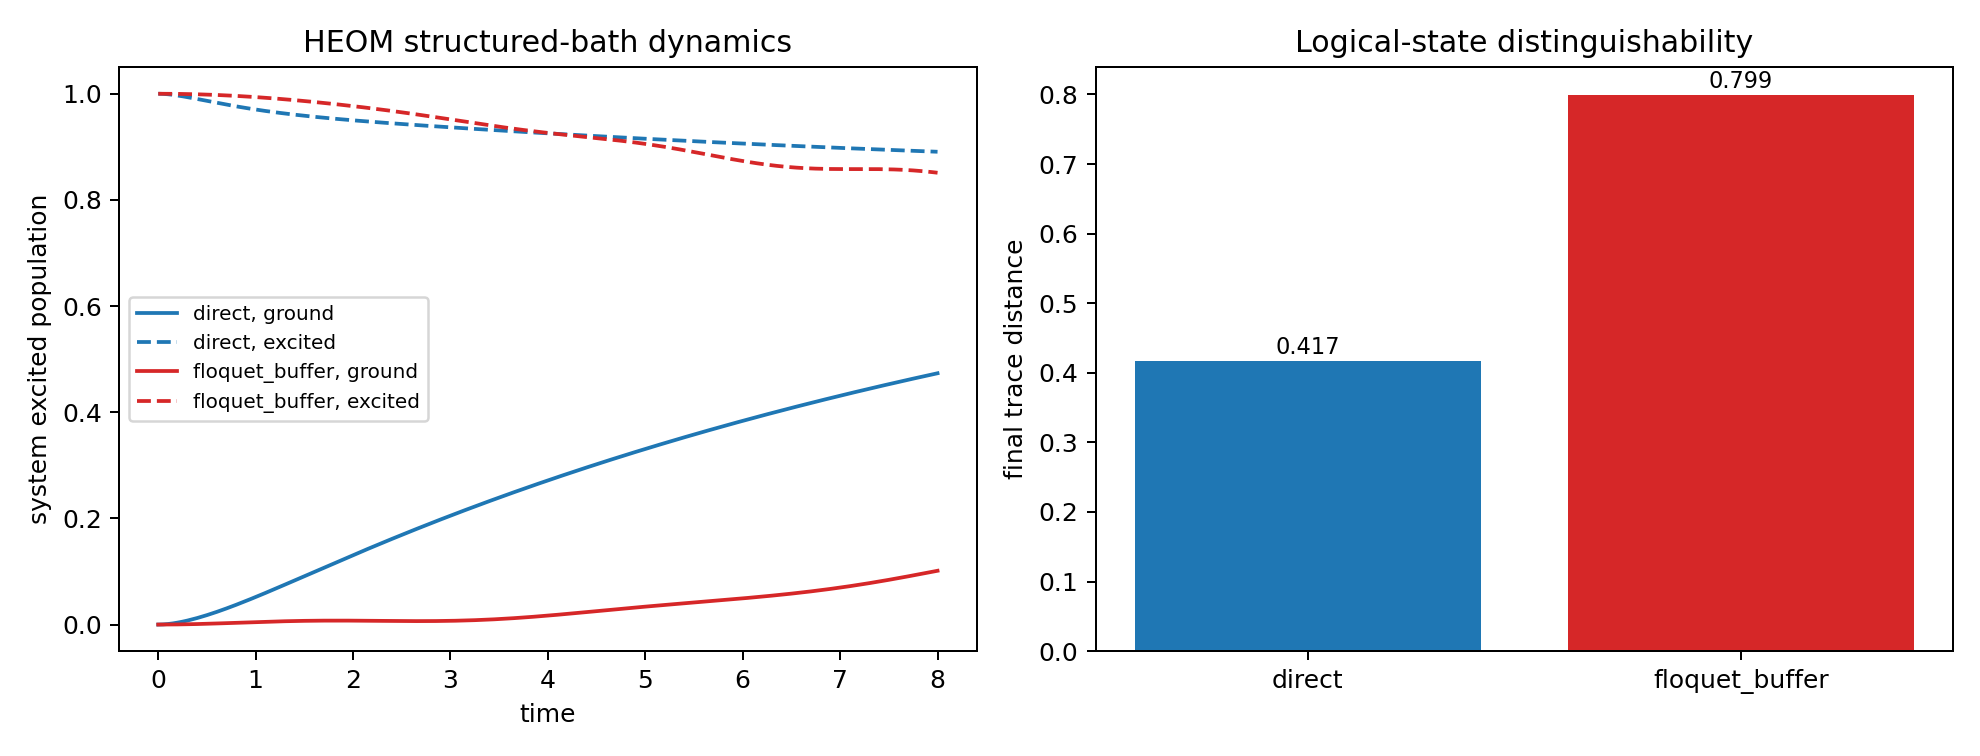
\includegraphics[width=0.82\linewidth]{heom_validation.png}
\caption{HEOM structured-bath validation of the output stage. The
Floquet-buffered branch preserves a larger final distinguishability
between the two logical initial states than the direct structured-bath
contact at the same bath parameters.}
\label{fig:heom-validation}
\end{figure}

\paragraph{HEOM depth scaling and exact-state MPS representability.}
The HEOM hierarchy was also swept over depths $N_{\mathrm{tier}}=2,3,4,5$
on a shortened scaling run. At depth $4$ the direct structured subsystem
has $D=0.522348$ with depth--5 drift $5.62\times10^{-8}$, while the
Floquet-buffered subsystem has $D=0.855945$ with drift
$4.46\times10^{-7}$. Thus the HEOM result is already stable by depths
$3$--$4$ for this benchmark.

For the preliminary tensor-network estimate, each reservoir was replaced
by a finite spin chain.  The state was propagated exactly and the bond
dimension needed to represent it as an MPS was inferred from its Schmidt
spectra; this was not an MPS time evolution. For bath-chain lengths
$L=2,\ldots,6$, the direct subsystem required maximum bond dimension
$\chi=2,4,4,6,6$, while the Floquet-buffered chain required
$\chi=4,4,6,6,6$. The buffered geometry therefore costs an extra local
site and a slightly larger small-$L$ bond, but it does not show runaway
bond growth in this benchmark. At $L=6$ the direct chain gives
$D=0.748064$ and the buffered chain gives $D=0.791114$.

\begin{figure}[H]\centering
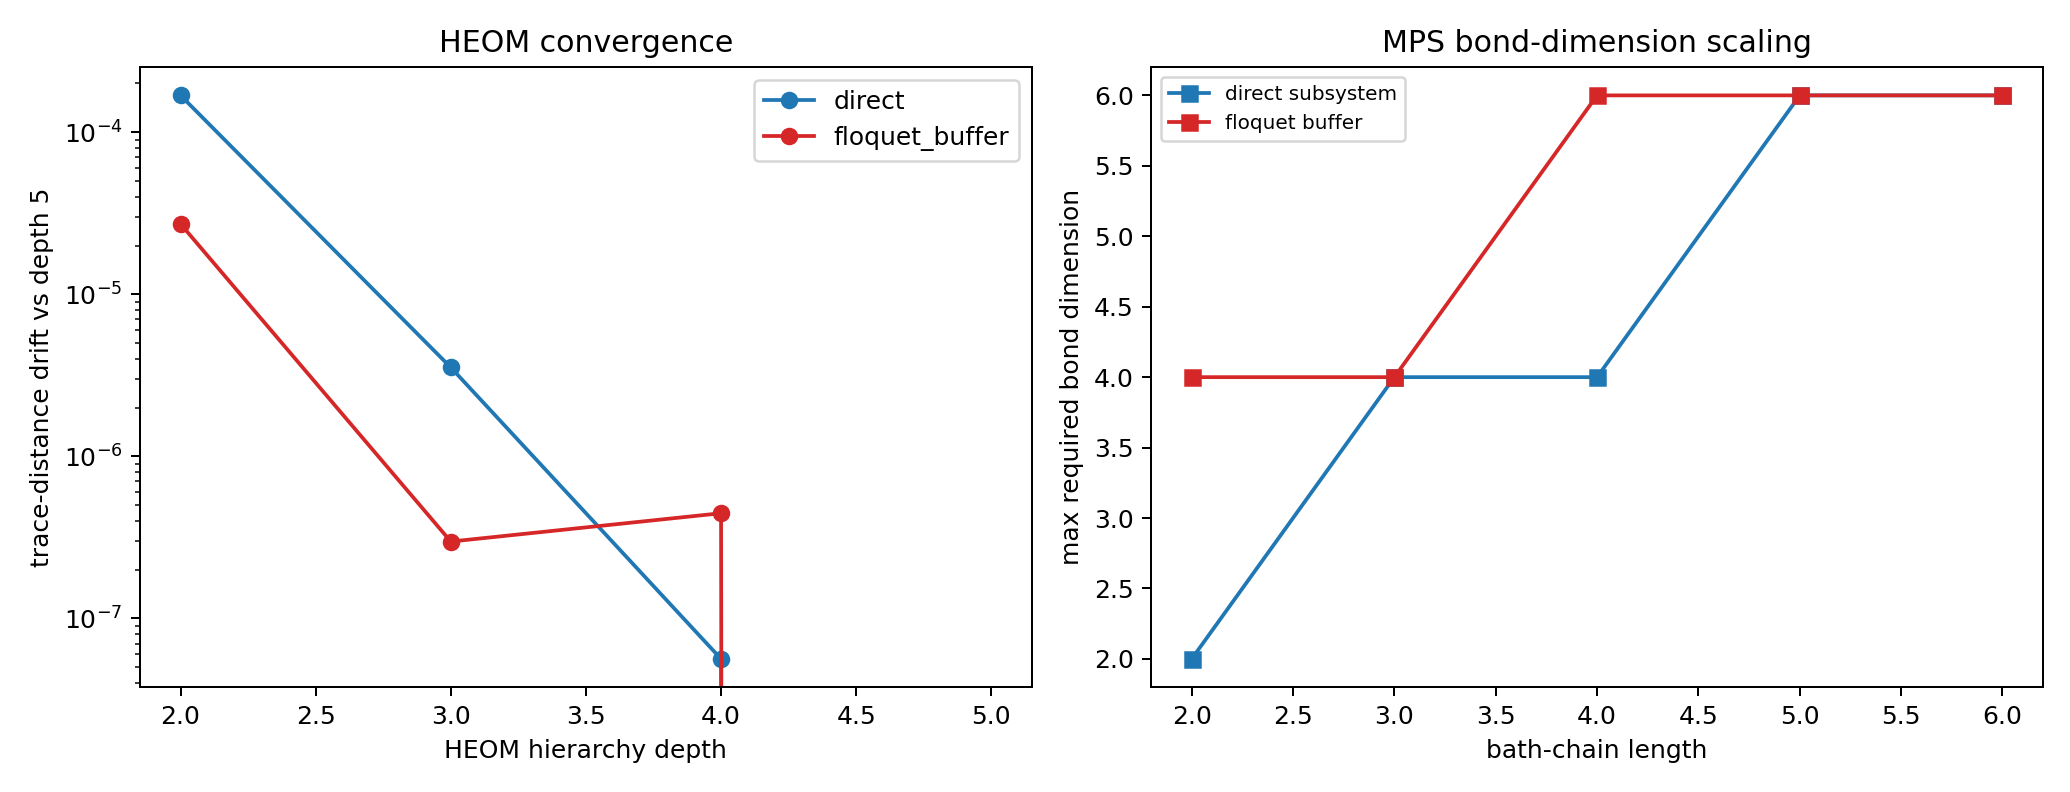
\includegraphics[width=0.86\linewidth]{heom_mps_scaling.png}
\caption{Scaling validation. Left: HEOM convergence versus hierarchy
depth, measured by trace-distance drift relative to depth $5$. Right:
exact-state MPS representability versus structured-bath chain length for
the direct subsystem and the Floquet-buffered subsystem.}
\label{fig:heom-mps-scaling}
\end{figure}

\paragraph{Energy/work comparison and practical interpretation.}
The direct structured-bath subsystem uses no external drive work:
$W_{\mathrm{drive}}=0$. It is therefore the lower-energy device if one
counts only externally supplied work. Its drawback is weaker logical
separation: in the HEOM depth--4 scaling run $D_{\mathrm{direct}}=0.522348$.
The Floquet-buffered subsystem consumes clock/drive work
$W_{\rm net}=-0.406107$, $W_+=0.038648$, and
$W_{\rm abs}=0.483403$, and has
$D_{\mathrm{buffer}}=0.855945$.  The conservative
work-throughput-per-distinguishability proxy is therefore
$W_{\rm abs}/D_{\mathrm{buffer}}=0.564759$. Thus the answer
to ``which uses less energy?'' is: the direct subsystem uses less external
energy, but the buffered subsystem buys stronger isolation and readout
distinguishability by spending drive work. The useful engineering
question is therefore not absolute work alone, but whether the improved
noise margin is worth the supplied AC power.

Practically, the architecture can be implemented in platforms that allow
tunable qubit gaps and engineered reservoirs. In superconducting circuits,
$C_z$ and $F_z$ can be transmon-like qubits or a qubit plus resonator,
the buffer gap can be modulated by flux or microwave driving, and the
structured bath can be an impedance-engineered transmission line or a
lossy resonator chain. In trapped ions or quantum dots, the same logic is
implemented by a driven auxiliary level coupled to phonon/electronic
reservoir modes. The experimental signature is simple: prepare the two
logical input states, run the direct and buffered devices to the same
readout time, measure the output populations or trace-distance proxy,
and compare the gain against calibrated drive power.

\paragraph{Broad HEOM Floquet phase sweep.}
To move beyond a single hand-picked point, the HEOM output-stage model was
swept over drive amplitude $A\in\{0,0.2,0.35,0.55\}$, drive frequency
$\Omega\in\{0.8,1.2,1.8\}$, system--buffer coupling
$g_{SF}\in\{0.04,0.08,0.14\}$, reorganization energy
$\lambda\in\{0.025,0.045,0.075\}$, and bath cutoff
$\gamma_c\in\{0.8,1.8,3.0\}$, giving $324$ buffered HEOM points at
hierarchy depth $3$. Of these, $284$ points improve the direct
structured-bath distinguishability and $229$ points satisfy the robust
criterion $D_{\mathrm{buffer}}\ge0.75$ with positive gain. The best
absolute-gain point is
\[
A=0.55,\quad \Omega=1.2,\quad g_{SF}=0.04,\quad
\lambda=0.075,\quad \gamma_c=0.8,
\]
with
$D_{\mathrm{direct}}=0.353784$,
$D_{\mathrm{buffer}}=0.977156$, and
$\Delta D=0.623372$.  The drive-power sign changes during the cycle, so
three distinct work quantities are retained:
\begin{equation}
 W_{\rm net}=\int_0^{t_f}P(t)\d t,\qquad
 W_{+}=\int_0^{t_f}\max[P(t),0]\d t,\qquad
 W_{\rm abs}=\int_0^{t_f}|P(t)|\d t .
 \label{eq:work-accounting}
\end{equation}
Here $W_{\rm net}$ permits ideal work recovery, $W_+$ counts energy
supplied to the quantum system, and $W_{\rm abs}$ is the conservative
cycle-throughput proxy when neither sign of power is assumed free.  At
the best-gain point these are
$W_{\rm net}=-0.539063$, $W_+=0.010179$, and
$W_{\rm abs}=0.559420$, giving
$\Delta D/W_{\rm abs}=1.114318$.  This correction matters: taking only
$|W_{\rm net}|$ can produce a false near-zero cost through cancellation.
The best driven point under the conservative ratio is
$A=0.2,\Omega=0.8,g_{SF}=0.04,\lambda=0.075,\gamma_c=0.8$, with
$D_{\mathrm{buffer}}=0.968718$, $\Delta D=0.614933$,
$W_{\rm abs}=0.090825$, and
$\Delta D/W_{\rm abs}=6.770543$.

\begin{figure}[H]\centering
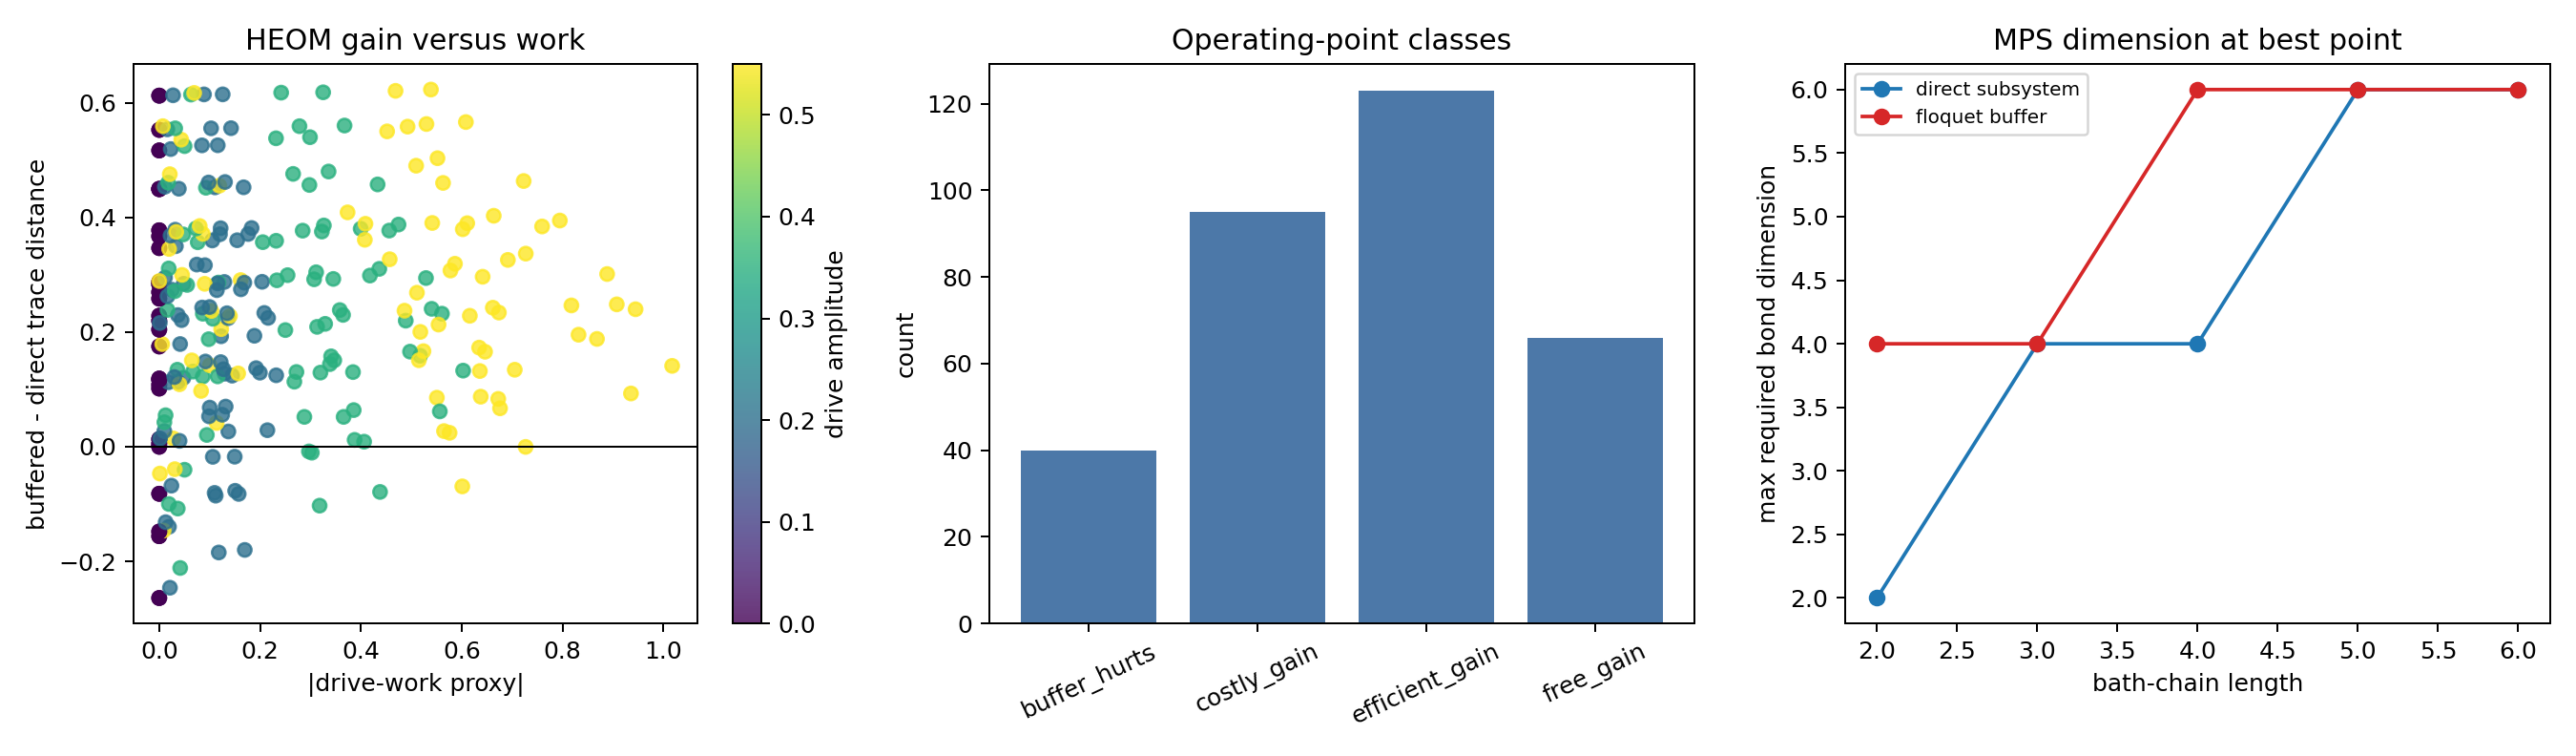
\includegraphics[width=0.92\linewidth]{heom_floquet_phase_summary.png}
\caption{Broad HEOM phase-sweep summary. The sweep compares output-stage
direct structured-bath contact against Floquet-buffered contact over
drive, coupling, and bath-memory parameters; the MPS panel shows the
bond-dimension estimate at the best-gain operating point.}
\label{fig:heom-phase-summary}
\end{figure}

\begin{figure}[H]\centering
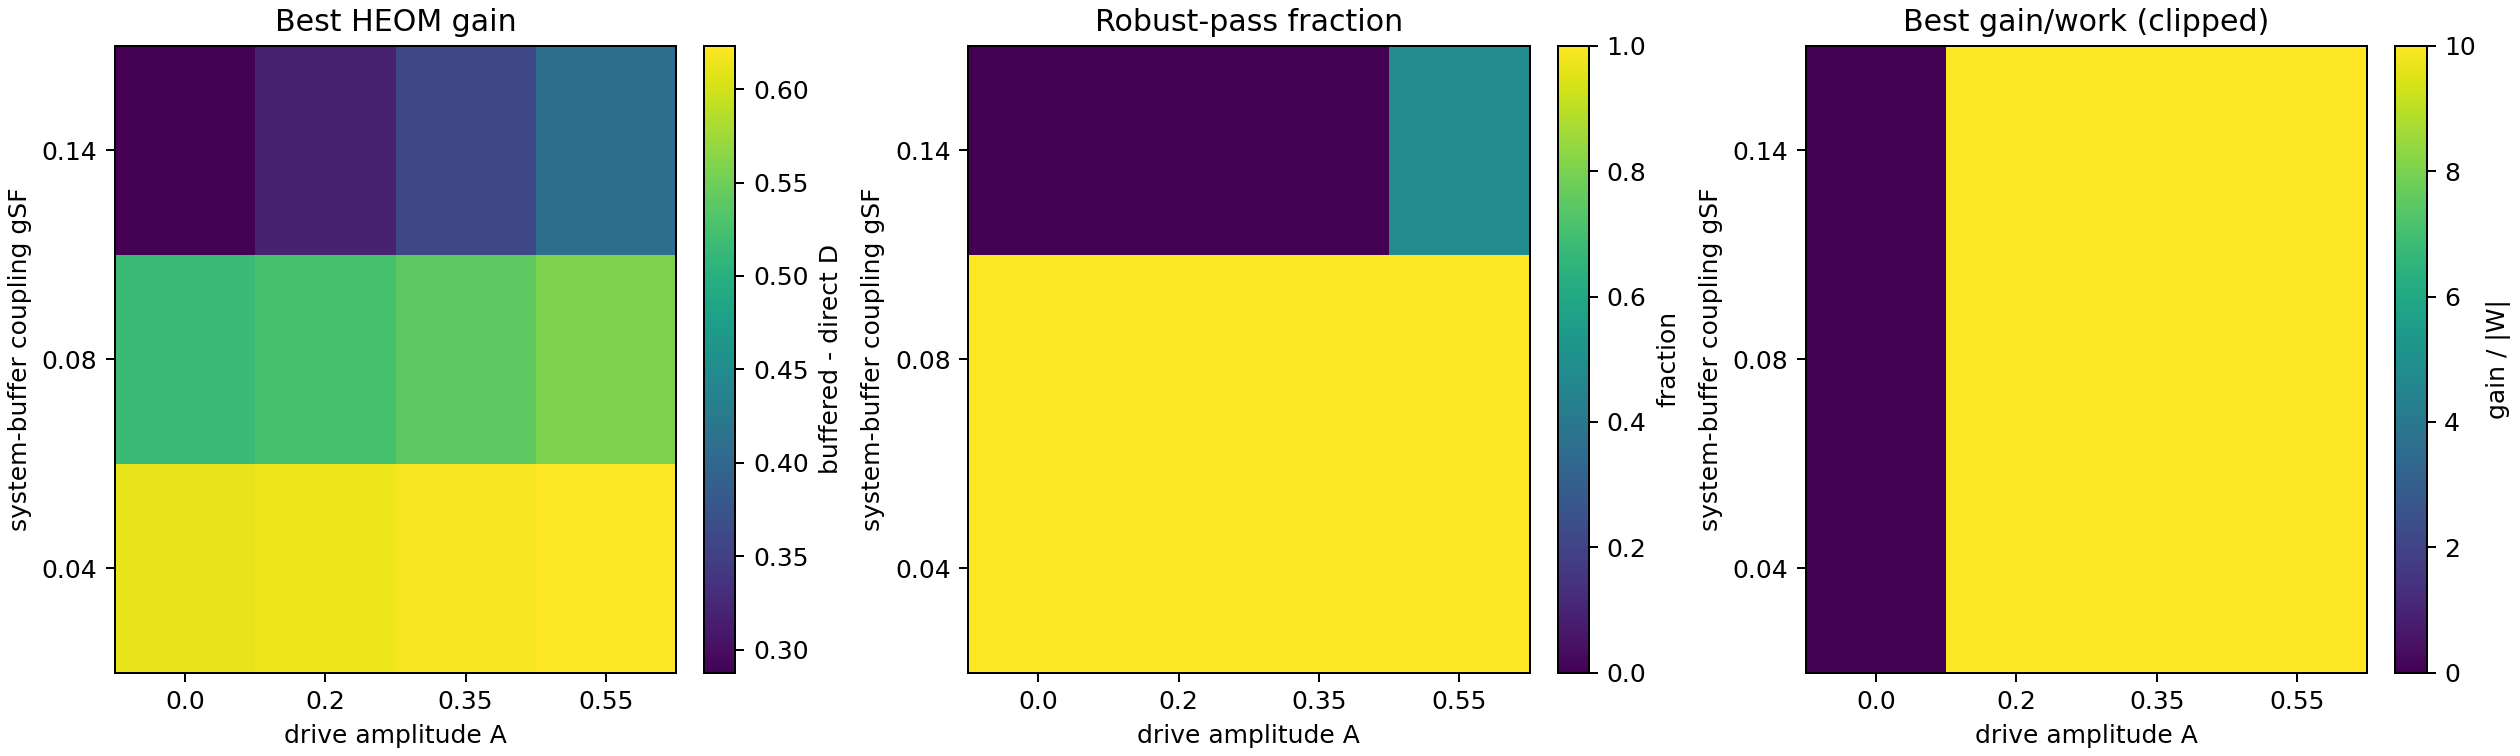
\includegraphics[width=0.92\linewidth]{heom_floquet_operating_regions.png}
\caption{HEOM operating regions compressed over bath parameters and drive
frequency. The panels show best gain, robust-pass fraction, and clipped
gain/work over drive amplitude and system--buffer coupling.}
\label{fig:heom-operating-regions}
\end{figure}

\begin{figure}[H]\centering
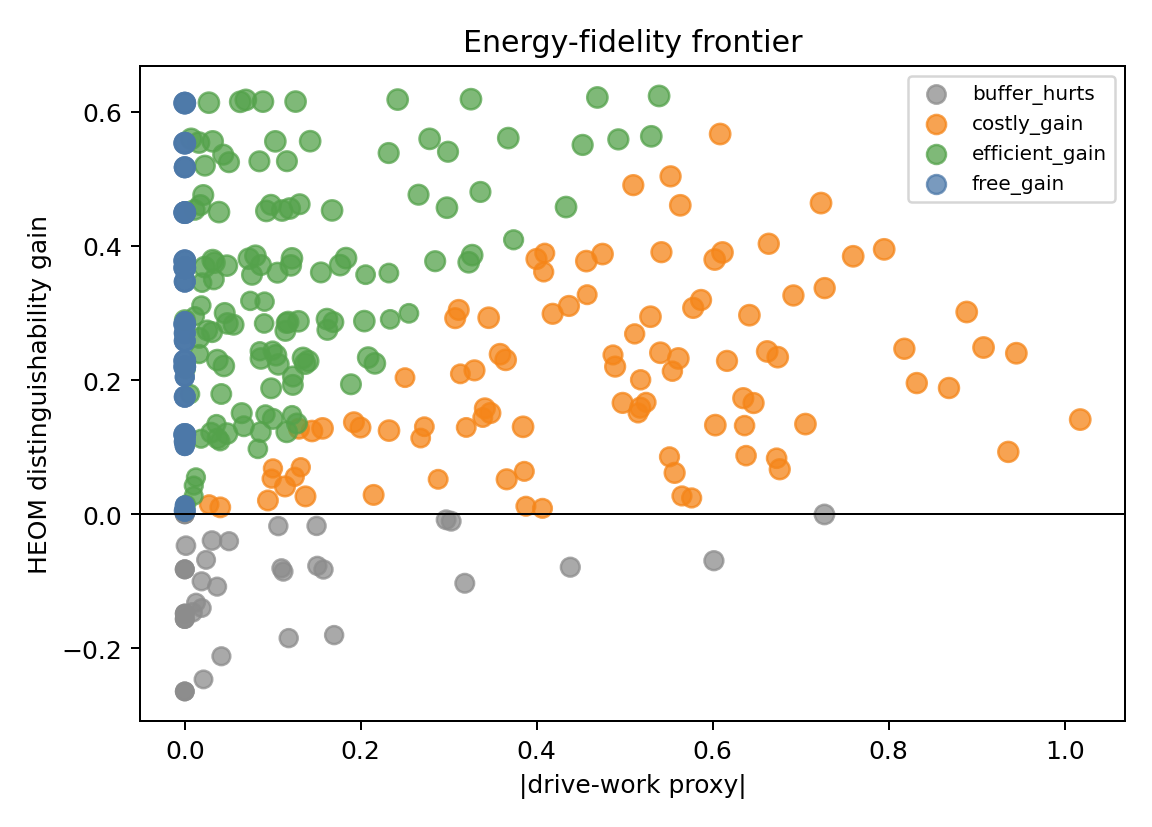
\includegraphics[width=0.68\linewidth]{heom_energy_fidelity_frontier.png}
\caption{Energy--fidelity frontier from the HEOM phase sweep. Direct
operation has zero external drive work; buffered operation spends
absolute drive-work throughput to gain output distinguishability. Marker
size scales with buffered final distinguishability.}
\label{fig:heom-energy-frontier}
\end{figure}

\paragraph{Six-state HEOM channel tomography.}
A two-state truth-table test probes only one diameter of the Bloch sphere.
For a genuine channel test we propagate the six Pauli eigenstates
$\rho_{\pm j}=(I\pm\sigma_j)/2$ for $j=x,y,z$.  Linearity then reconstructs
the action of the channel $\mathcal{E}$ without an ancilla:
\begin{equation}
 \mathcal{E}(I)=\mathcal{E}(\rho_{+z})+\mathcal{E}(\rho_{-z}),\qquad
 \mathcal{E}(\sigma_j)=\mathcal{E}(\rho_{+j})-\mathcal{E}(\rho_{-j}).
 \label{eq:six-state-reconstruction}
\end{equation}
The Pauli-transfer matrix and normalized Choi matrix follow as
\begin{align}
 R_{\mu\nu}&=\frac12\Tr[\sigma_\mu\mathcal{E}(\sigma_\nu)],
 &
 J_{\mathcal{E}}&=\frac14\sum_{\nu=0}^{3}
 \mathcal{E}(\sigma_\nu)\otimes\sigma_\nu^{\mathsf T}.
 \label{eq:ptm-choi}
\end{align}
Trace preservation demands $R_{0\nu}=\delta_{0\nu}$ and complete
positivity demands $J_{\mathcal{E}}\succeq0$.  If
$M=(R_{ij})_{i,j=1}^{3}$ is the
Bloch block, the directional retention, unitarity, and volume contraction
are
\begin{equation}
 D_j=\frac12\norm{\mathcal{E}(\rho_{+j})-\mathcal{E}(\rho_{-j})}_1,\qquad
 u=\frac13\Tr(M^{\mathsf T}M),\qquad
 V=|\det M|.
 \label{eq:channel-retention}
\end{equation}
For a target unitary with Bloch rotation $O_U$, the average fidelity is
\begin{equation}
 F_{\rm avg}(U,\mathcal{E})
 =\frac{3+\Tr(O_U^{\mathsf T}M)}{6}.
 \label{eq:channel-average-fidelity}
\end{equation}
Maximizing this expression over $O_U\in SO(3)$ by the singular-value
decomposition of $M$ separates a correctable coherent frame rotation from
irreversible contraction.

At the best-gain point, the direct channel gives
$D_{\min}=0.353784$, $u=0.224019$, $V=0.092394$, and optimized-frame
$F_{\rm avg}=0.731302$.  The buffered channel gives
$D_{\min}=0.977156$, $u=0.969593$, $V=0.954637$, and optimized-frame
$F_{\rm avg}=0.992331$.  Its uncorrected identity fidelity is only
$0.757738$ because the off-diagonal PTM entries describe a large coherent
rotation; calibration removes that deterministic frame error.  Both Choi
matrices are positive at numerical precision
($\lambda_{\min}=6.75\times10^{-2}$ direct and
$2.37\times10^{-5}$ buffered), and both trace-preservation residuals are
below $9\times10^{-16}$.

\begin{figure}[H]\centering
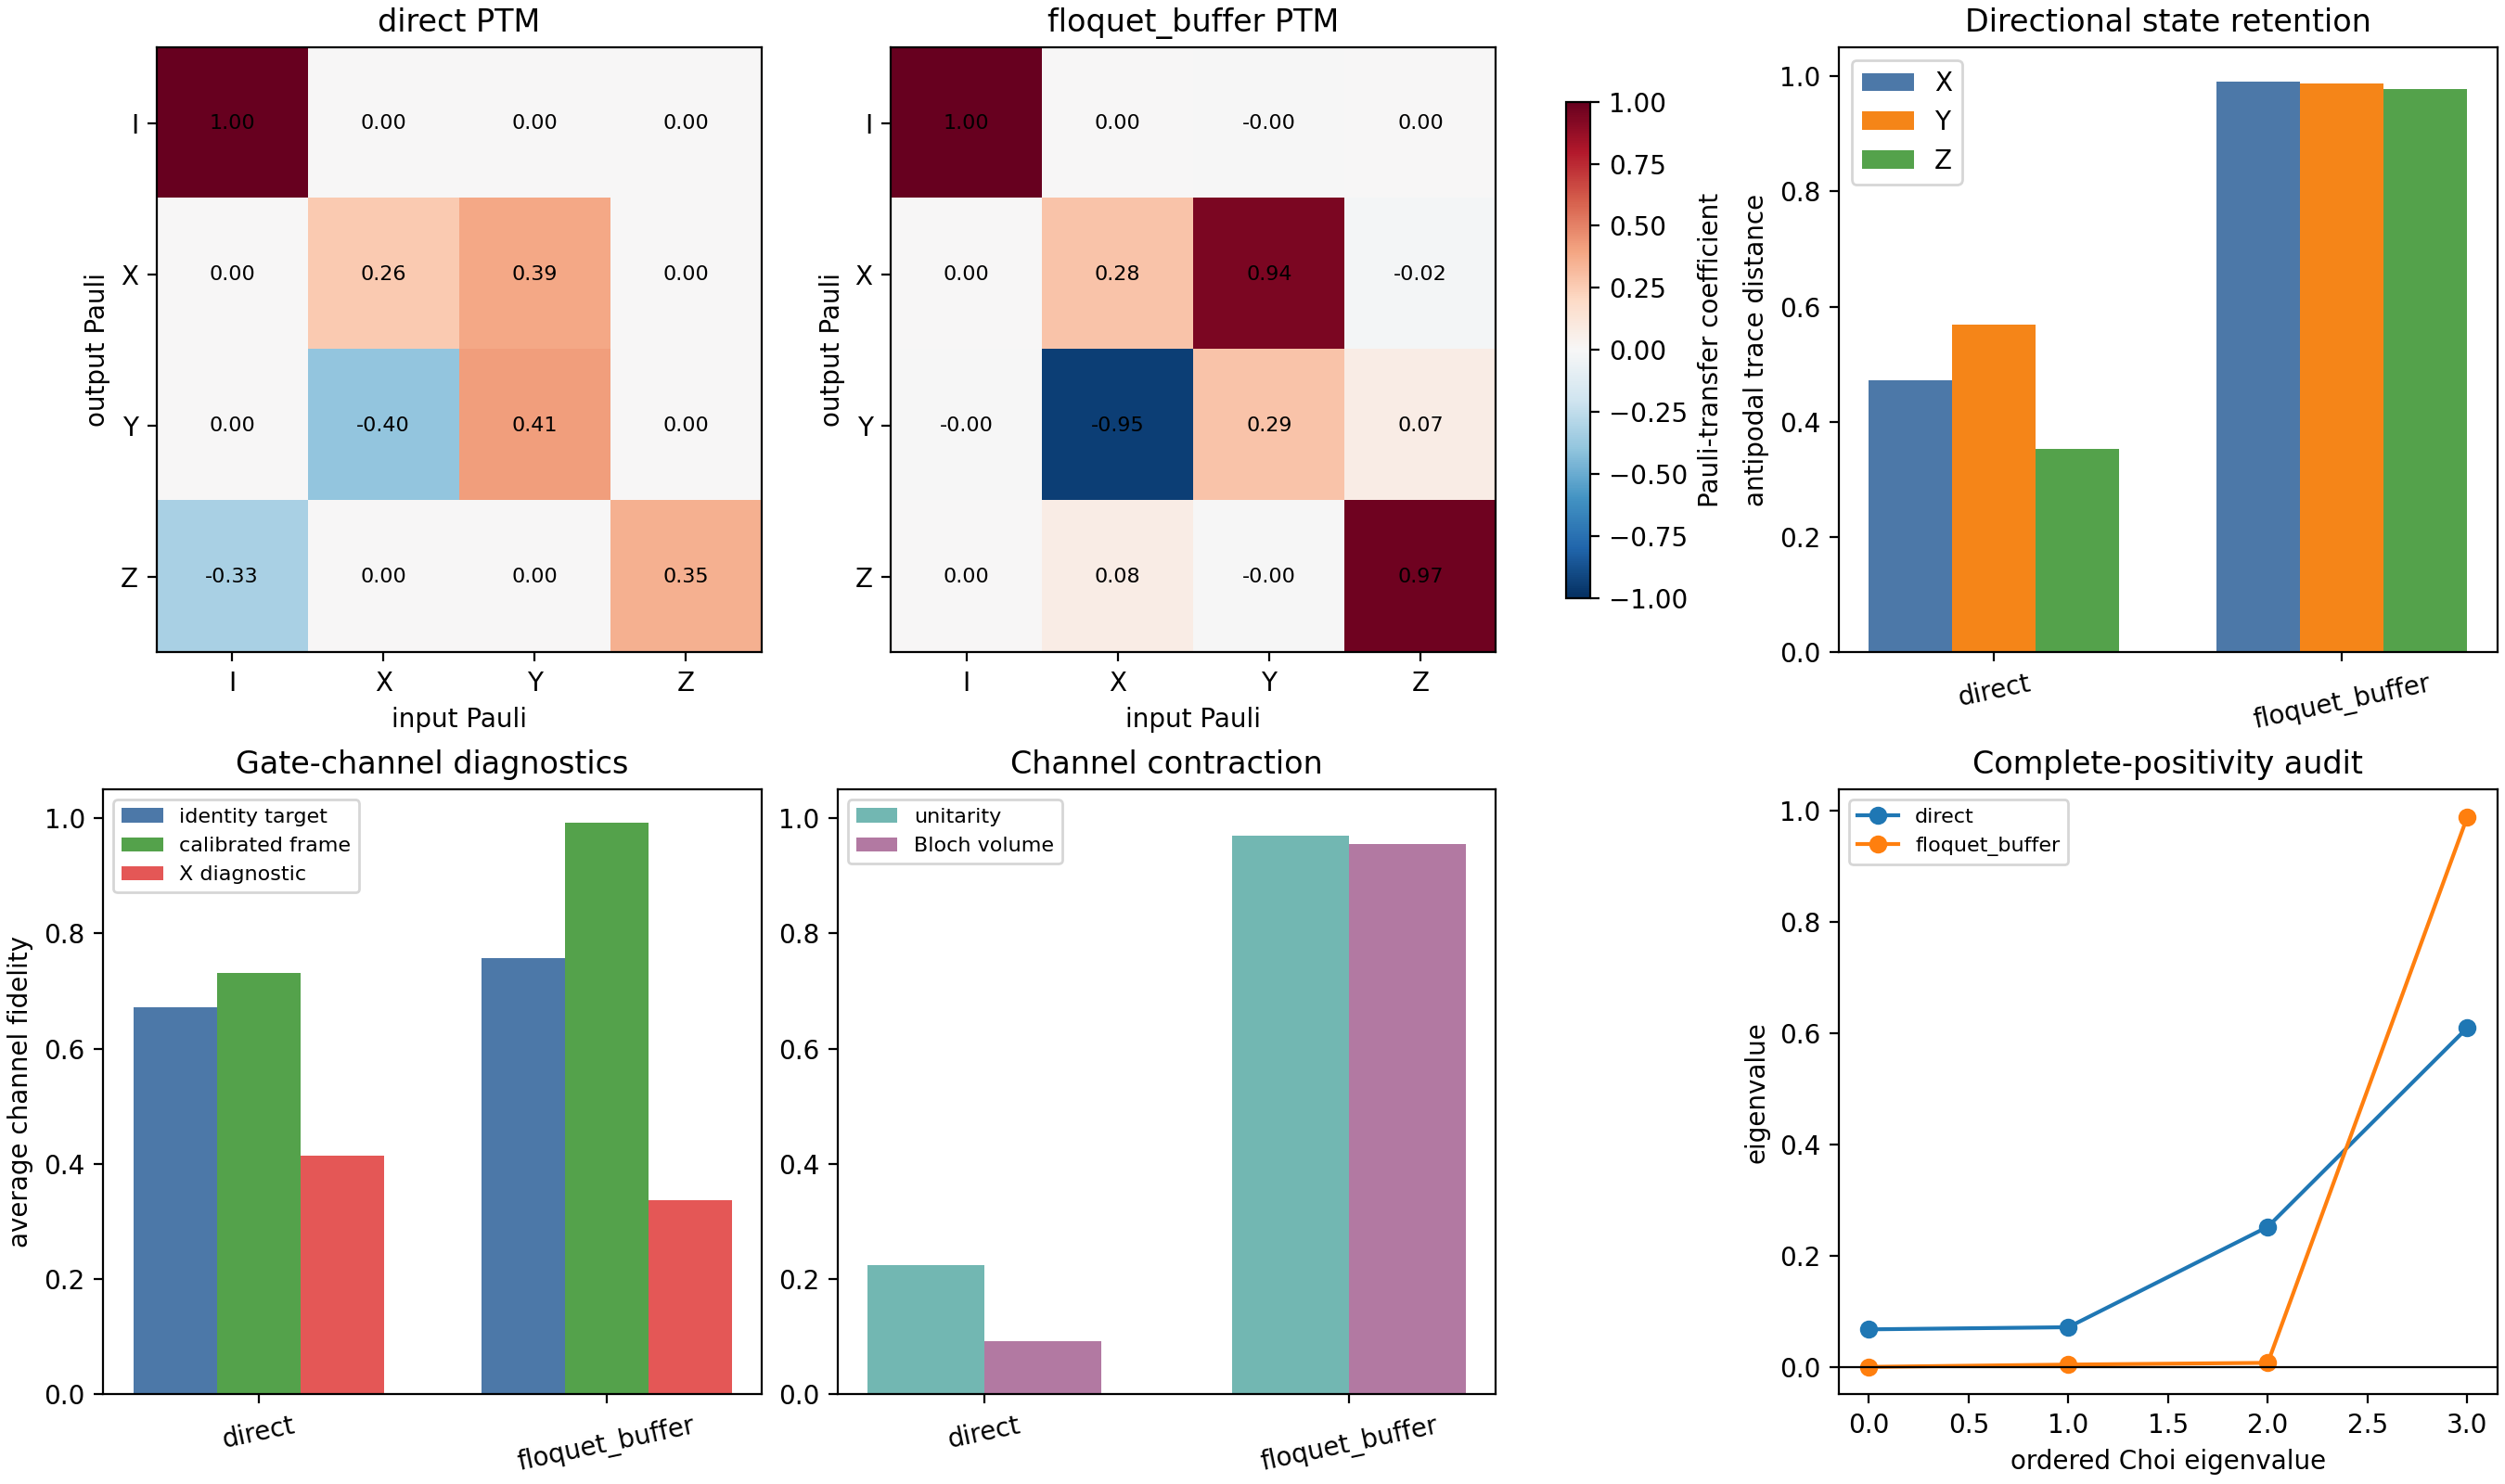
\includegraphics[width=0.98\linewidth]{heom_channel_tomography.png}
\caption{Six-state HEOM process tomography.  The PTMs expose coherent
rotation and irreversible contraction separately; the remaining panels
compare directional retention, raw and calibrated average fidelity,
unitarity, Bloch-volume contraction, and Choi positivity.}
\label{fig:heom-channel-tomography}
\end{figure}

\paragraph{Information backflow and cancellation-safe power.}
For any initial pair, contractivity of a CP-divisible map requires
$\dot D(t)\le0$.  The Breuer--Laine--Piilo measure is
\begin{equation}
 \mathcal{N}_{\rm BLP}=\max_{\rho_1,\rho_2}
 \int_{\dot D>0}\dot D[\rho_1(t),\rho_2(t)]\d t .
 \label{eq:blp-measure}
\end{equation}
We do not claim the continuous maximization in
Eq.~\eqref{eq:blp-measure}; summing positive increments for the three
Pauli-antipodal pairs gives a reproducible lower bound.  It is
$0.021490$ for direct contact and $3.38\times10^{-4}$ for the buffer.
Thus the buffer advantage here is not caused by stronger information
backflow.  It comes from spectral isolation: the integrated $z$-axis
distinguishability increases from $3.07861$ to $4.95044$ while sampled
backflow decreases.  Figure~\ref{fig:heom-backflow} also plots $P(t)$ and
the two non-cancelling cumulative work definitions from
Eq.~\eqref{eq:work-accounting}.

\begin{figure}[H]\centering
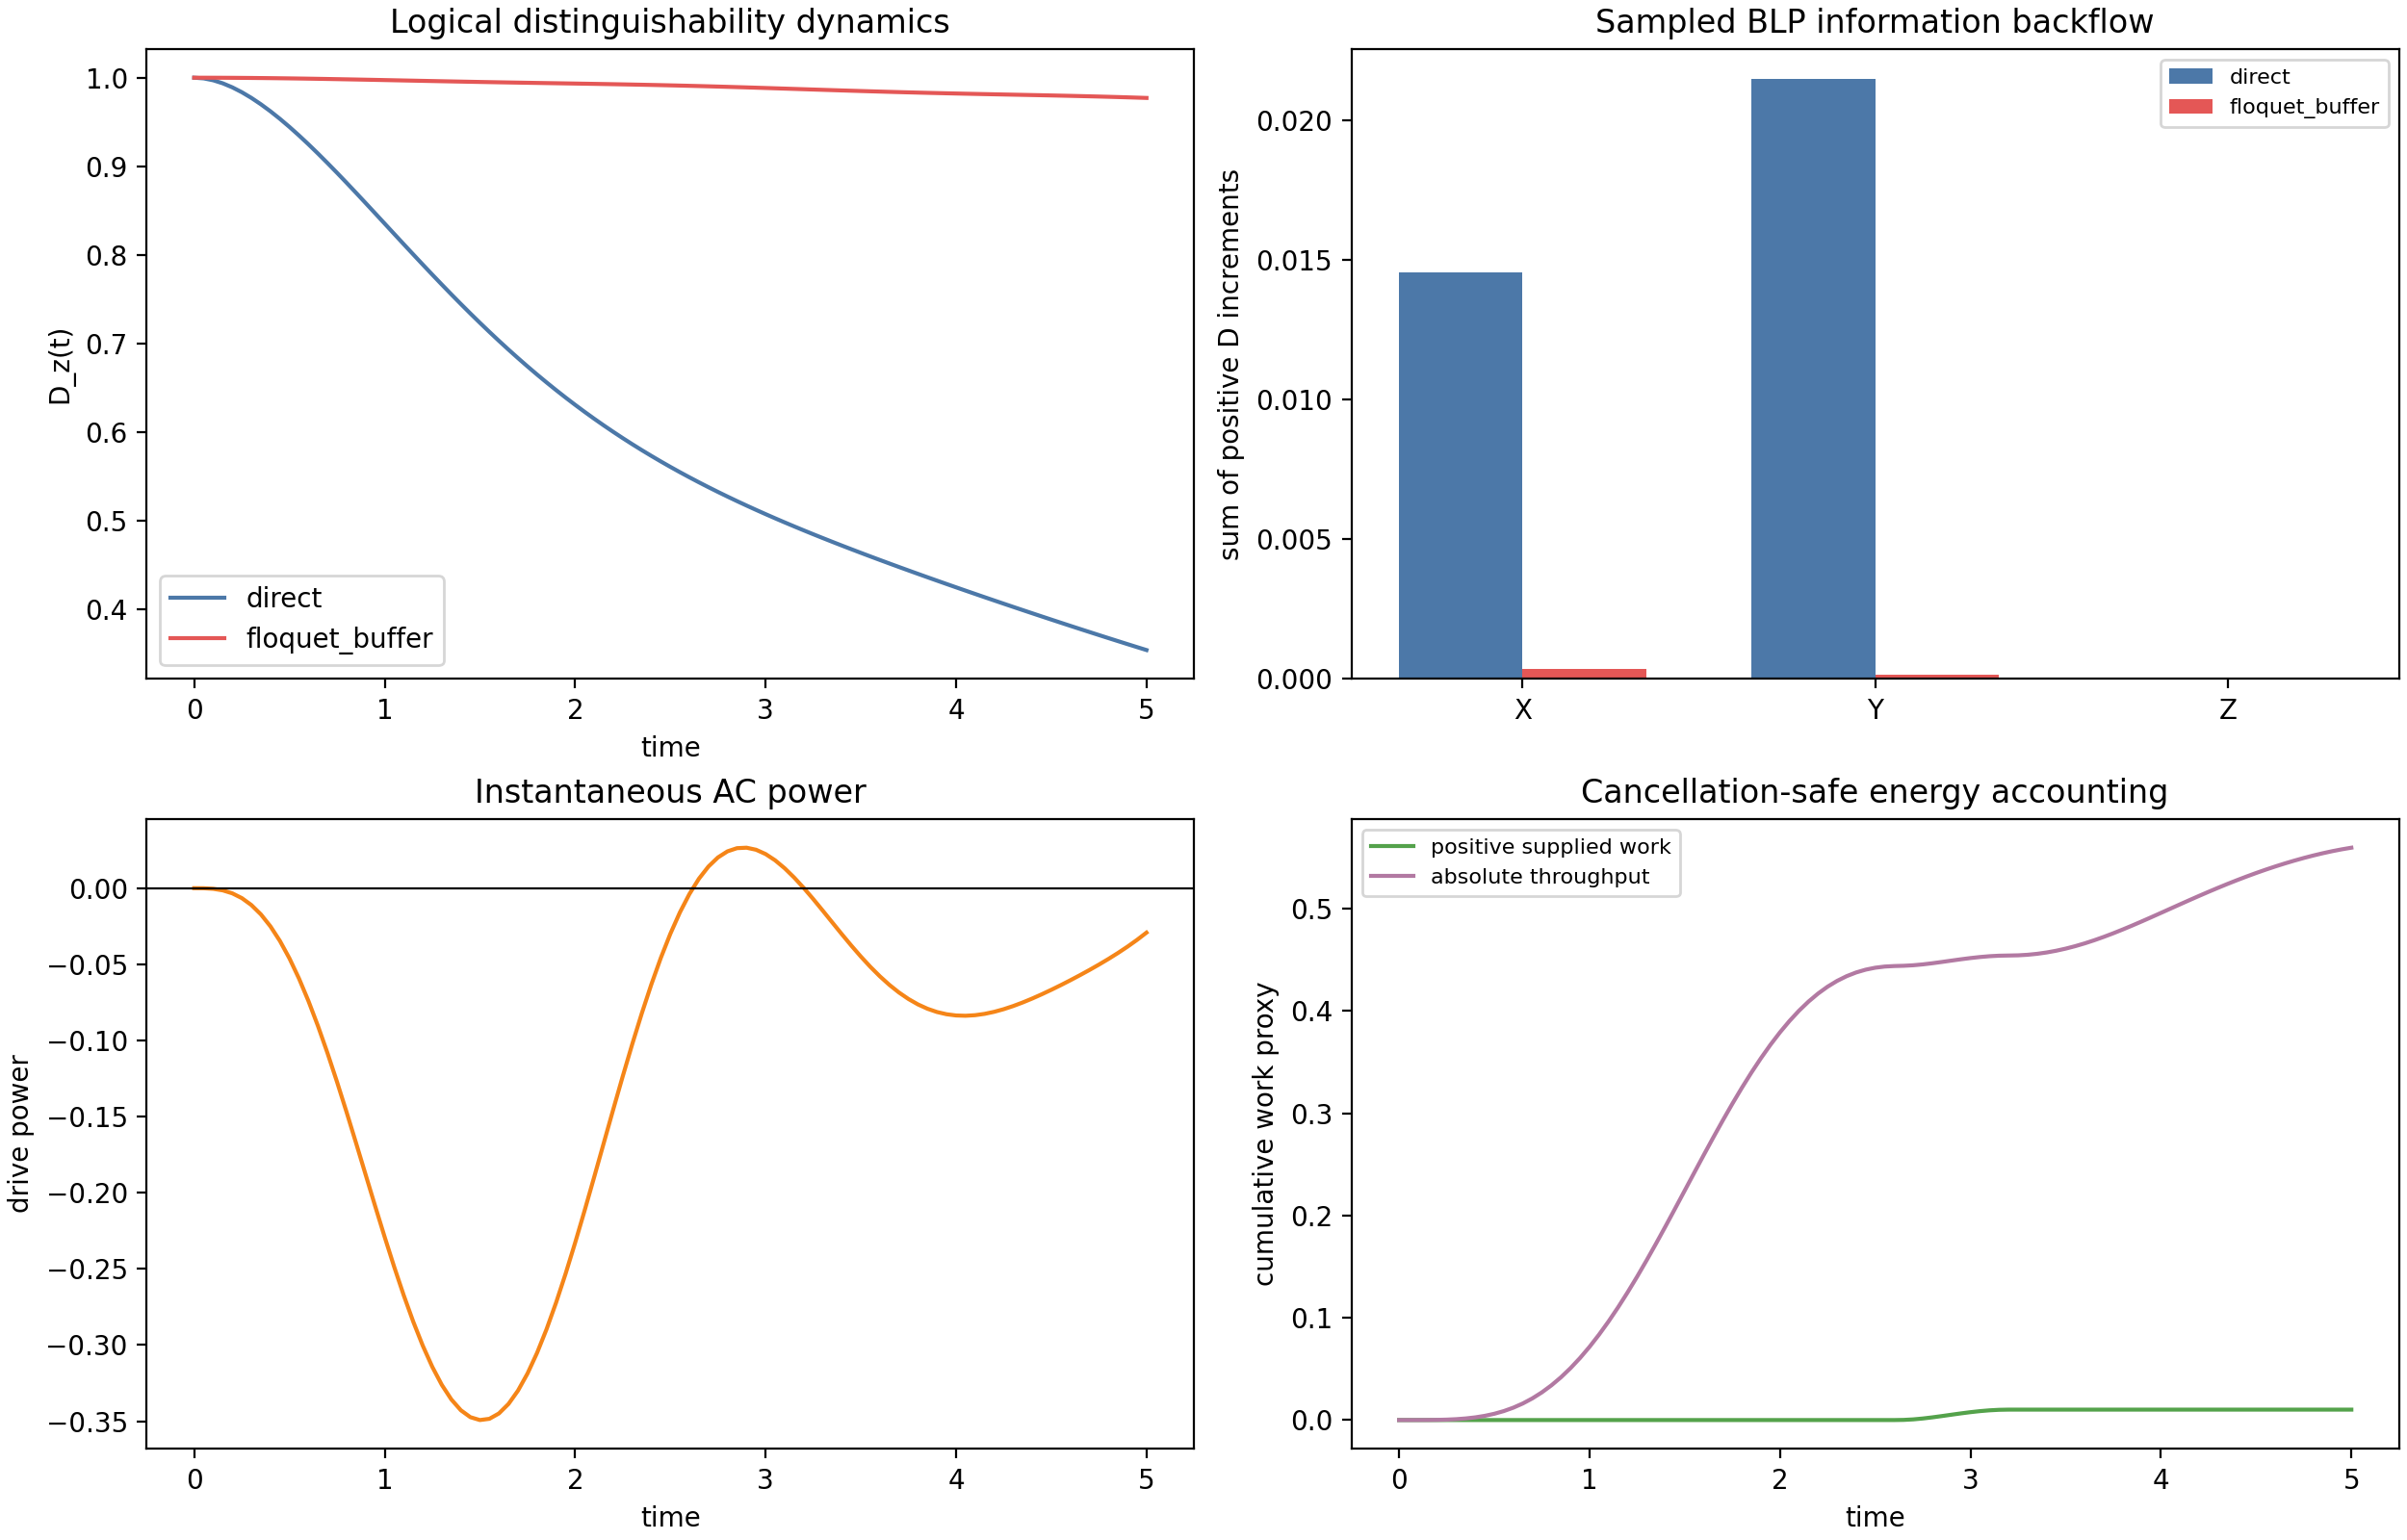
\includegraphics[width=0.94\linewidth]{heom_information_backflow.png}
\caption{HEOM distinguishability, sampled BLP information backflow, and
drive-power accounting.  Absolute throughput remains finite even when
positive and negative work nearly cancel in the net integral.}
\label{fig:heom-backflow}
\end{figure}

\paragraph{Readout phase and calibration uncertainty.}
The stroboscopic experiment was repeated for $16$ uniformly spaced drive
phases.  The gain remains in
$[0.618890,0.623372]$ with median $0.620839$, so the selected point does
not require phase-perfect readout.  A deterministic Latin-hypercube
ensemble then perturbed amplitude by $\pm10\%$, frequency by $\pm5\%$,
system--buffer coupling, reorganization energy, and bath cutoff by
$\pm15\%$, temperature by $\pm10\%$, and phase by $\pm\pi/6$.  All
$48/48$ HEOM samples satisfy $D_{\rm buffer}\ge0.75$ and $\Delta D>0$.
The median gain is $0.617616$ and the empirical $5$--$95\%$ interval is
$[0.567750,0.665942]$.  A standardized local linear fit ranks
reorganization energy, bath temperature, and bath cutoff as the dominant
uncertainties; this fit is a sensitivity summary, not a global surrogate
model.

\begin{figure}[H]\centering
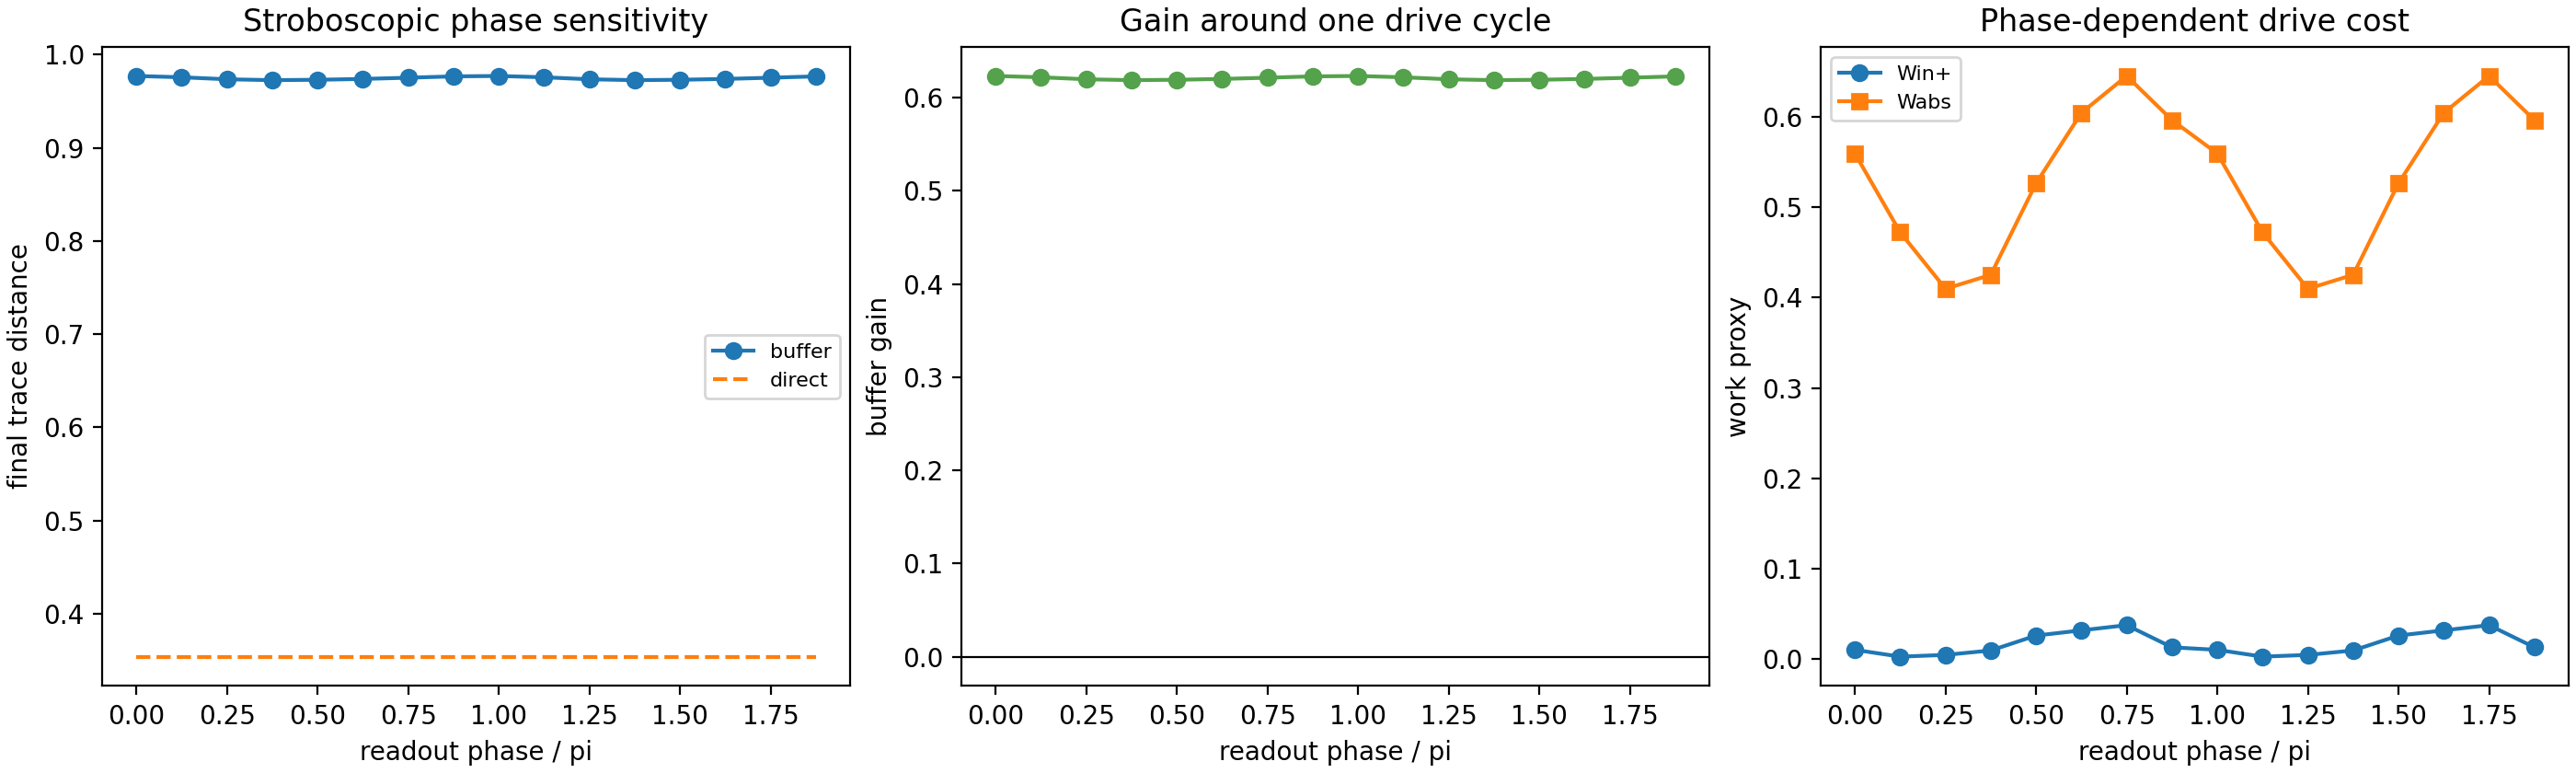
\includegraphics[width=0.94\linewidth]{heom_stroboscopic_phase.png}
\caption{Stroboscopic drive-phase sensitivity of final distinguishability,
buffer gain, and the two non-cancelling drive-work measures.}
\label{fig:heom-stroboscopic-phase}
\end{figure}

\begin{figure}[H]\centering
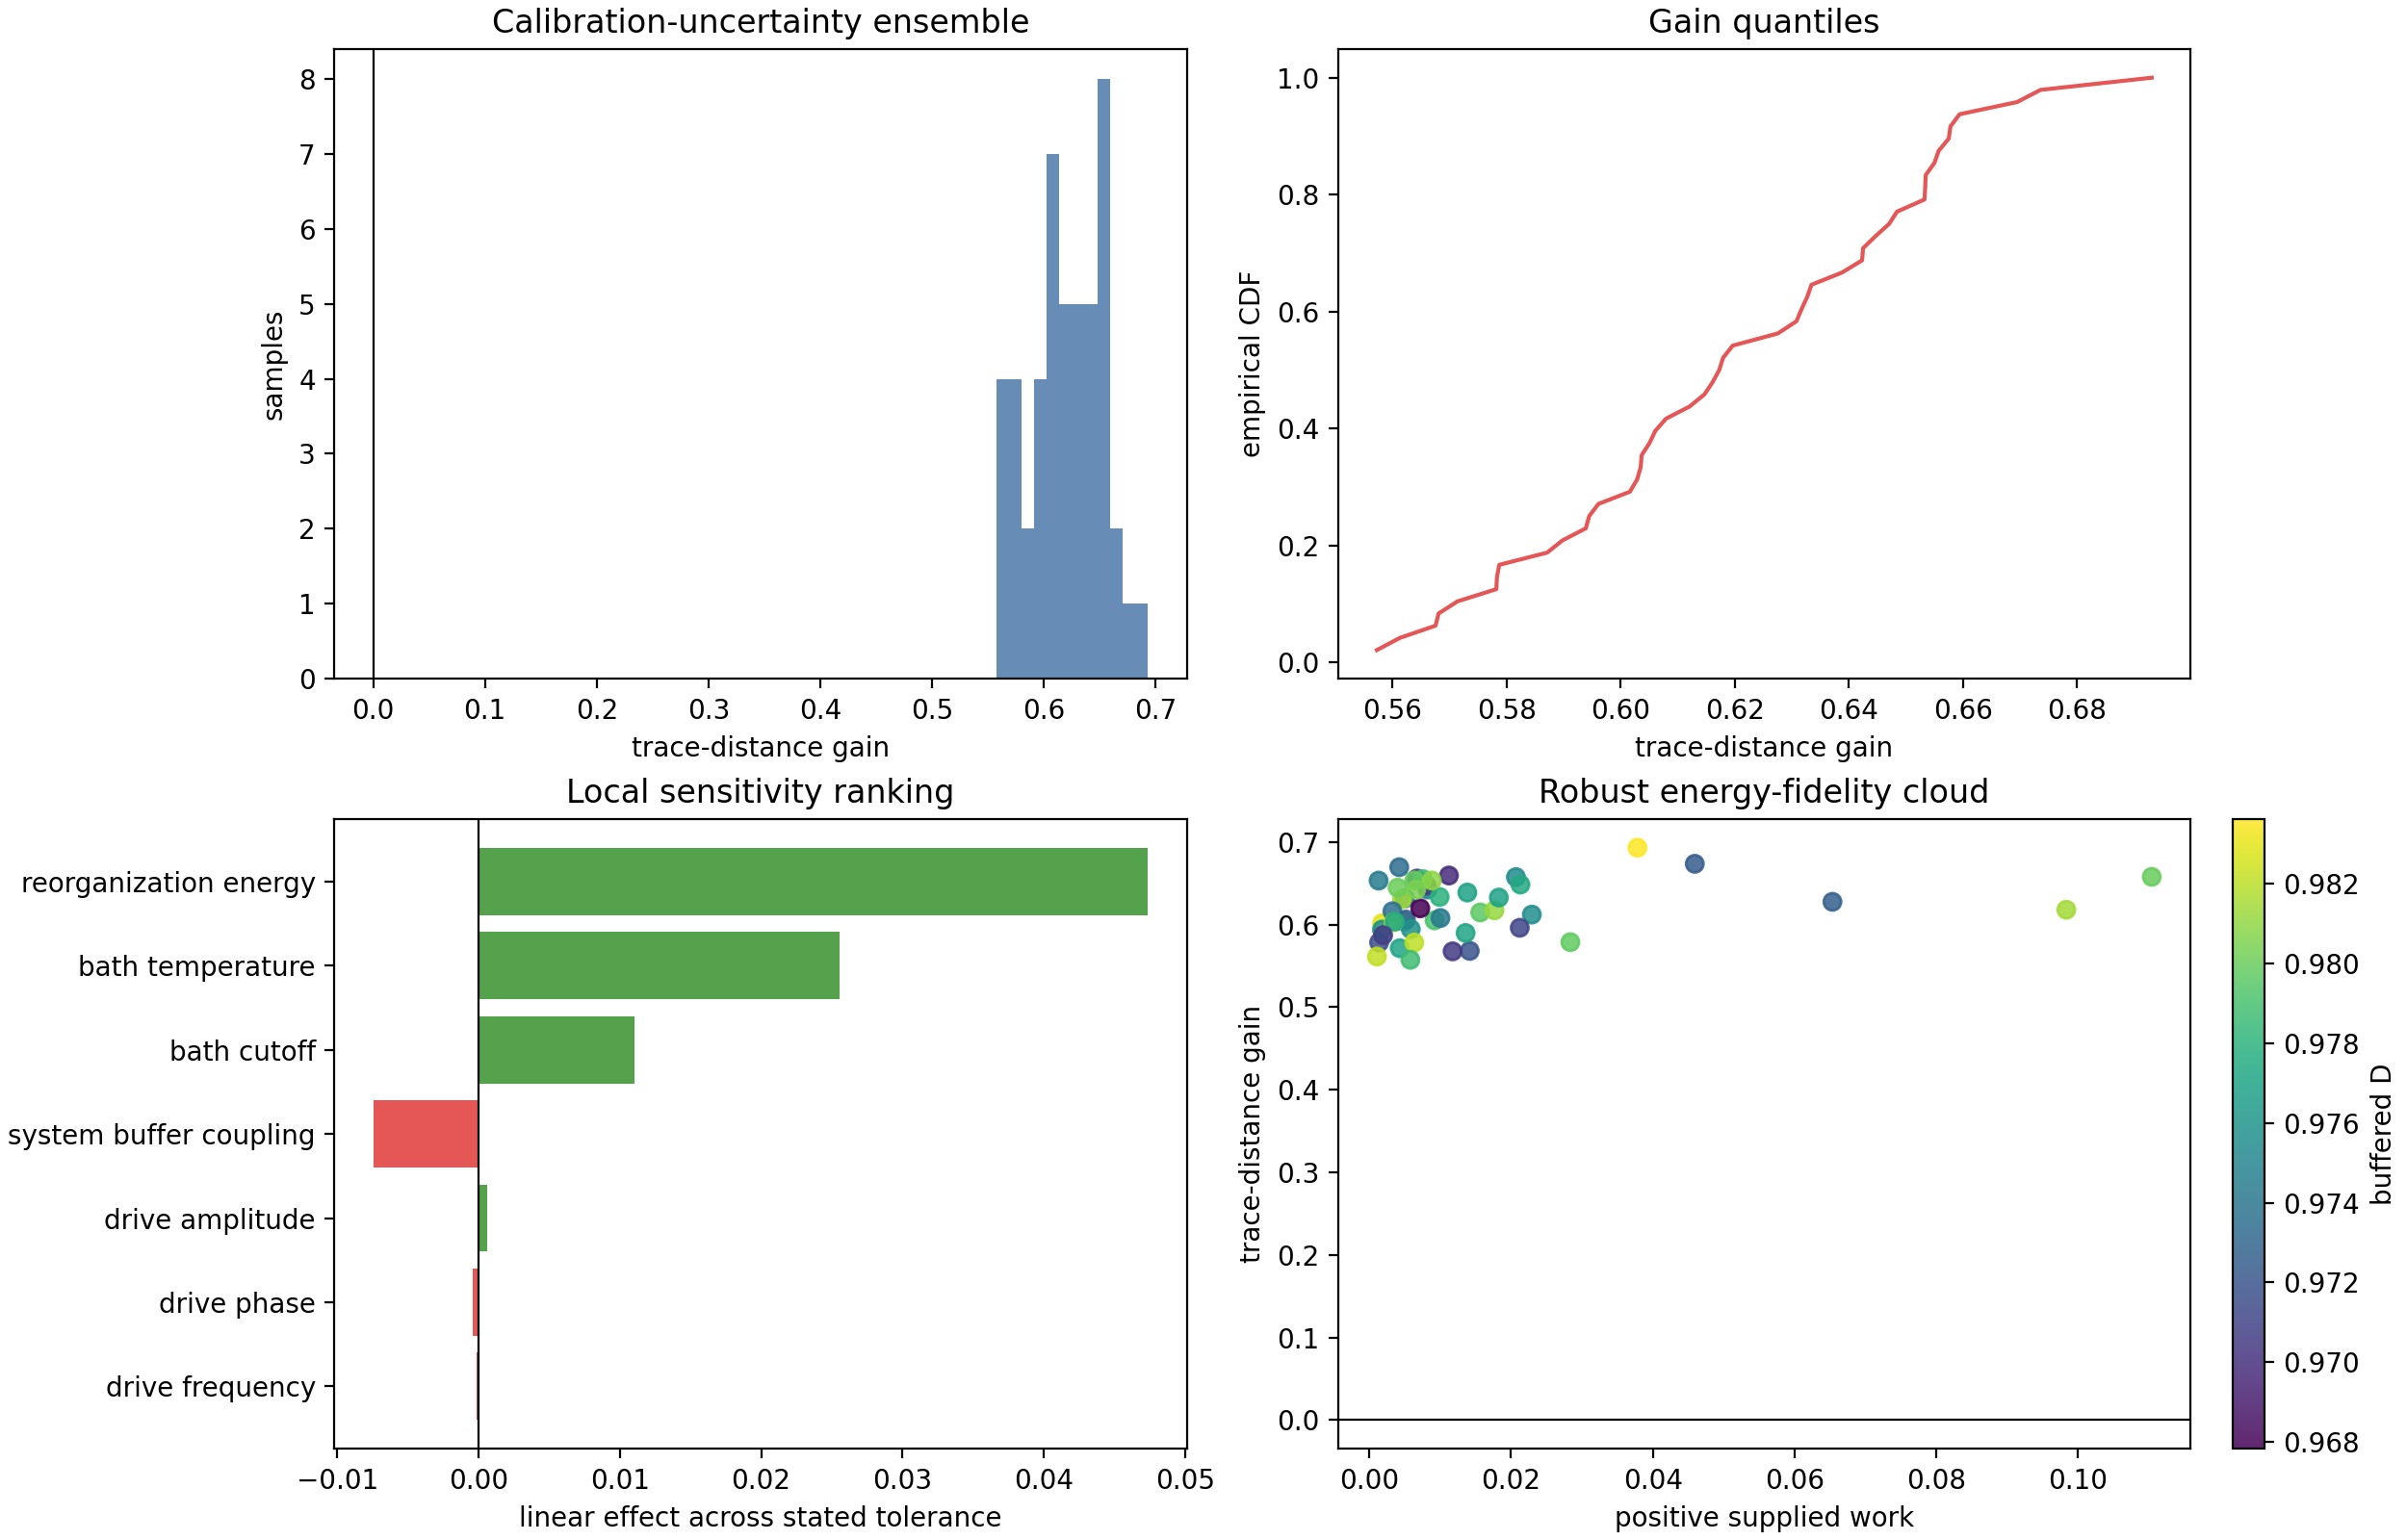
\includegraphics[width=0.94\linewidth]{heom_uncertainty_robustness.png}
\caption{Forty-eight-point HEOM calibration-uncertainty ensemble.  The
histogram and empirical CDF quantify gain variation; the signed effects
rank local sensitivities; the final panel shows the robust energy--fidelity
cloud.}
\label{fig:heom-uncertainty}
\end{figure}

\paragraph{Two-axis numerical convergence.}
Hierarchy depth alone is insufficient because the bath correlation
expansion also has to converge.  We therefore scan
$N_{\rm tier}=2,3,4$ and $N_k=1,2,3$, defining
\begin{equation}
 \delta_{N,K}=\max_{s\in\{0,1\}}
 D\!\left(\rho_s^{(N,K)}(t_f),\rho_s^{(4,3)}(t_f)\right).
 \label{eq:heom-two-axis-convergence}
\end{equation}
At the production setting $(N,K)=(3,2)$,
$\delta_{3,2}=3.289\times10^{-3}$ for direct contact and
$1.322\times10^{-4}$ for the buffered branch.  The refined result
therefore preserves the sign and scale of the $0.623$ buffer advantage by
a wide margin.

\begin{figure}[H]\centering
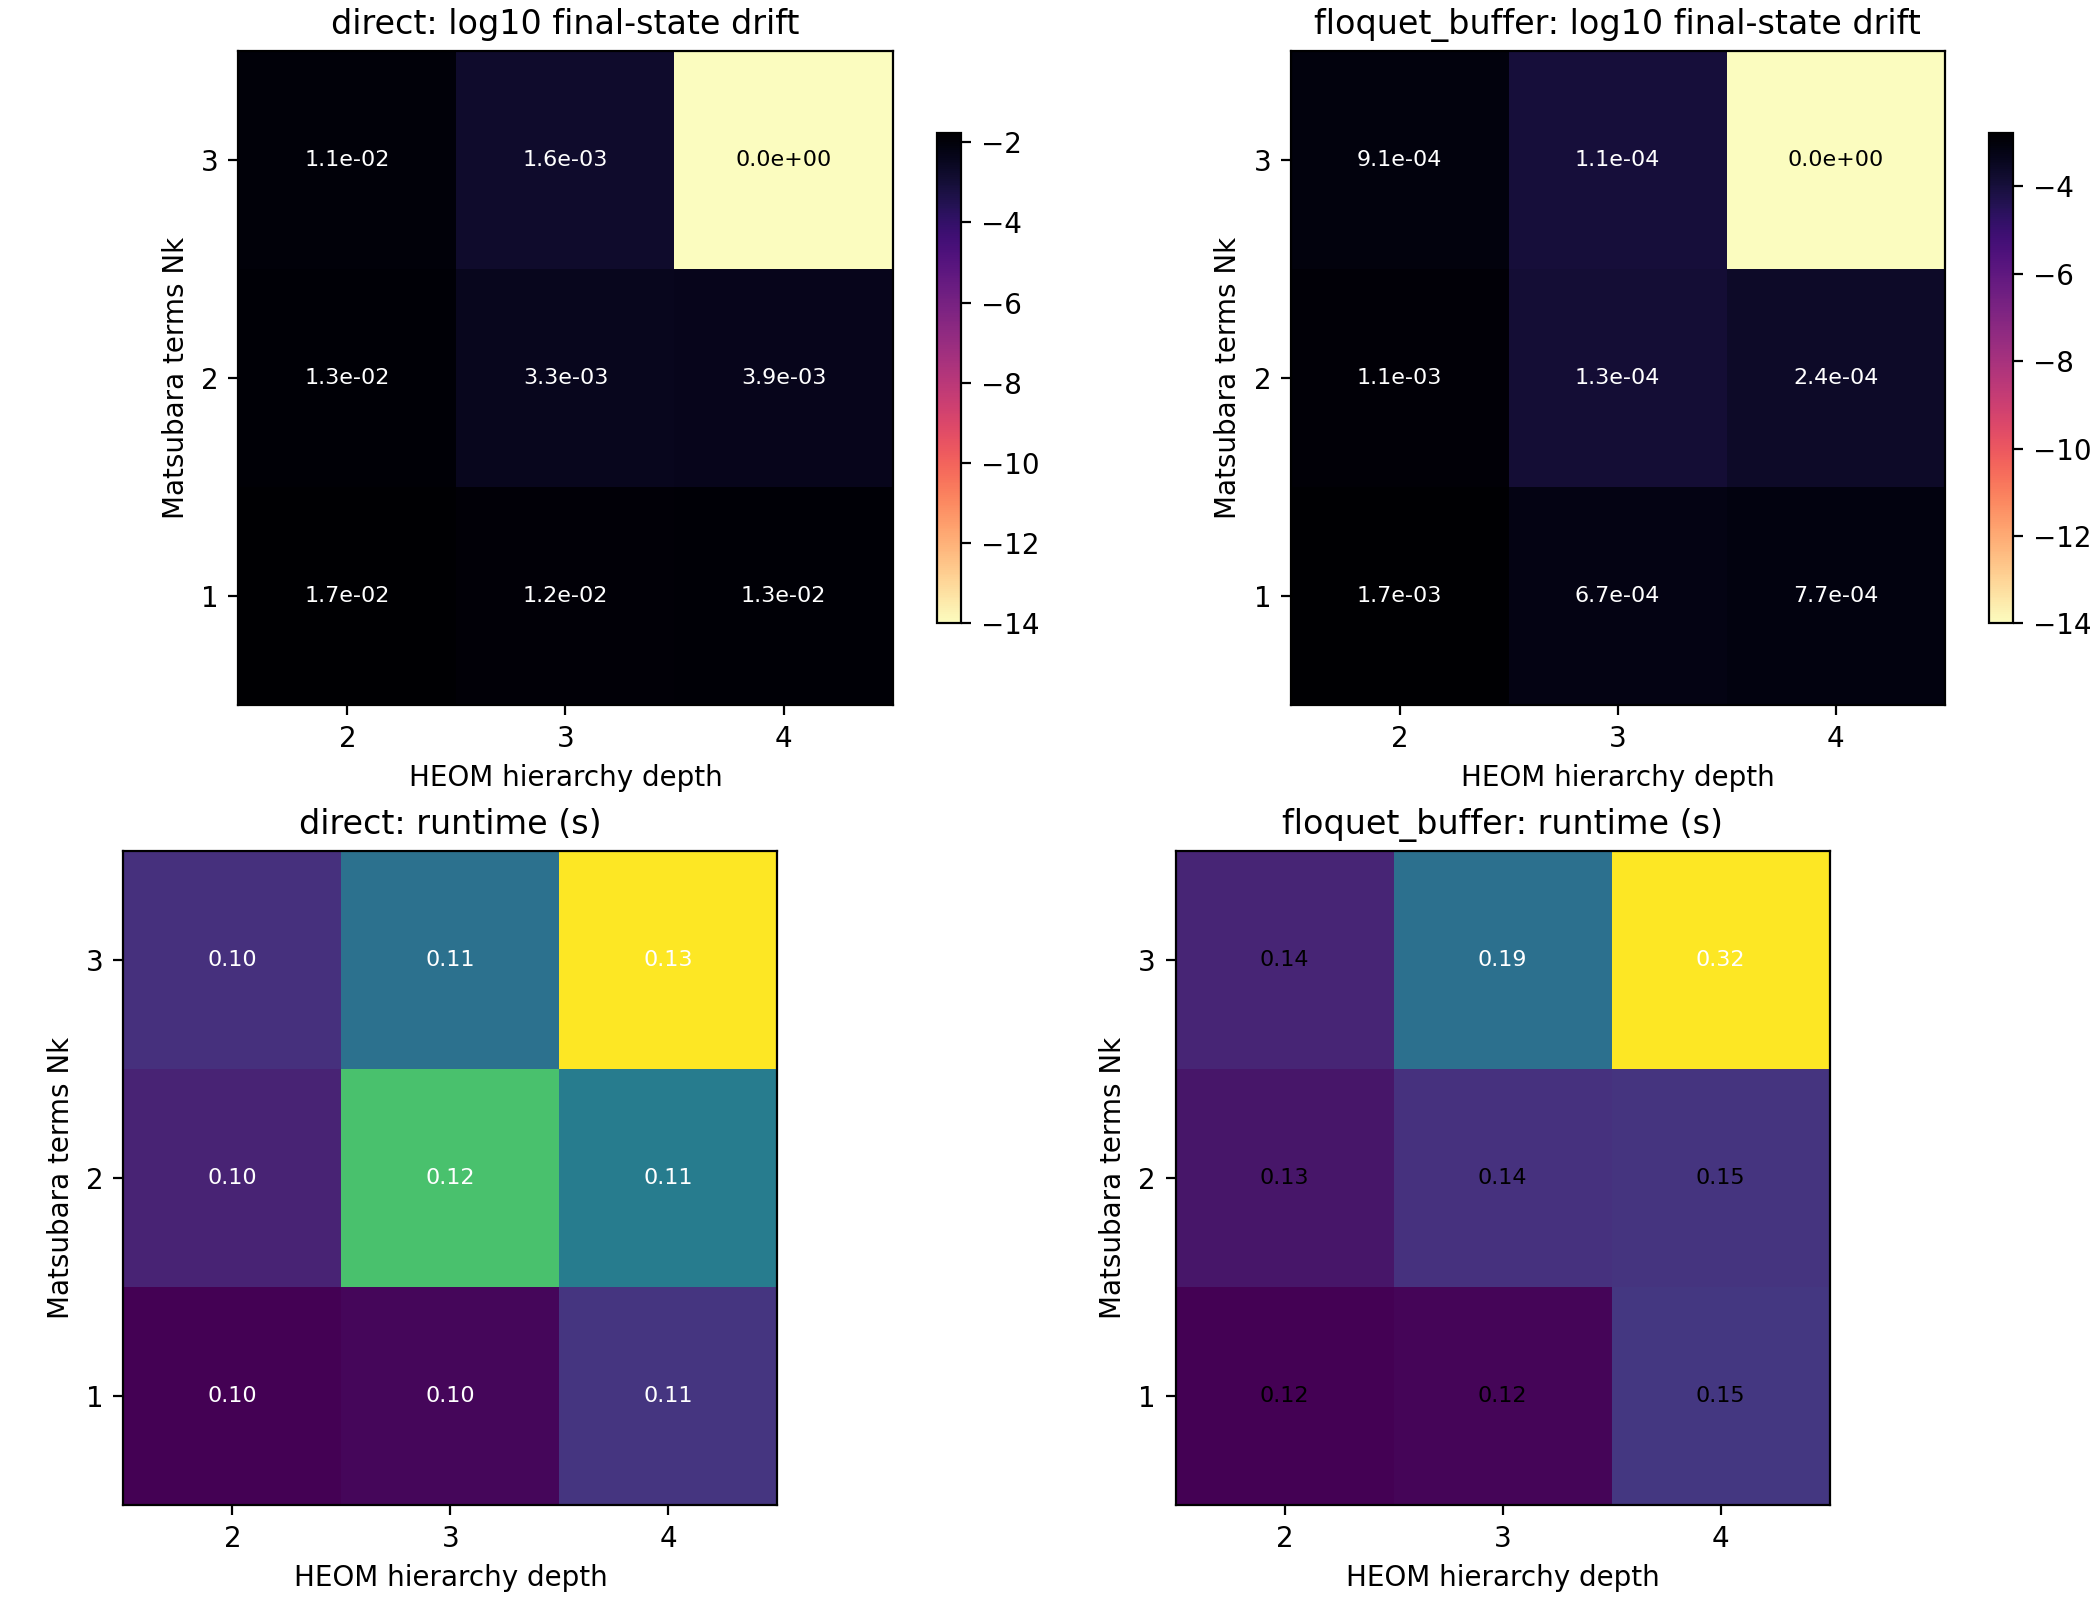
\includegraphics[width=0.88\linewidth]{heom_convergence_matrix.png}
\caption{Joint convergence in HEOM hierarchy depth and Matsubara expansion
order.  The upper panels show final-state trace-distance drift relative to
$(N_{\rm tier},N_k)=(4,3)$; the lower panels report measured runtime.}
\label{fig:heom-convergence-matrix}
\end{figure}

\begin{table}[H]
\centering\small
\caption{Approximations and scope limits specific to the advanced HEOM
experiments.}
\label{tab:advanced-heom-approximations}
\begin{tabularx}{\textwidth}{@{}l X X@{}}
\toprule
Item & What was assumed & How the claim is limited or checked \\
\midrule
Bath model & Drude--Lorentz spectral density represented by a finite
Matsubara expansion. & Both hierarchy depth and Matsubara order are
refined against $(4,3)$. \\
Channel reconstruction & Linearity is used to reconstruct a one-qubit
map from six Pauli eigenstates. & Choi positivity and trace preservation
are checked numerically. \\
BLP witness & Only the three Pauli-antipodal pairs are sampled. & The
reported value is a lower bound, not the globally optimized BLP measure. \\
Uncertainty ensemble & Independent bounded calibration perturbations and
a first-order sensitivity fit. & The $48$ points establish local
robustness only inside the stated tolerance box. \\
Drive energy & $P(t)=\Tr[\rho(t)\partial_tH(t)]$ is a quantum work proxy.
& $W_{\rm net}$, $W_+$, and $W_{\rm abs}$ are all reported; cryogenic
control-line losses are not included. \\
Gate scope & HEOM acts on the reduced output plus optional driven buffer.
& It validates an output-stage channel, not a full six-qubit HEOM truth
table. \\
\bottomrule
\end{tabularx}
\end{table}

\paragraph{Path integrals, Lamb shift, and QED implementation.}
The same Drude--Lorentz spectral-density model also gives the influence
kernel used in the path-integral description and the dispersive
principal-value shift that appears as a Lamb-shift correction in the
GKSL/HEOM comparison. Fig.~\ref{fig:path-lamb-qed} shows the three
supporting theory figures generated by code: the memory kernel
$C(t)=\int J(\omega)[\coth(\beta\omega/2)\cos\omega t-\ii\sin\omega t]d\omega$,
the structured-bath Lamb-shift proxy, and a circuit-QED style
implementation sketch with an output qubit, driven buffer, lossy
reaction-coordinate resonator, and engineered transmission-line bath.

\begin{figure}[H]\centering
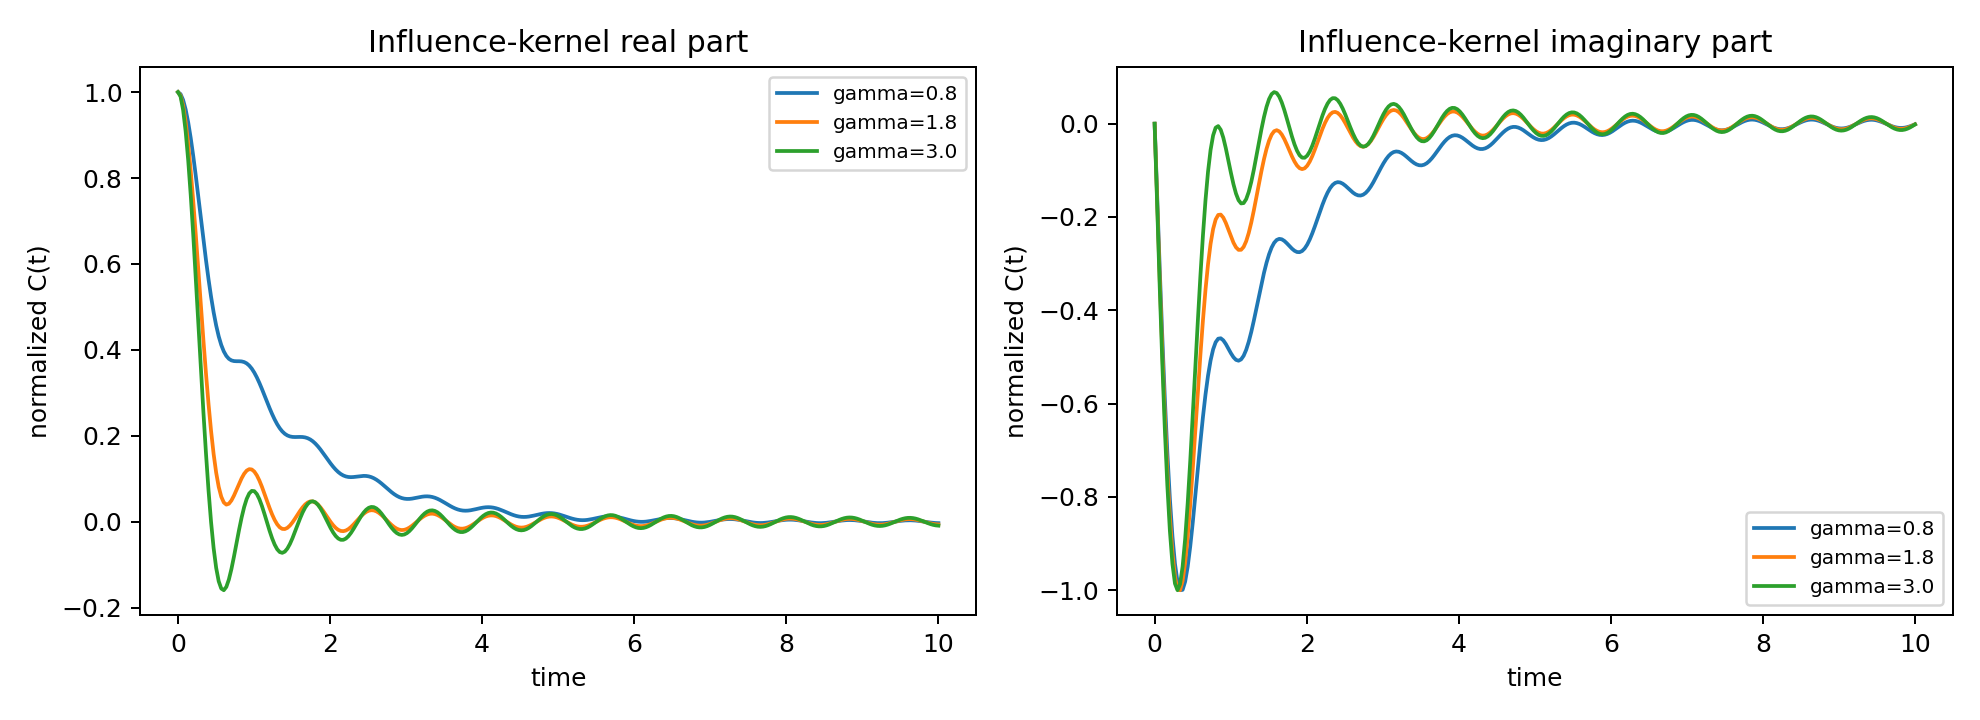
\includegraphics[width=0.32\linewidth]{path_integral_memory_kernel.png}
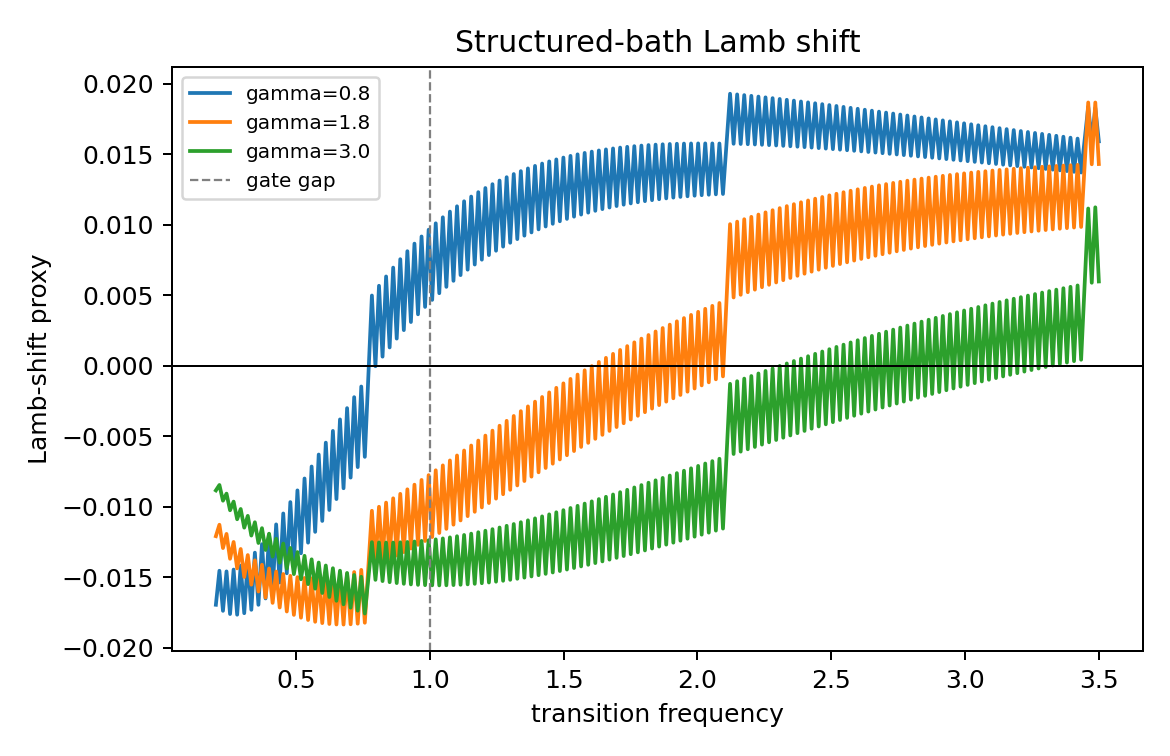
\includegraphics[width=0.32\linewidth]{structured_bath_lamb_shift.png}
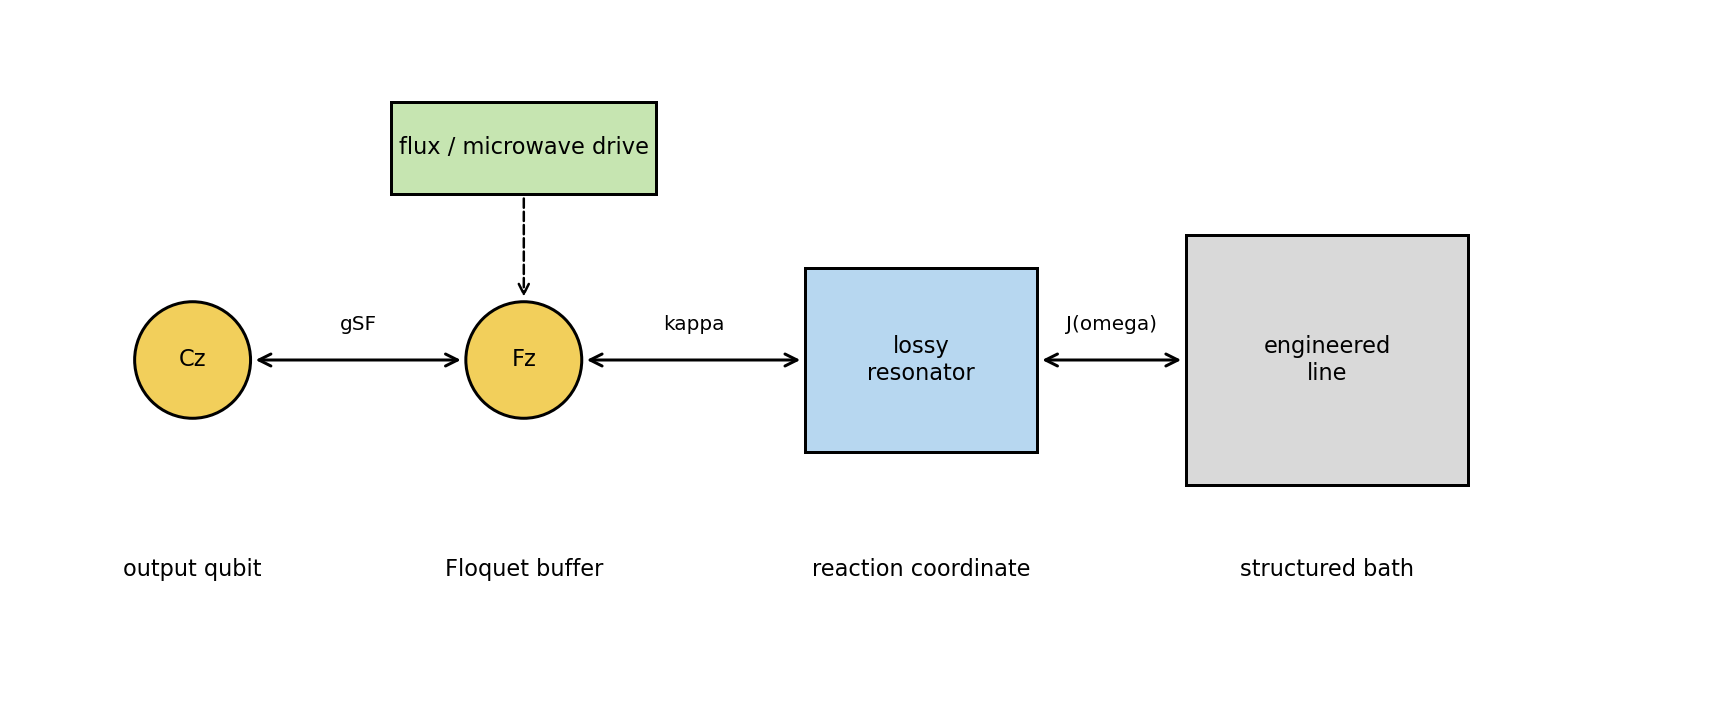
\includegraphics[width=0.32\linewidth]{qed_buffer_implementation.png}
\caption{Supporting theory and implementation figures. Left:
path-integral influence-memory kernel for different bath cutoffs.
Middle: structured-bath Lamb-shift proxy showing drive/bath-induced
detuning risk near the gate gap. Right: practical circuit-QED
implementation route for the output buffer and engineered reservoir.}
\label{fig:path-lamb-qed}
\end{figure}

\begin{figure}[H]\centering
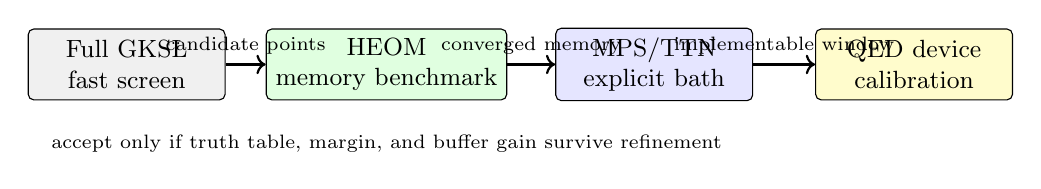
\begin{tikzpicture}[
  block/.style={rectangle, draw, rounded corners=2pt, align=center,
                minimum width=25mm, minimum height=9mm, font=\small},
  arrow/.style={->, thick}
]
\node[block, fill=gray!12] (gksl) at (0,0) {Full GKSL\\fast screen};
\node[block, fill=green!12] (heom) at (3.3,0) {HEOM\\memory benchmark};
\node[block, fill=blue!10] (mps) at (6.7,0) {MPS/TTN\\explicit bath};
\node[block, fill=yellow!20] (exp) at (10.0,0) {QED device\\calibration};
\draw[arrow] (gksl) -- (heom) node[midway,above,font=\scriptsize]{candidate points};
\draw[arrow] (heom) -- (mps) node[midway,above,font=\scriptsize]{converged memory};
\draw[arrow] (mps) -- (exp) node[midway,above,font=\scriptsize]{implementable window};
\node[font=\scriptsize, align=center] at (3.3,-1.0)
{accept only if truth table, margin, and buffer gain survive refinement};
\end{tikzpicture}
\caption{Validation pipeline used by the project: GKSL screens, HEOM
checks structured-bath memory, MPS/TTN checks explicit-reservoir scaling,
and the surviving window defines the practical QED implementation target.}
\label{fig:validation-pipeline}
\end{figure}

\subsection{Level 3: chain mapping with MPS or TTN}
For the full structured-bath gate, the scalable route is to map each
reservoir to a one-dimensional chain,
\begin{equation}
H_{B_\alpha}+H_{SB_\alpha}
\longrightarrow
\sum_{j=0}^{N_\alpha-1}\omega_{\alpha j}a_{\alpha j}^{\dagger}a_{\alpha j}
 +
\sum_{j=0}^{N_\alpha-2}t_{\alpha j}
(a_{\alpha j}^{\dagger}a_{\alpha,j+1}+\mathrm{h.c.})
 + V_{\alpha}(a_{\alpha0}+a_{\alpha0}^{\dagger}).
\label{eq:mps-chain-map}
\end{equation}
A one-branch direct benchmark is naturally an MPS if the bath chain is
ordered after the gate degrees of freedom.  For the full three-reservoir
machine, both direct and buffered geometries are naturally factor-tree
TTNs: the three-body interaction sits at the root, and the reference,
input, and output bath chains form separate branches.  The buffer only
subdivides the output branch.  This avoids forcing several independent
bath correlations through one artificial MPS bond, as quantified in
Section~\ref{sec:tn-graph}.

\begin{center}
\small
\begin{tabularx}{\textwidth}{@{}l X X@{}}
\toprule
Backend & What it proves & Required convergence test \\
\midrule
Full GKSL &
Truth table and fast robustness map in the weak-memory limit. &
Time step, Floquet period resolution, trace preservation, positivity,
and agreement with reset equations when buffers are removed. \\
HEOM &
Structured-bath memory benchmark for selected branches and selected
full-gate points. &
Hierarchy tier $N_{\mathrm{tier}}$, expansion order $K$,
Matsubara/Padé cutoff, and trace-norm convergence of $\rho_{\mathbf0}$. \\
MPS chain &
Full many-body structured-bath evolution with explicit reservoirs. &
Chain length $N_\alpha$, bosonic cutoff $d$, bond dimension $\chi$,
TDVP/Trotter time step, and recurrence-reflection time. \\
TTN chain &
Same physics as MPS, but with branch geometry matched to the gate. &
Branch bond dimensions, root tensor dimension, local truncation errors,
and comparison to MPS on small chains. \\
\bottomrule
\end{tabularx}
\end{center}

The gate is accepted only if all three statements hold: (i) the direct
and buffered models reproduce the intended Boolean truth table; (ii) the
buffered margin or distinguishability is positive after convergence; and
(iii) the sign of the buffer advantage does not flip when moving from
GKSL to HEOM and then to the MPS/TTN structured-bath simulation.

\section{Tensor networks and graph geometry}
\label{sec:tn-graph}

The earlier single-branch calculation asks how large an MPS must be once
an ordering has already been chosen.  The full gate introduces a prior
question: \emph{which tensor-network graph should be used?}  This is not
cosmetic.  The machine has three reservoir branches joined by one
three-body interaction, so flattening it into a line can force otherwise
independent branch correlations through the same virtual bond
\cite{Schollwock2011,Orus2014}.  This
section derives that graph cost and measures it on exact evolved states.

\subsection{Hamiltonian hypergraph, primal graph, and factor tree}
Let the physical vertices be
\begin{equation}
 V=\{C_0,C_1,C_z,F,B_{\alpha j}:\alpha\in\{0,1,z\}\},
 \label{eq:tn-vertices}
\end{equation}
where $F$ is omitted for direct contact.  Pair interactions give ordinary
edges, but the gate term is the hyperedge
\begin{equation}
 e_3=\{C_0,C_1,C_z\},\qquad
 H_3=g_3\left(\sigma_+^{(0)}\sigma_-^{(1)}\sigma_-^{(z)}
 +\sigma_-^{(0)}\sigma_+^{(1)}\sigma_+^{(z)}\right).
 \label{eq:tn-three-body-hyperedge}
\end{equation}
There are two standard graph representations.  The \emph{primal graph}
replaces $e_3$ by the triangle
$(C_0,C_1),(C_0,C_z),(C_1,C_z)$.  It contains one cycle and has treewidth
$2$.  The \emph{incidence} or factor graph instead introduces one
nonphysical factor vertex $U_3$ and connects it separately to
$C_0$, $C_1$, and $C_z$.  After each reservoir is chain mapped,
this incidence graph is a tree and therefore has treewidth $1$.

This replacement is exact at the operator level rather than an
approximation.  Equation~\eqref{eq:tn-three-body-hyperedge} is a sum of
two product operators, so the central Hamiltonian factor has canonical
polyadic operator rank $2$.  The passive buffer merely subdivides the
output edge as $C_z-F-B_{z1}$.  The Floquet term
\begin{equation}
 H_D(t)=A\cos(\Omega t)\sigma_x^{(F)}
 \label{eq:tn-local-floquet-factor}
\end{equation}
is local on $F$; consequently it adds no spatial graph edge and cannot
change treewidth.  It can still change the numerical bond dimensions by
creating more entanglement during time evolution.

\begin{figure}[H]\centering
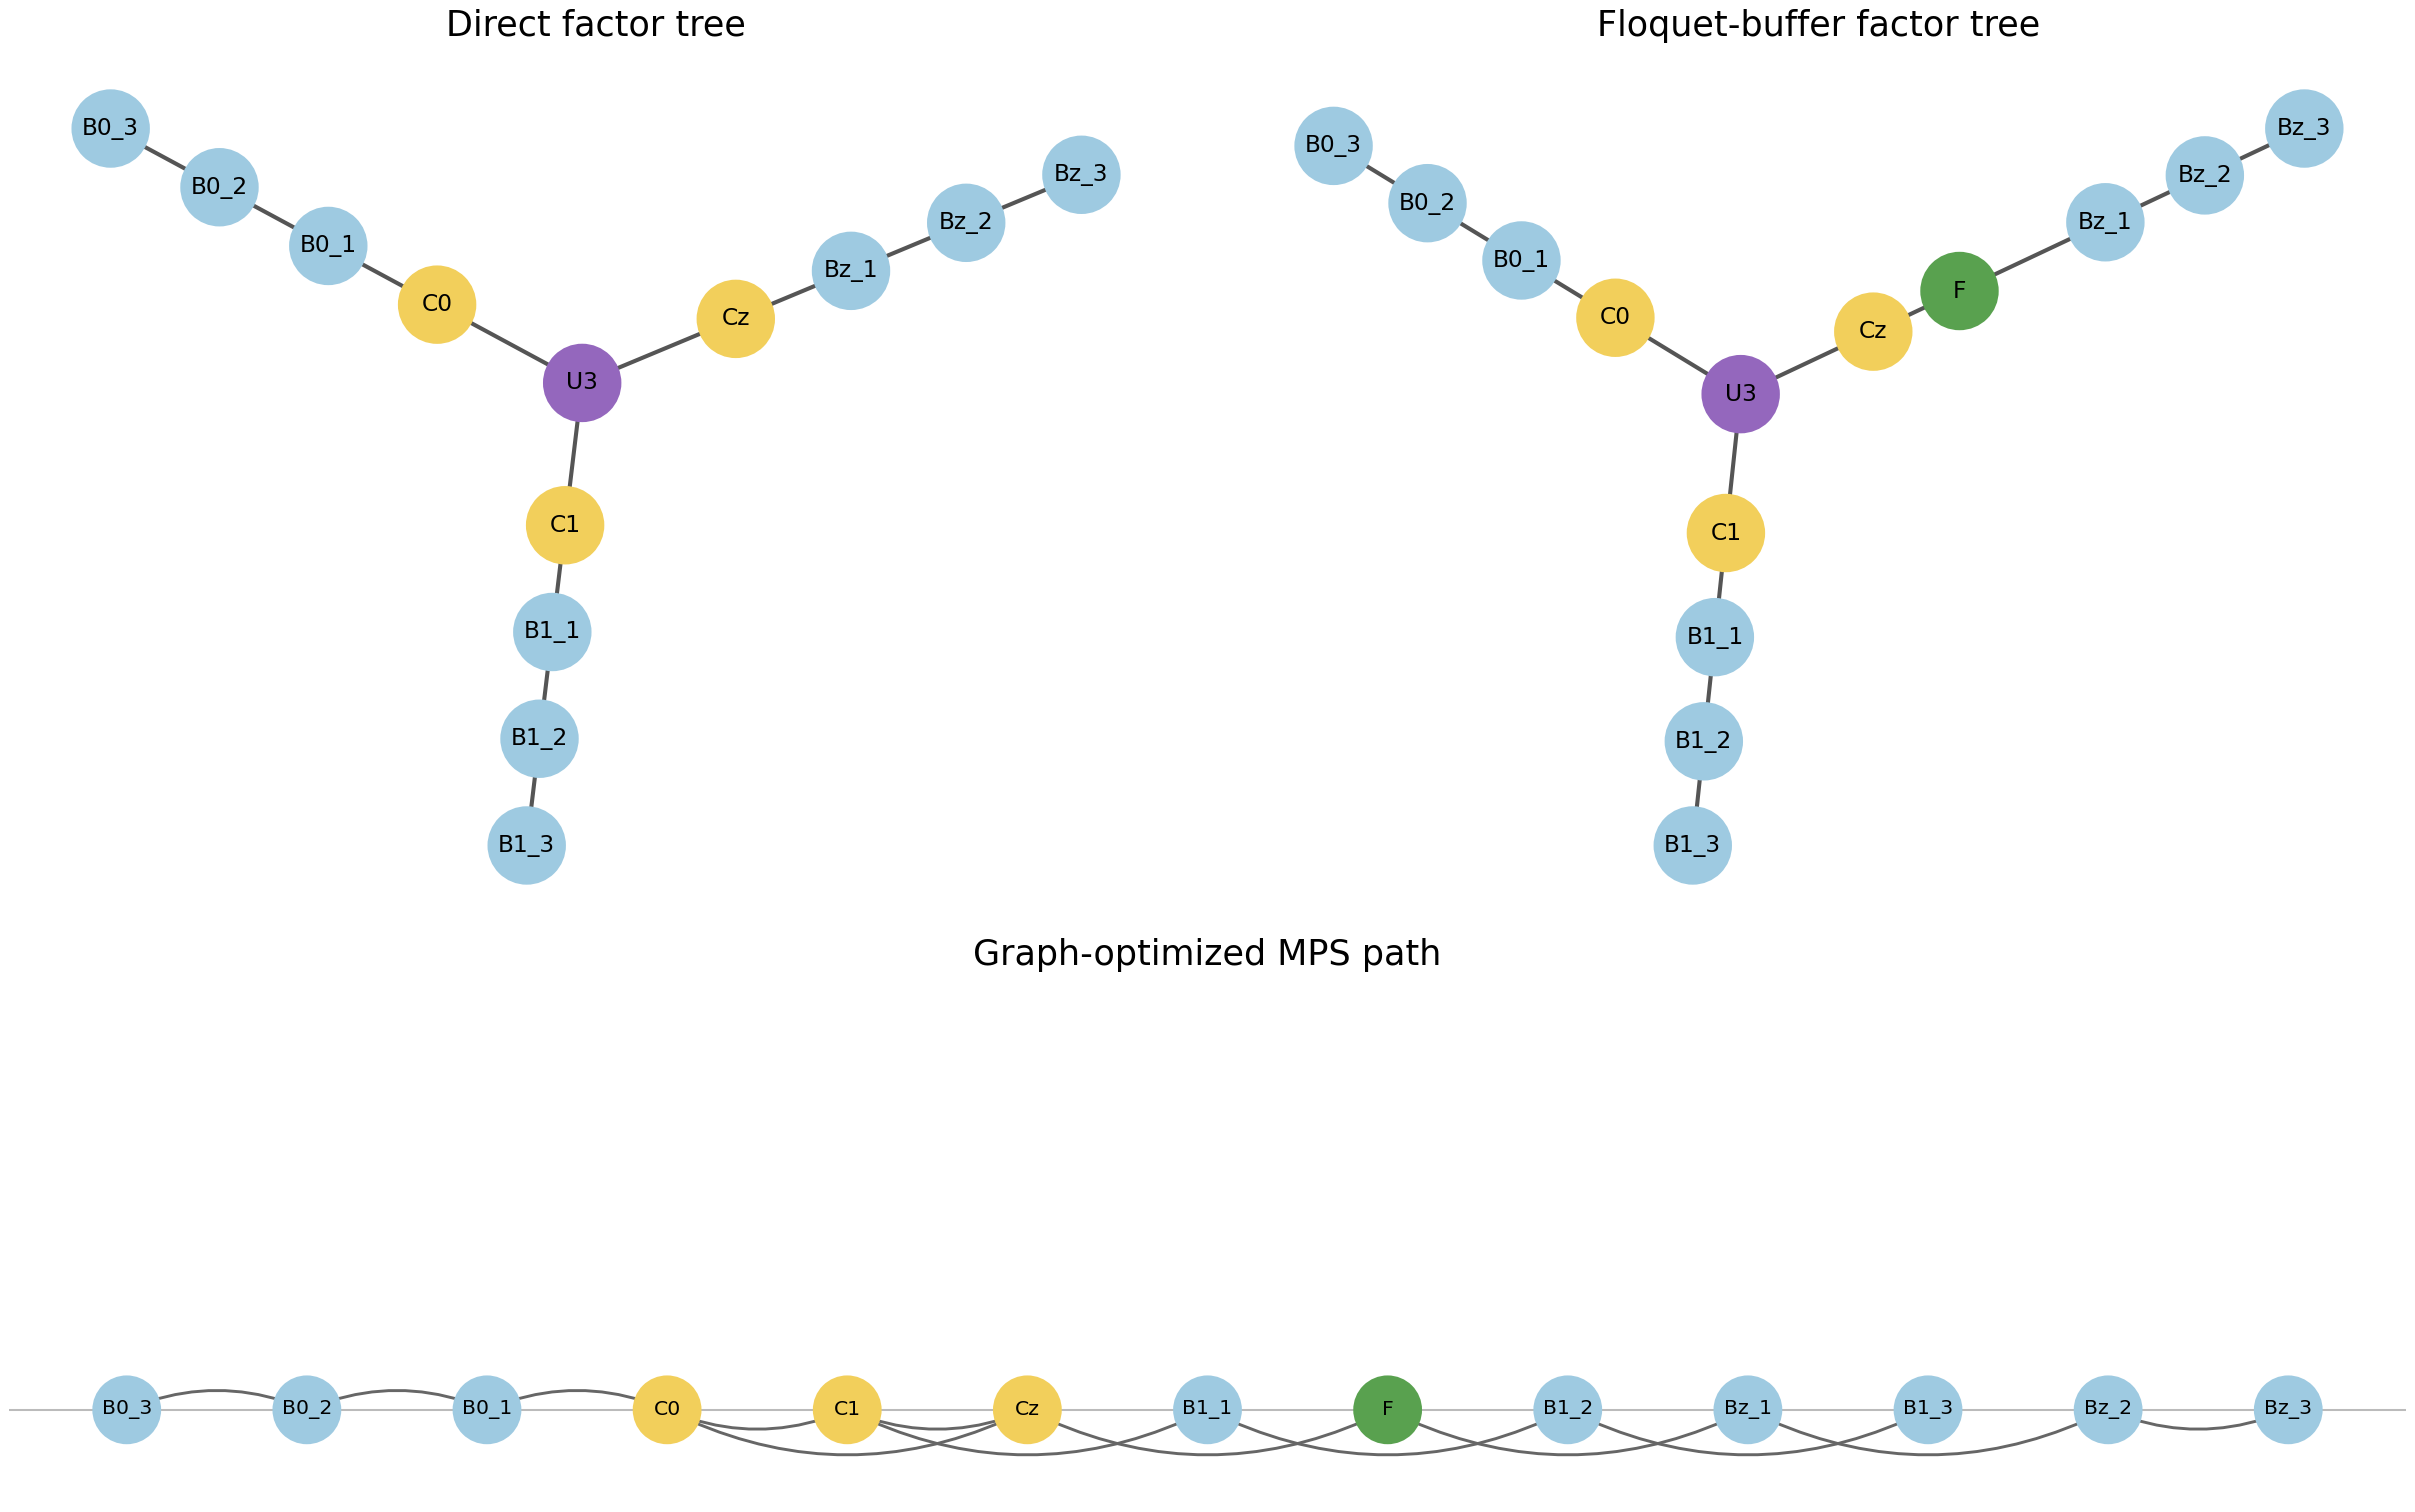
\includegraphics[width=0.99\linewidth]{tensor_network_graph_topologies.png}
\caption{Tensor-network geometry of the three-reservoir machine.  The
purple $U_3$ tensor represents the three-body interaction.  Direct and
Floquet-buffered incidence graphs are trees; the buffer subdivides one
branch without creating a cycle.  The right panel shows a graph-optimized
MPS ordering, where curved interaction edges reveal the price of forcing
the branched graph onto one path.}
\label{fig:tn-graph-topologies}
\end{figure}

\subsection{Deriving the MPS ordering cost}
An MPS first chooses a bijection
$\pi:V\rightarrow\{1,\ldots,n\}$.  Its $k$th bond separates the prefix
\begin{equation}
 S_k^\pi=\{v:\pi(v)\leq k\}
 \label{eq:tn-prefix-set}
\end{equation}
from its complement.  For an interaction graph $G=(V,E)$, define the
edge boundary and ordering cutwidth
\begin{align}
 \delta_G(S)&=\{(u,v)\in E:u\in S,\ v\notin S\},\\
 c(\pi)&=\max_{1\leq k<n}|\delta_G(S_k^\pi)|.
 \label{eq:tn-cutwidth}
\end{align}
The bandwidth
\begin{equation}
 b(\pi)=\max_{(u,v)\in E}|\pi(u)-\pi(v)|
 \label{eq:tn-bandwidth}
\end{equation}
measures the longest interaction in the linear layout.  Cutwidth controls
how many interactions can create entanglement across one MPS bond, while
bandwidth controls how many swap gates or long-range MPO channels are
needed by a nearest-neighbour implementation.  They are graph proxies,
not substitutes for measuring the evolved state.

For a pure state, the Schmidt decomposition at cut $k$ is
\begin{equation}
 |\psi\rangle=\sum_{r=1}^{R_k}s_{k r}
 |L_{k r}\rangle|R_{k r}\rangle,
 \qquad \sum_r s_{k r}^2=1.
 \label{eq:tn-schmidt}
\end{equation}
Given an allowed discarded weight $\varepsilon$, the minimal numerical
bond dimension is
\begin{equation}
 \chi_k^\star(\varepsilon)
 =\min\left\{q:\sum_{r>q}s_{k r}^2\leq\varepsilon\right\},
 \qquad
 \chi_{\rm MPS}^\star=\max_k\chi_k^\star .
 \label{eq:tn-minimal-chi}
\end{equation}
The bond entropy
\begin{equation}
 S_k=-\sum_r s_{k r}^2\log_2 s_{k r}^2
 \label{eq:tn-bond-entropy}
\end{equation}
obeys $S_k\leq\log_2\chi_k$.  For local evolution, entanglement can be
generated across the cut only by terms in $\delta_G(S_k)$; schematically,
\begin{equation}
 \left|\frac{\mathrm d S_k}{\mathrm dt}\right|
 \lesssim c_{\mathrm{ent}}\sum_{e\in\delta_G(S_k)}\|h_e\|\log d_e .
 \label{eq:tn-entanglement-rate-bound}
\end{equation}
Thus minimizing $c(\pi)$ is a principled ordering heuristic, although
destructive interference and unequal couplings mean that the Schmidt
spectrum remains the final numerical test.

If the MPS bond dimensions are $\chi_0=\chi_n=1$ and
$\chi_1,\ldots,\chi_{n-1}$, its raw tensor-entry count is
\begin{equation}
 P_{\rm MPS}=\sum_{k=1}^{n}d_k\chi_{k-1}\chi_k .
 \label{eq:tn-mps-parameters}
\end{equation}
This count is representation dependent and includes gauge redundancy,
but it is a useful memory and contraction-cost proxy when comparing two
topologies for the same state.

\subsection{Why a topology-matched TTN is different}
For the factor-tree topology $T$, removing an edge $e$ partitions the
physical leaves into $A_e$ and $\bar A_e$.  The smallest exact TTN bond
on that edge is the Schmidt rank of this bipartition; with truncation,
\begin{equation}
 \chi_e^\star(\varepsilon)
 =\min\left\{q:\sum_{r>q}s_{e r}^2\leq\varepsilon\right\}.
 \label{eq:tn-ttn-chi}
\end{equation}
Every reservoir branch is disconnected from the rest by one factor-tree
edge, so its graph boundary is one independently of chain length.  A
linear MPS cannot place all three branches on opposite sides of the
central interaction simultaneously.  The TTN therefore trades the path
bottleneck for a higher-degree root tensor.  Its raw entry count is
\begin{equation}
 P_{\rm TTN}=\sum_{v\in T}d_v\prod_{e\ni v}\chi_e,
 \qquad d_{U_3}=1,\qquad d_v=2\text{ for a spin site}.
 \label{eq:tn-ttn-parameters}
\end{equation}
The root product in Eq.~\eqref{eq:tn-ttn-parameters} is the principal TTN
cost.  A TTN is advantageous only if the reduction of branch bond
dimensions compensates for this product; the exact-state experiment
below checks that condition directly.

\subsection{Exact graph-state experiment and Quimb MPS compression}
The reproducible code in
\texttt{Scripts/tensor\_network\_graph\_analysis/} performs two tests.
First, it builds direct, passive-buffer, and Floquet-buffer graphs for
$L=1,\ldots,10$, evaluates an interleaved ordering, and searches
deterministically over breadth-first, depth-first, reverse
Cuthill--McKee, reversed, and local-swap orderings.  At $L=10$ all three
architectures have primal-treewidth upper bound $2$ and factor-treewidth
$1$.  The interleaved MPS has cutwidth $4$, the optimized MPS has
cutwidth $3$, and the factor-tree TTN has separator width $1$.  These
widths remain constant with $L$ because extending a branch adds vertices
but no new junction.

Second, a state-level benchmark uses the finite spin Hamiltonian
\begin{align}
 H_{\rm geom}(t)
 &=\frac12\sum_v\omega_v\sigma_z^{(v)}+H_3
 +\sum_{(u,v)\in E_2}J_{uv}\sigma_x^{(u)}\sigma_x^{(v)}
 +\mathbf{1}_{\rm Floquet}A\cos(\Omega t)\sigma_x^{(F)} .
 \label{eq:tn-geometry-hamiltonian}
\end{align}
The chosen dimensionless values are
$(\omega_0,\omega_1,\omega_z,\omega_F)=(2,1,1,1)$,
$\omega_{B_j}=0.82+0.04j$, $g_3=0.18$, contact coupling $0.14$,
$C_z$--$F$ coupling $0.12$,
$J_j=0.11/[1+0.15(j-1)]$, $A=0.45$, and $\Omega=1.3$.
Sparse exact propagation uses $24$ midpoint steps over $0\leq t\leq4$.
The largest calculations contain $15$ physical spins for direct contact
and $16$ for buffered contact.  Schmidt spectra are sampled every four
steps using discarded-weight tolerance $\varepsilon=10^{-10}$.  The
final state is also factorized and compressed as an MPS using Quimb
\cite{Gray2018}.

\begin{table}[H]\centering\small
\caption{Maximum tolerance-controlled tensor requirements for exactly
evolved states over the $L=4$ time
window.  $P$ is the maximum raw tensor-entry count.  $F_{\chi=8}$ is the
final-state fidelity after graph-ordered Quimb MPS compression.}
\label{tab:tn-exact-results}
\begin{tabular}{@{}l r r r r r r@{}}
\toprule
Architecture & $\chi_{\rm int}$ & $\chi_{\rm opt}$ & $\chi_{\rm TTN}$ &
$P_{\rm opt}$ & $P_{\rm TTN}$ & $F_{\chi=8}$ \\
\midrule
Direct & 61 & 23 & 10 & 4332 & 1702 & 0.9999693 \\
Passive buffer & 66 & 23 & 10 & 4650 & 1740 & 0.9999745 \\
Floquet buffer & 65 & 25 & 10 & 4986 & 1646 & 0.9999718 \\
\bottomrule
\end{tabular}
\end{table}

The ordering effect is already substantial: relative to interleaving,
graph optimization reduces the maximum required MPS bond from $61$ to
$23$ for direct contact and from $65$ to $25$ for the Floquet buffer.
The topology-matched TTN reduces the maximum to $10$.  Its raw entry
count is smaller than optimized MPS by $60.7\%$ (direct), $62.6\%$
(passive), and $67.0\%$ (Floquet).  The Floquet drive leaves all graph
widths unchanged but raises the observed optimized-MPS maximum from $23$
for the passive buffer to $25$ for the driven buffer.  Geometry and
dynamics are therefore distinct sources of cost.

\begin{figure}[H]\centering
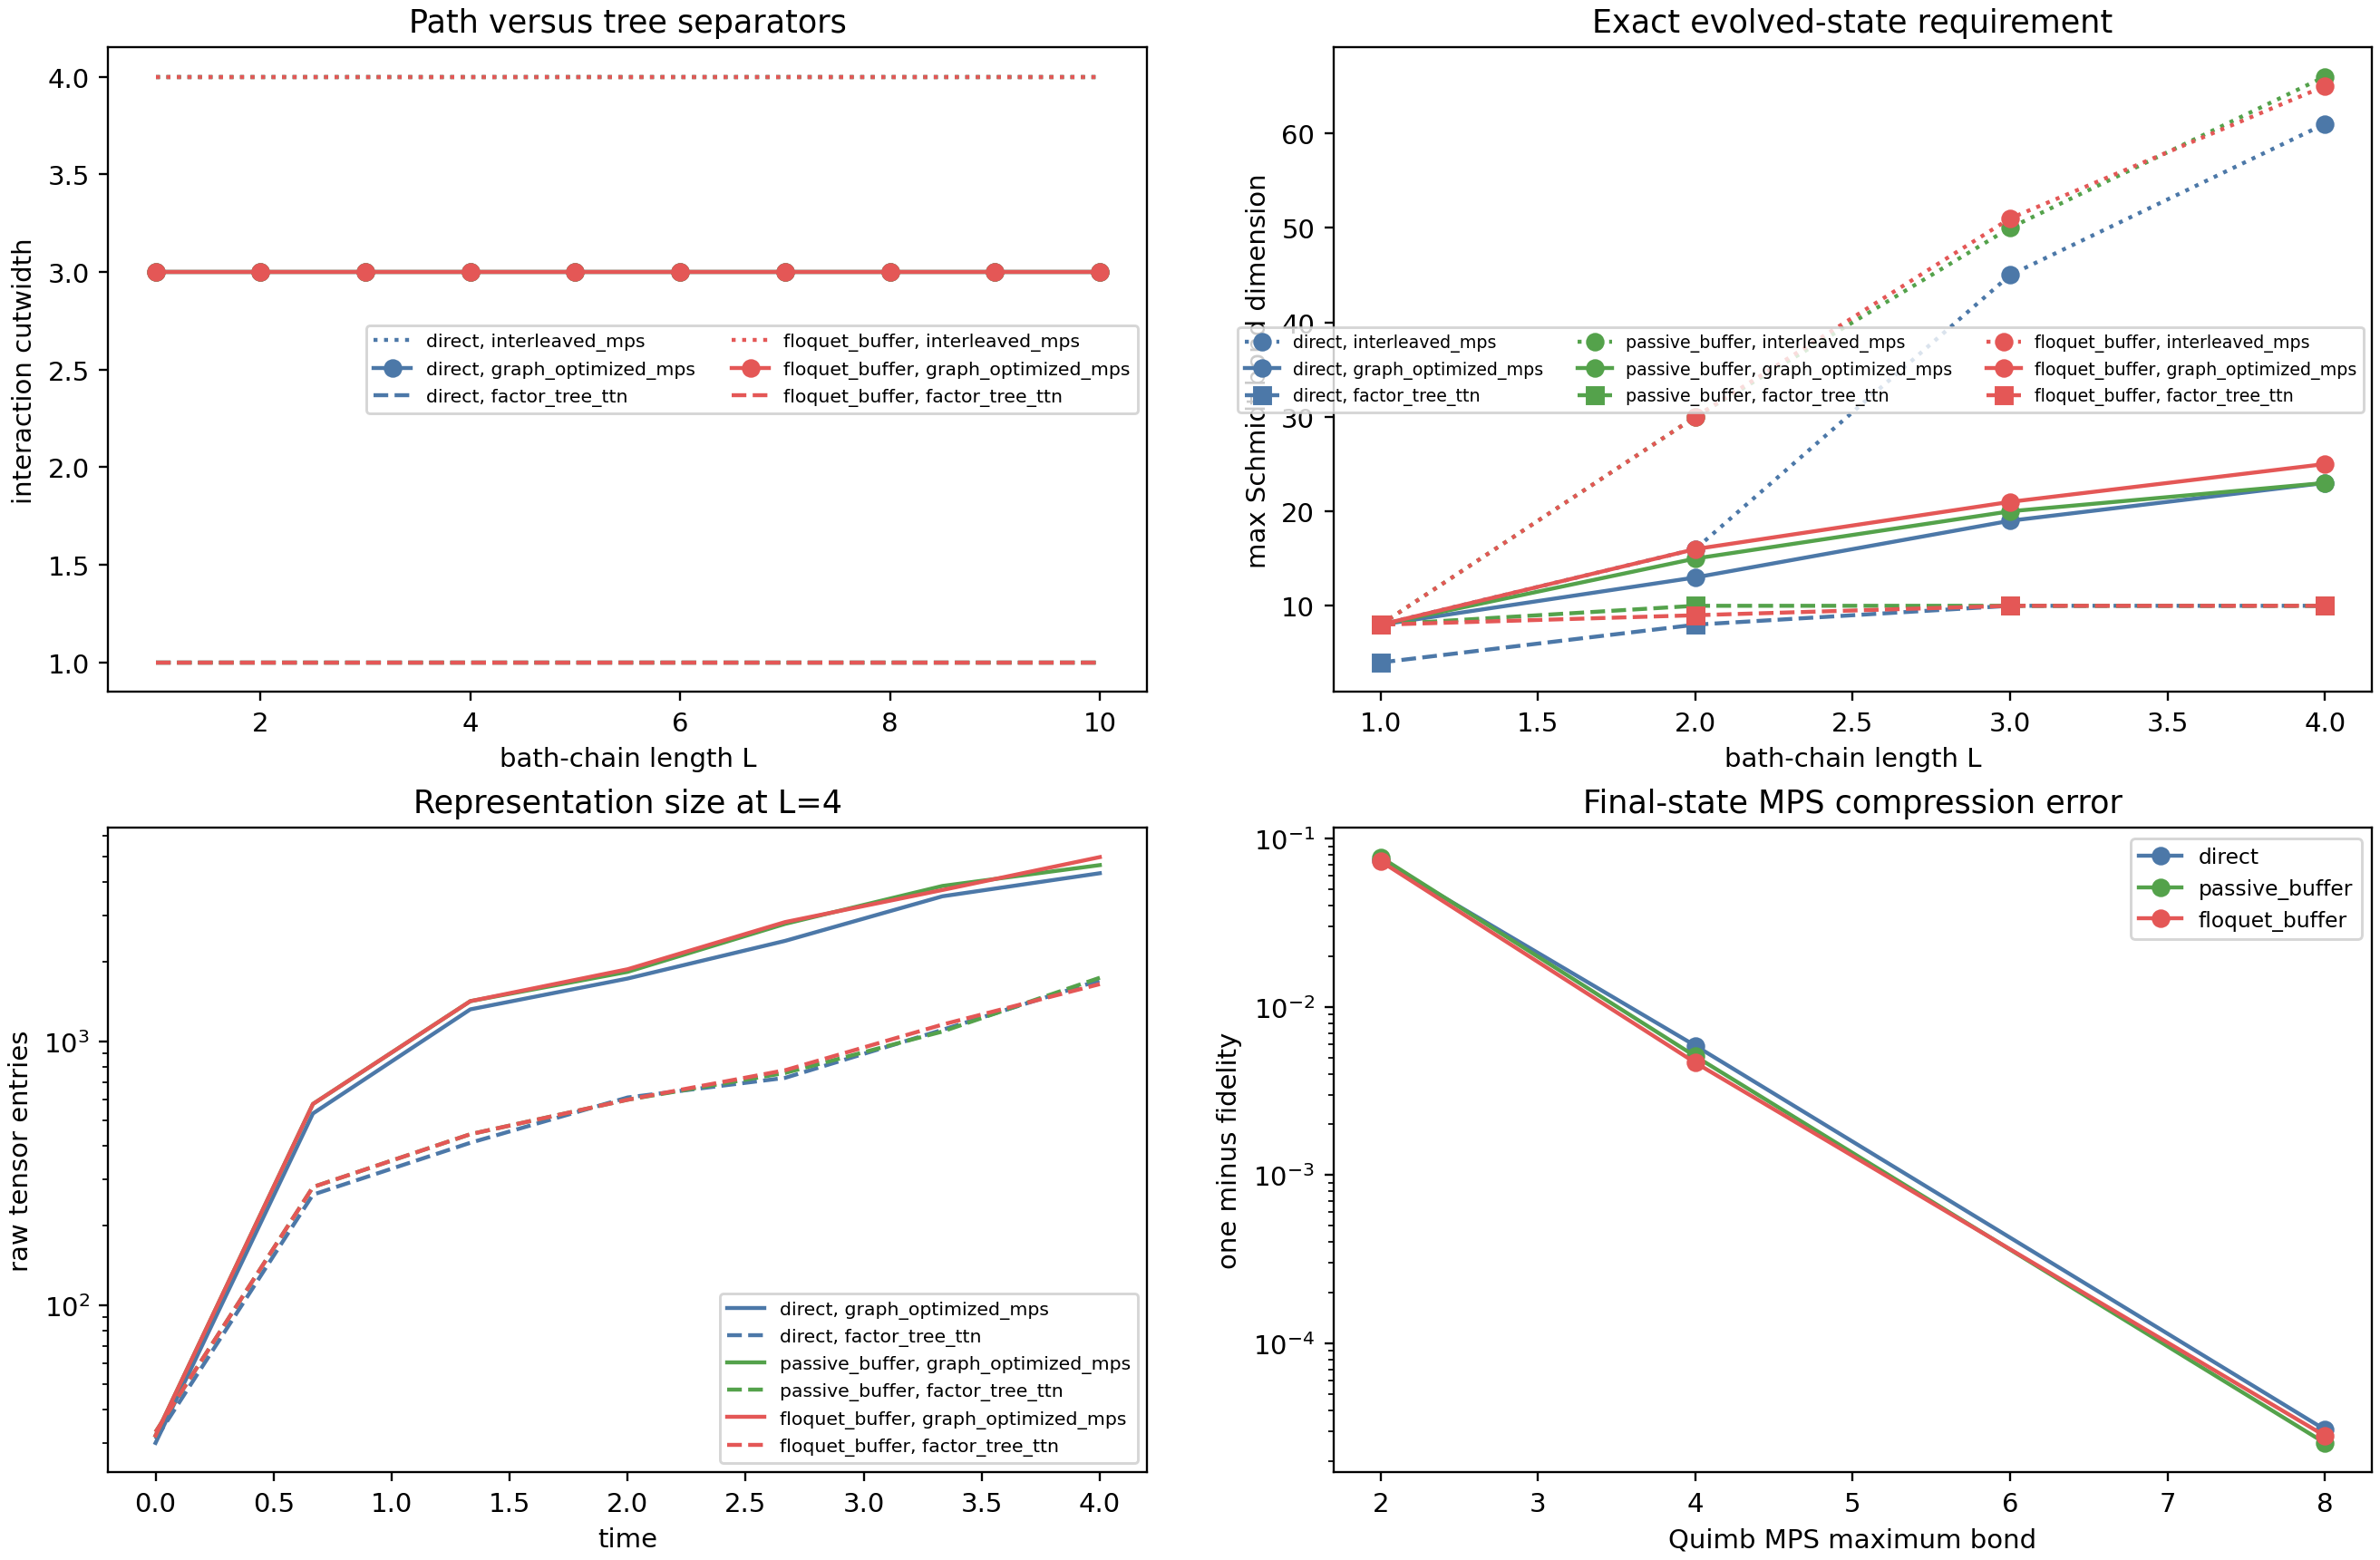
\includegraphics[width=0.99\linewidth]{mps_ttn_graph_scaling.png}
\caption{Graph and exact-state tensor-network benchmark.  Top left:
MPS cutwidth depends on ordering, while every factor-tree TTN edge is a
one-edge separator.  Top right: maximum required Schmidt bond over the
exact time window.  Bottom left: raw tensor entries at $L=4$; dashed TTN
curves remain below optimized MPS curves.  Bottom right: graph-ordered
Quimb MPS compression error, showing that $\chi=8$ already retains more
than $0.9999$ fidelity despite the stricter $10^{-10}$ discarded-weight
ranks reported in the table.}
\label{fig:mps-ttn-graph-scaling}
\end{figure}

\subsection{What this establishes and what remains}
The calculation establishes four points.  First, the natural mathematical
object is a hypergraph/factor graph, not a single bath chain.  Second,
site ordering is an algorithmic variable: a poor ordering can cost more
than adding the physical buffer.  Third, the factor-tree TTN is the
lowest-rank exact representation tested for the full three-branch
geometry.  Fourth, an optimized MPS remains an excellent validation
backend because a modest $\chi=8$ gives final-state fidelity above
$0.9999$ in all three cases.

This is deliberately not presented as a converged thermodynamic-gate
simulation.  Approximations (A12)--(A14) replace bosonic modes by spins,
use a pure product preparation, stop before long-chain steady-state
physics, and factorize exact small-system states instead of evolving the
tensor network variationally.  The next tensor-network experiment should
therefore use orthogonal-polynomial chain coefficients, thermofield
purification of each thermal bath, two-site TDVP or TEBD, and independent
convergence in $(L,d,\chi,\Delta t)$.  The graph result gives a concrete
backend decision for that calculation: use MPS for single branches and
cross-checks, but use the factor-tree TTN as the primary full-gate
geometry.

\section{Architecture decision and CMOS--inverter correspondence}
\label{sec:architecture-decision}

\subsection{Three realizable bath-contact architectures}
The numerical word ``buffered'' contains two different physical ideas:
inserting an intermediate subsystem and driving that subsystem.  They
must be separated before asking whether the Floquet architecture is
actually better.  For one output operator $S$ and bath operator $B$, the
three Hamiltonian topologies are
\begin{align}
 H_{\rm direct}
 &=H_{\rm M}+H_B+g_{MB}S\otimes B,
 \label{eq:architecture-direct}\\
 H_{\rm passive}
 &=H_{\rm M}+H_F+g_{MF}S\otimes F+H_B+g_{FB}F\otimes B,
 \label{eq:architecture-passive}\\
 H_{\rm Floquet}(t)
 &=H_{\rm passive}+A\cos(\Omega t+\phi)F_x .
 \label{eq:architecture-floquet}
\end{align}
Here M denotes the integrated autonomous thermal machine.  The direct and
passive Hamiltonians are time independent and therefore strictly
autonomous once the thermal reservoirs are connected.  The passive
subsystem $F$ may be a reaction-coordinate resonator, auxiliary qubit, or
impedance filter.  The Floquet device is a hybrid thermal machine: its
heat currents still perform the logic, but an external phase reference
and work source continuously modulate $F$.

\begin{figure}[H]\centering
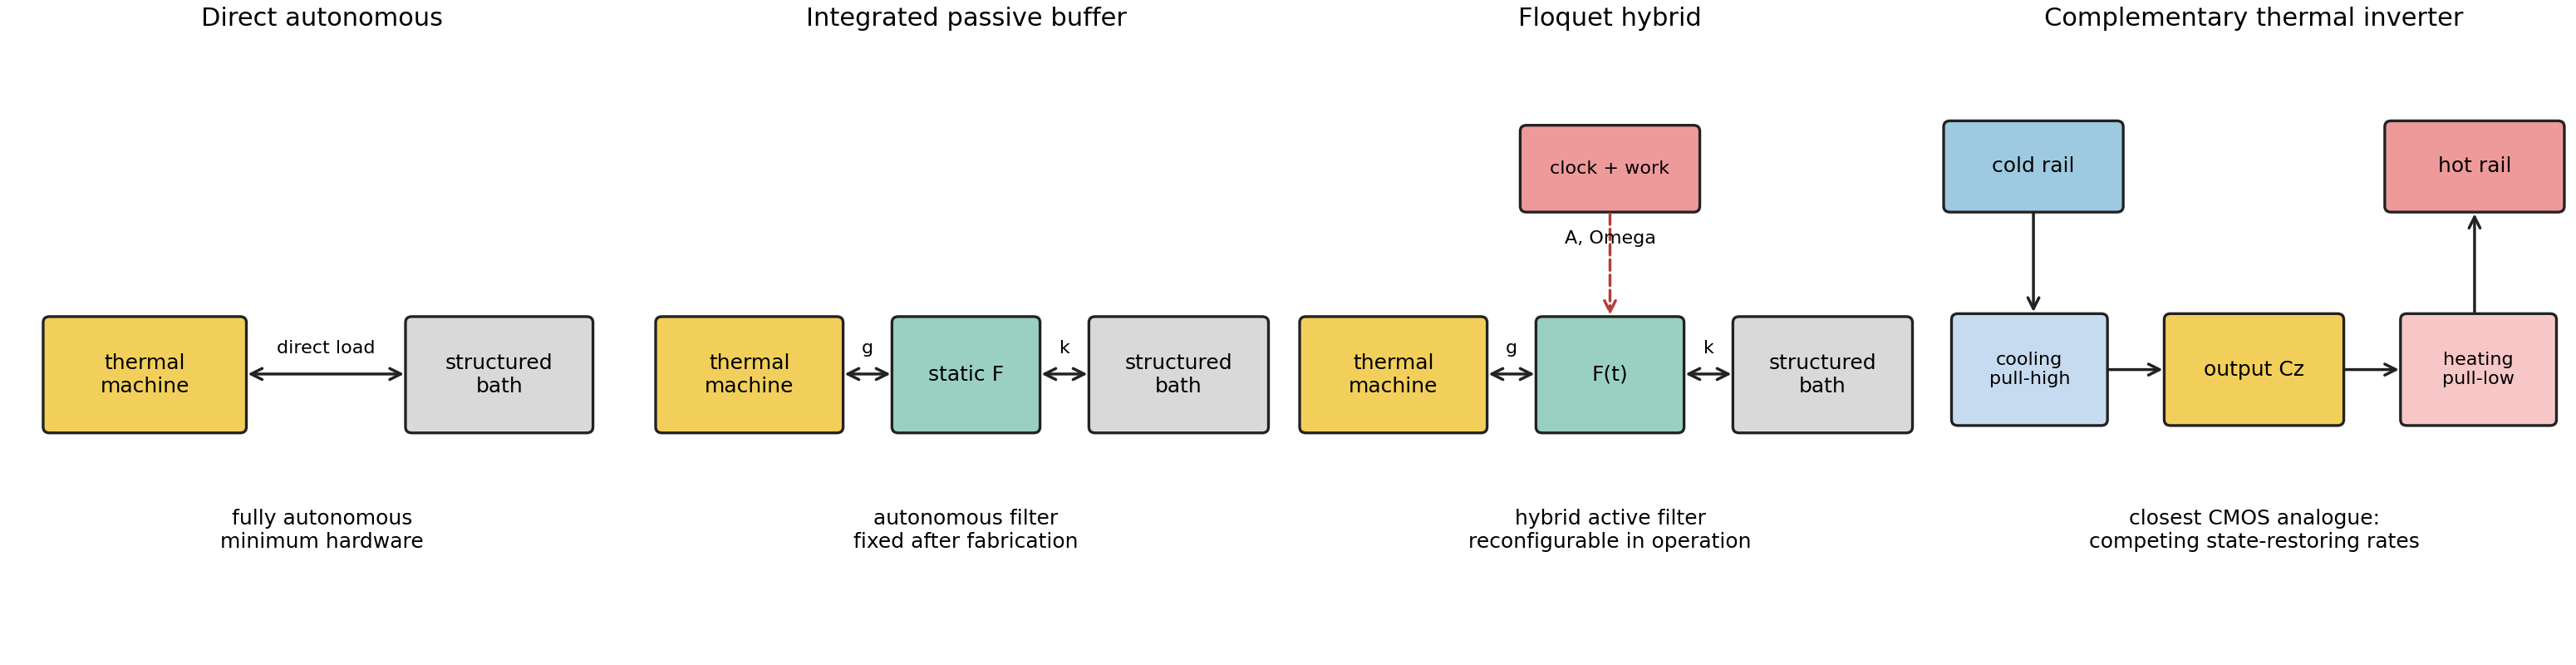
\includegraphics[width=0.99\linewidth]{thermal_architecture_schematic.png}
\caption{Four architecture classes.  Direct contact minimizes hardware;
the static integrated buffer preserves autonomy while filtering the bath;
the Floquet hybrid adds in-operation spectral control; and a genuinely
CMOS-like thermal inverter requires complementary pull-high and pull-low
dissipative channels rather than one buffer alone.}
\label{fig:thermal-architecture-schematic}
\end{figure}

For matched bath and coupling parameters, define the exact decomposition
\begin{equation}
 \underbrace{D_F(A)-D_{\rm direct}}_{\text{total buffered gain}}
 =\underbrace{D_F(0)-D_{\rm direct}}_{\text{passive isolation}}
 +\underbrace{D_F(A)-D_F(0)}_{\text{drive-specific Floquet gain}}.
 \label{eq:buffer-gain-decomposition}
\end{equation}
At the best-gain HEOM bath point
$(g_{SF},\lambda,\gamma_c)=(0.04,0.075,0.8)$, direct contact gives
$D_{\rm direct}=0.353784$, the static integrated buffer gives
$D_F(0)=0.966563$, and the best driven setting gives
$D_F(0.55)=0.977156$.  Therefore
\begin{equation}
 \Delta D_{\rm total}=0.623372
 =0.612779+0.010593 .
 \label{eq:best-gain-decomposition}
\end{equation}
Approximately $98.3\%$ of the total improvement at this point comes from
inserting the intermediate subsystem; only $1.7\%$ is the incremental
effect of driving it.  The driven increment costs
$W_{\rm abs}=0.559420$ in the dimensionless work-throughput convention of
Eq.~\eqref{eq:work-accounting}.

This single point does not make the drive irrelevant.  Repeating the
matched comparison for all $243$ driven HEOM points gives
\begin{equation}
 D_F(A)-D_F(0)>0\quad\text{for }243/243\text{ points},
 \label{eq:all-driven-improve}
\end{equation}
with median increment $0.020150$, empirical $5$--$95\%$ interval
$[0.002450,0.164534]$, and maximum increment $0.263747$.  Larger drive
amplitudes have larger median increments, and the largest gains occur
when the static buffer is less well matched.  Thus periodic control is
most defensible as a \emph{tunable rescue and calibration layer}, not as
the sole origin of isolation.

\begin{figure}[H]\centering
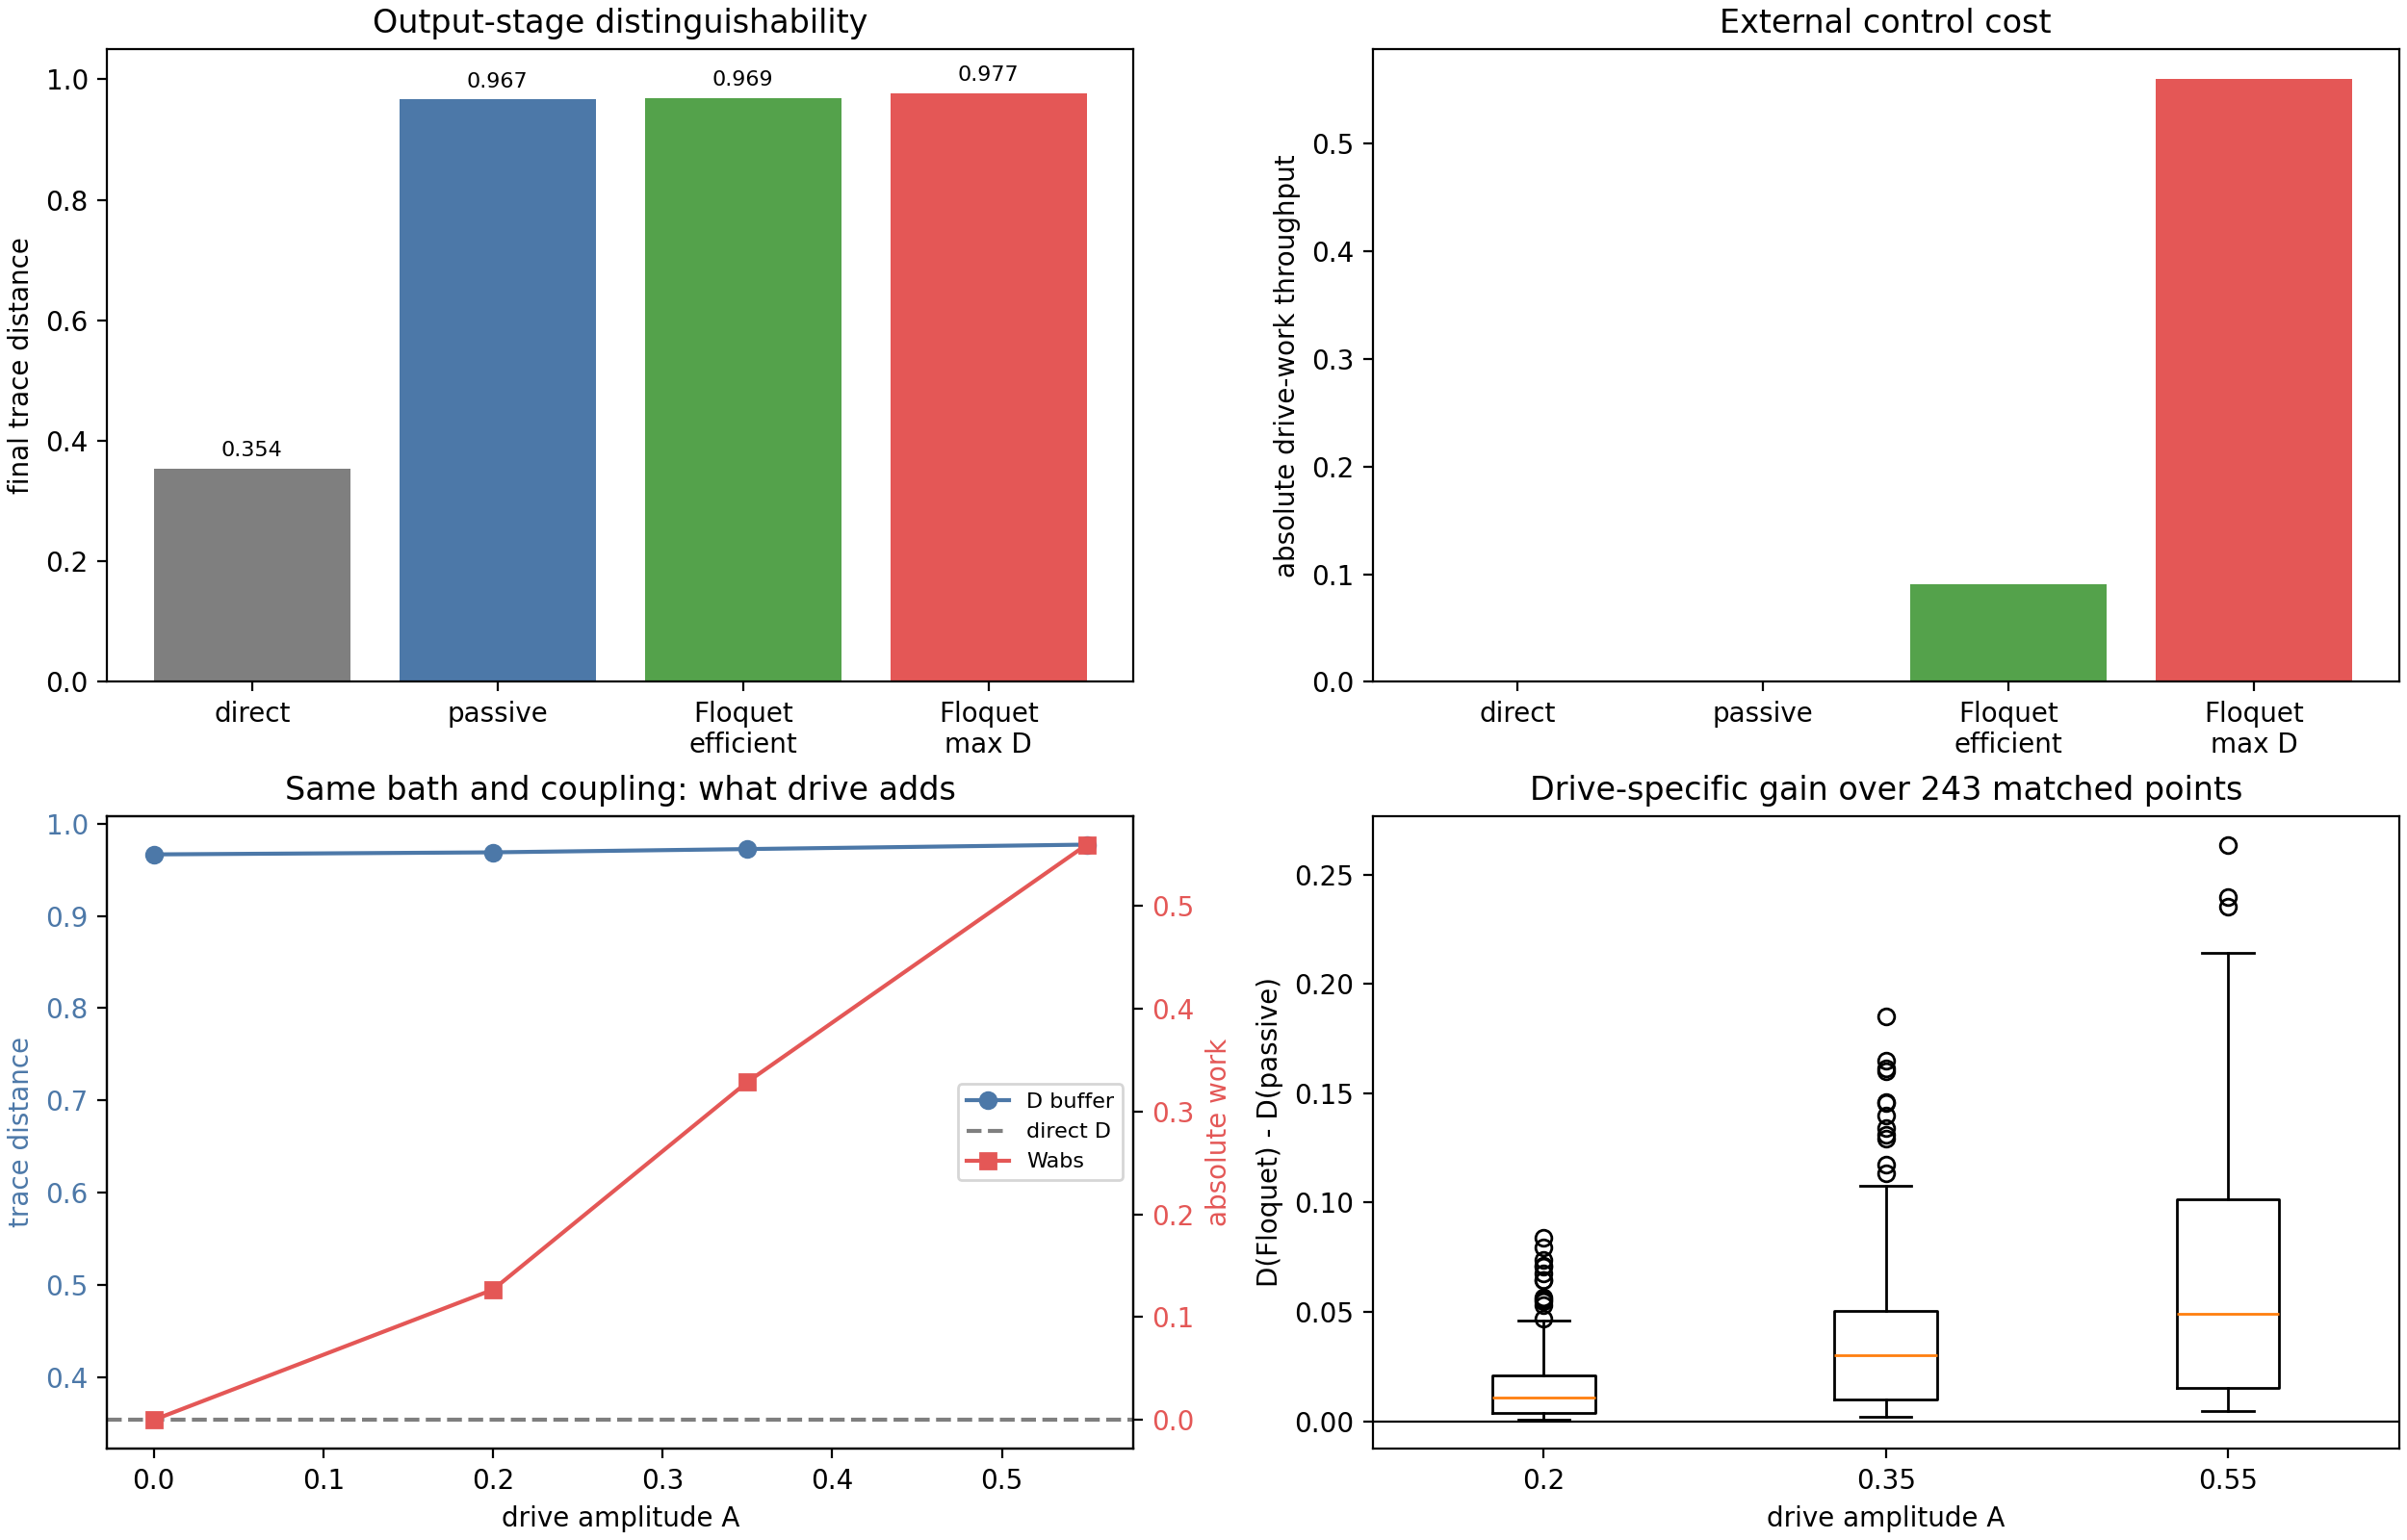
\includegraphics[width=0.96\linewidth]{architecture_performance_tradeoff.png}
\caption{Architecture-level HEOM comparison.  Top: distinguishability and
external drive throughput for direct, passive, and two driven operating
points.  Bottom left: adding drive at one fixed bath/coupling point gives
a small increase in $D$ while work grows.  Bottom right: distribution of
the drive-specific increment over all $243$ matched driven/passive pairs.}
\label{fig:architecture-performance}
\end{figure}

The earlier reduced bridge ablation found that its default undriven
spacer degraded distinguishability, whereas the broader HEOM sweep finds
strong passive-buffer performance at weak $g_{SF}$.  These results are not
mathematically contradictory: the Hamiltonians, bath descriptions, and
parameter points differ.  Their combination establishes the more useful
claim that a static buffer is \emph{not automatically} beneficial; it must
be impedance- and frequency-matched, while Floquet control expands the
set of parameters that can be repaired after fabrication.

\subsection{Is the Floquet architecture actually better?}
There is no architecture-independent yes/no answer because ``better''
requires an objective function.  A minimal decision functional is
\begin{equation}
 \mathcal C_a
 =w_D(1-D_a)+w_W W_{{\rm abs},a}
 +w_C C_{{\rm control},a}+w_H C_{{\rm hardware},a},
 \label{eq:architecture-cost}
\end{equation}
where the weights encode whether a device values logical fidelity,
external work, control electronics, or component count.  The computed
results support the following conditional decision.

\begin{table}[H]\centering\small
\caption{Architecture decision from the present simulations.  Numerical
$D$ values refer to the same selected reduced output-stage HEOM point and
are not a full-device energy comparison.}
\label{tab:architecture-decision}
\begin{tabularx}{\textwidth}{@{}l X X X@{}}
\toprule
Criterion & Direct autonomous contact & Integrated passive buffer & Floquet buffer \\
\midrule
Final $D$ at selected bath & $0.353784$ & $0.966563$ & $0.977156$ \\
External drive throughput & $0$ & $0$ & $0.559420$ at maximum-$D$ point \\
Strict autonomy & Yes & Yes & No: clock and work source required \\
Spectral isolation & None beyond bare coupling & Fixed by $H_F,g_{MF},g_{FB}$ & Sideband-tunable during operation \\
Fabrication/calibration & Lowest component count & Extra resonator/qubit and fixed matching & Extra subsystem, drive line, phase and Lamb-shift calibration \\
Best use case & Benign Markovian bath; minimum hardware & Stable structured bath known at design time & Unknown/drifting spectrum or post-fabrication retuning \\
Current evidence & Lowest work but weak $D$ in hard-memory point & Captures most of the HEOM gain & Improves every matched passive point, often modestly \\
\bottomrule
\end{tabularx}
\end{table}

Hence the \emph{integrated passive buffer is the preferred default
architecture under the present fixed-parameter evidence}: it preserves
autonomy and obtains nearly all of the best-point distinguishability.
The Floquet buffer is better when its reconfigurability has operational
value---for example compensating fabrication disorder, tracking a moving
bath resonance, widening a robust operating window, or shortening a
calibration cycle.  Direct contact remains rational when the reservoir is
already weak and Markovian, component count dominates, or any external
clock is disallowed.  The Floquet branch therefore does not dominate the
autonomous alternatives in the Pareto sense: it increases $D$ but also
increases work and control complexity.

This conclusion is intentionally limited to the reduced HEOM output
stage.  A final device-level ranking needs the full gate truth table,
steady heat currents, entropy production, reset cost, drive-line loss,
and fabrication overhead evaluated in one common model.  In particular,
$W_{\rm abs}$ is not the wall-plug power of a cryogenic microwave source.

\subsection{Deriving the CMOS comparison}
The analogy to a CMOS inverter is useful only after specifying the
transfer law.  In a symmetric long-channel square-law model, define
\begin{equation}
 I(\Delta,V_D)=k
 \begin{cases}
 0,&\Delta\le0,\\
 \Delta V_D-\tfrac12V_D^2,&0<V_D<\Delta,\\
 \tfrac12\Delta^2,&V_D\ge\Delta,
 \end{cases}
 \label{eq:mos-square-law}
\end{equation}
with a small channel-length-modulation correction
$I\mapsto I(1+\lambda_{\rm ch}V_D)$.  For the nMOS and pMOS branches,
\begin{equation}
 I_n=I(V_{\rm in}-V_T,V_{\rm out}),\qquad
 I_p=I(V_{DD}-V_{\rm in}-V_T,V_{DD}-V_{\rm out}),
 \label{eq:cmos-branch-currents}
\end{equation}
and the DC transfer curve is obtained from $I_n=I_p$.  The complementary
devices actively connect the output toward one of two stiff voltage rails;
near threshold both conduct, producing large negative gain
$-d V_{\rm out}/d V_{\rm in}$.

A complementary thermal inverter requires the analogous competition of
two input-controlled dissipative rates, not merely a subsystem placed
between output and bath.  If $p$ is the excited-state population,
\begin{equation}
 \dot p
 =\Gamma_\uparrow(\beta_{\rm in})(1-p)
 -\Gamma_\downarrow(\beta_{\rm in})p,
 \qquad
 p_\infty
 =\frac{\Gamma_\uparrow}
 {\Gamma_\uparrow+\Gamma_\downarrow},
 \label{eq:complementary-thermal-rates}
\end{equation}
and
\begin{equation}
 \beta_{\rm out}
 =\frac{1}{\epsilon_z}\ln\!\left(\frac{1-p_\infty}{p_\infty}\right).
 \label{eq:thermal-inverter-output}
\end{equation}
The cooling channel connected to the cold, high-$\beta$ rail is the
logical pull-high branch; the heating channel connected to the hot,
low-$\beta$ rail is the pull-low branch.  The input must tune these rates
in opposite directions.  Floquet sidebands can tune
$\Gamma_{\uparrow,\downarrow}$, but the periodic drive alone does not
create complementary restoration unless both channels are engineered.

For normalized input and output
\begin{equation}
 x=\frac{\beta_{\rm in}-\beta_{\rm hot}}
 {\beta_{\rm cold}-\beta_{\rm hot}},\qquad
 y=\frac{\beta_{\rm out}-\beta_{\rm hot}}
 {\beta_{\rm cold}-\beta_{\rm hot}},
 \label{eq:normalized-thermal-vtc}
\end{equation}
the small-signal restoration gain is
$G=|\mathrm{d}y/\mathrm{d}x|$.  Define $x_{IL}$
and $x_{IH}$ by the two crossings $G=1$, and let
$y_H=y(x_{IL})$, $y_L=y(x_{IH})$.  The normalized static noise margins
are
\begin{equation}
 NM_L=x_{IL}-y_L,\qquad NM_H=y_H-x_{IH}.
 \label{eq:normalized-noise-margins}
\end{equation}
The idealized CMOS calculation gives
$(NM_L,NM_H)=(0.356,0.356)$; the reconstructed thermodynamic NOT at
$\epsilon_1=20$ gives $(0.310,0.295)$ and maximum normalized slope
$G_{\max}=4.995$.  The CMOS peak slope ($\sim115$ in the discretized
ideal square-law model) is model-sensitive and is shown only to indicate
a much sharper switching region, not as a measured technology comparison.

\begin{figure}[H]\centering
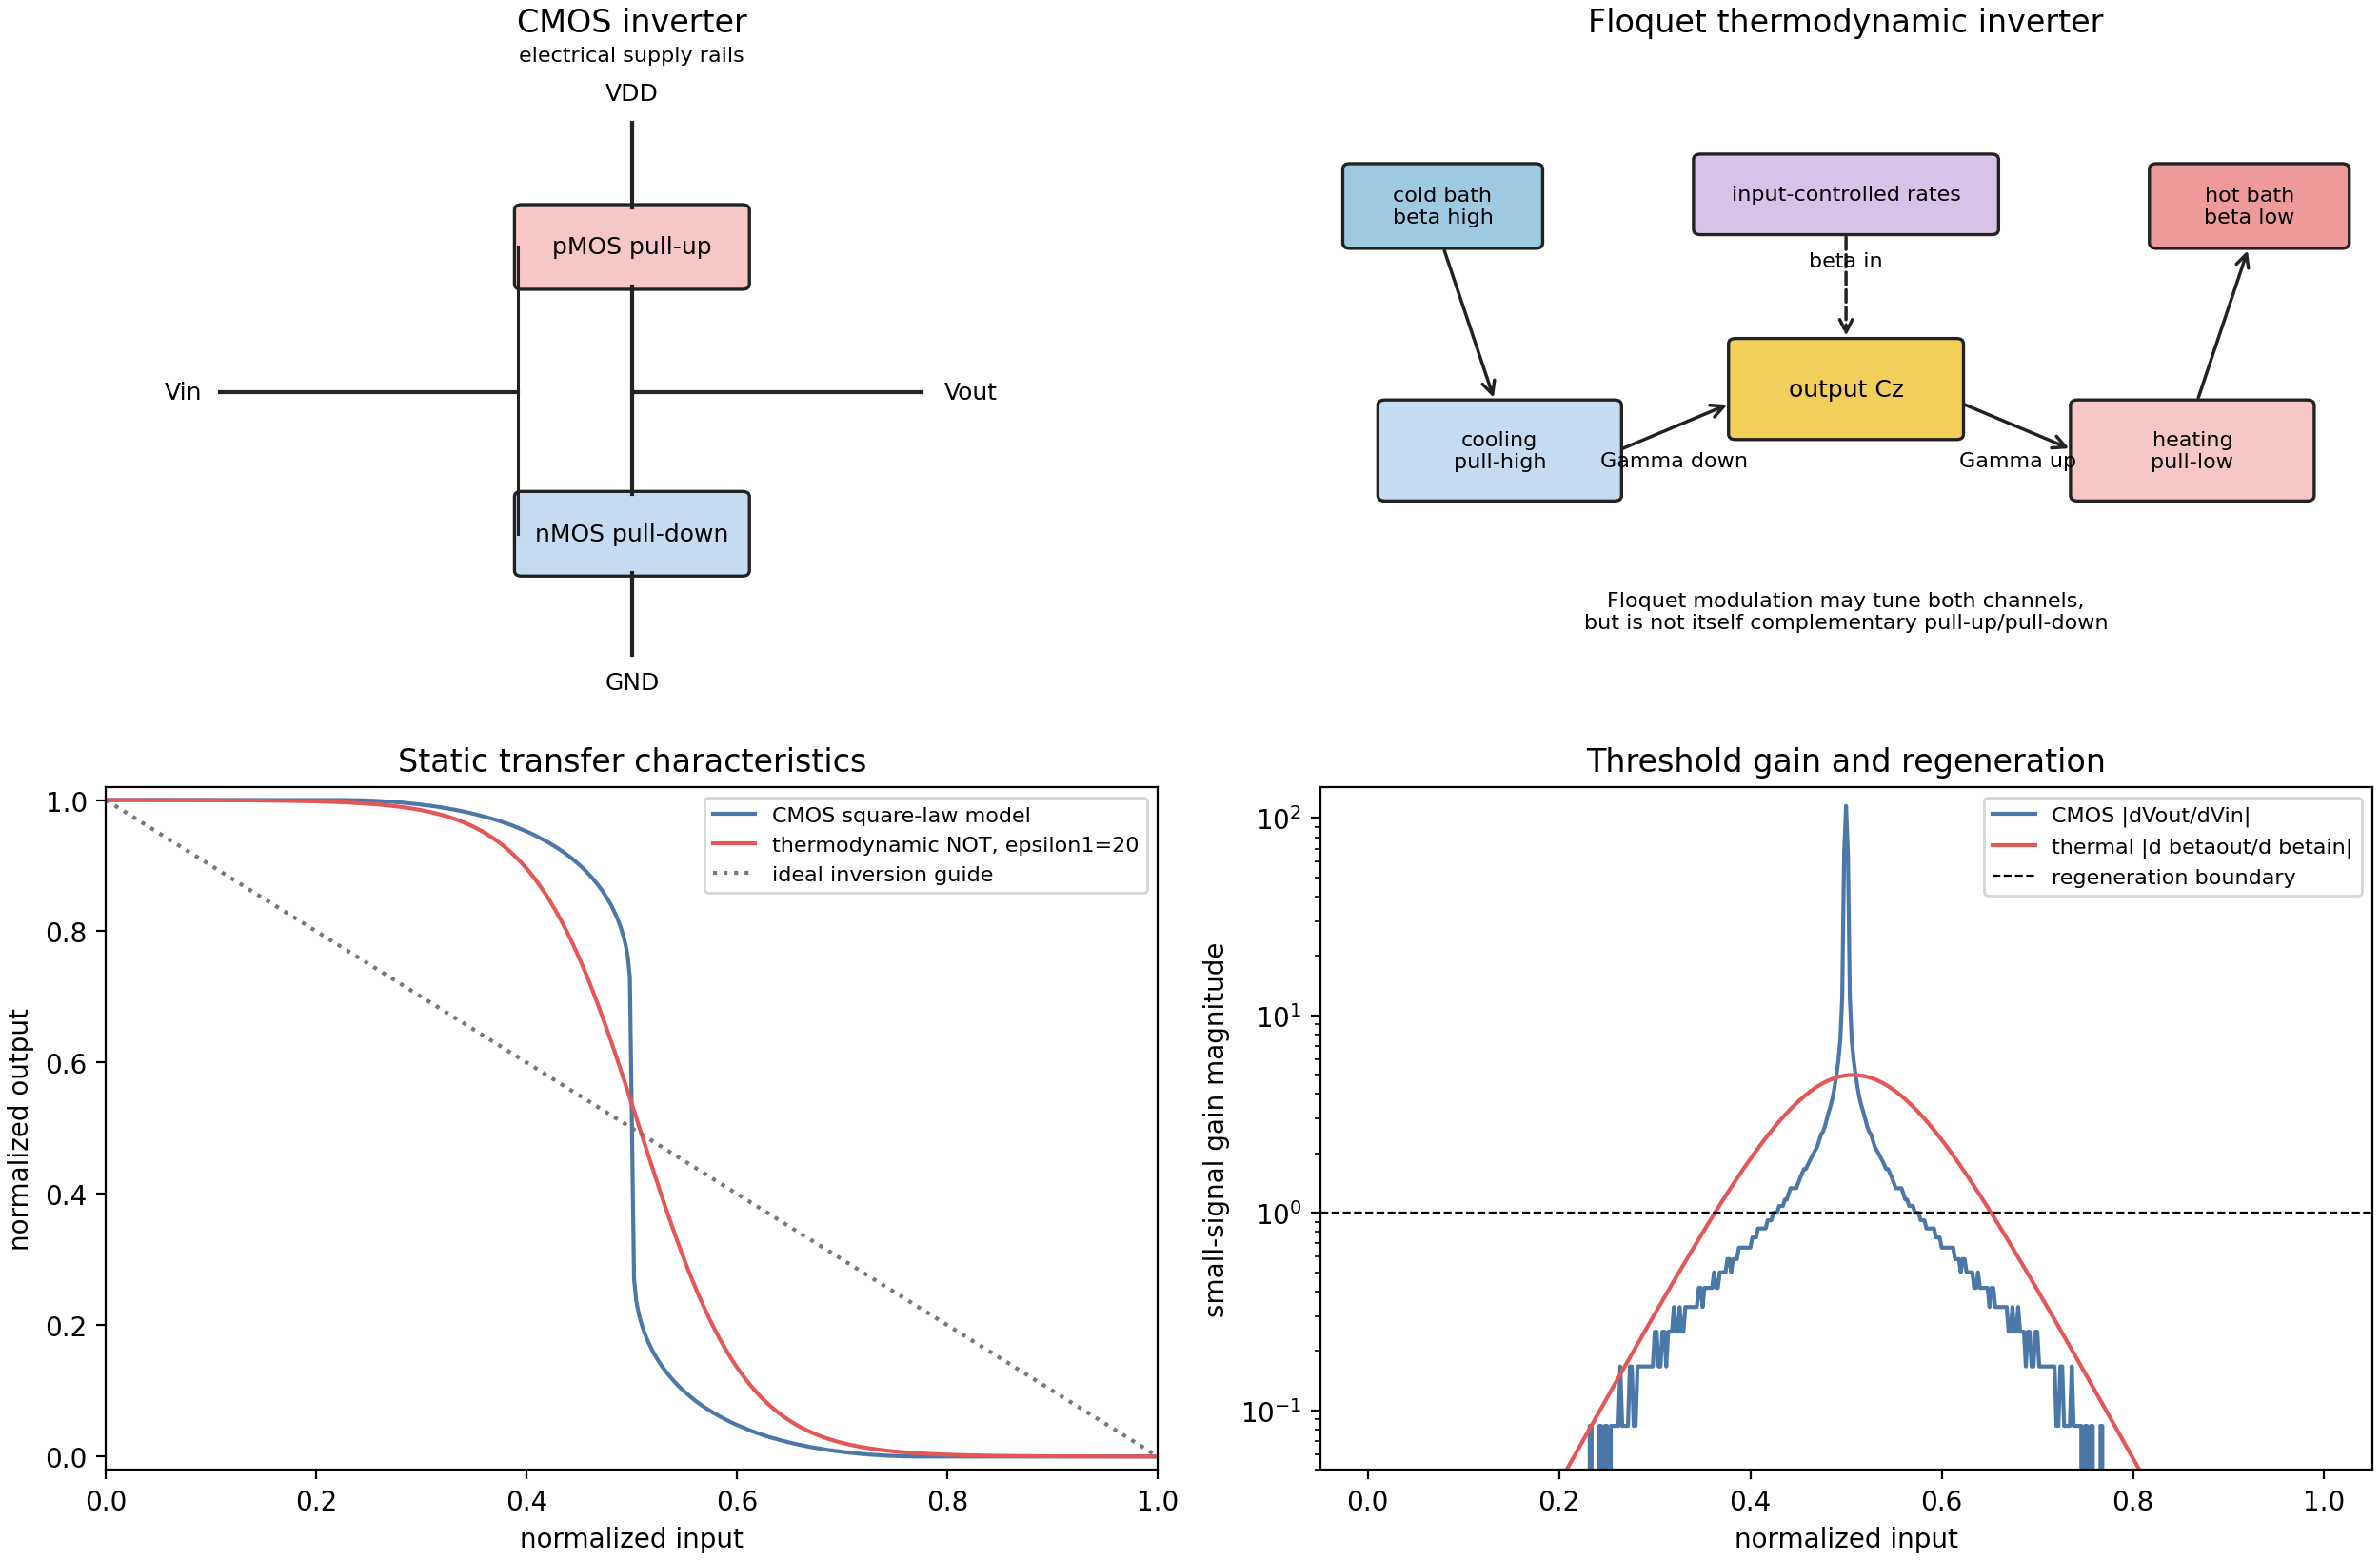
\includegraphics[width=0.98\linewidth]{cmos_floquet_inverter_comparison.png}
\caption{CMOS and thermodynamic-inverter comparison generated from code.
Top: complementary electrical pull-up/pull-down and the corresponding
cold-rail cooling / hot-rail heating architecture.  Bottom: normalized
transfer curves and small-signal gain.  The thermodynamic NOT has a
regenerative $G>1$ region, but the present Floquet buffer is a tunable
spectral stage rather than a complete complementary inverter.}
\label{fig:cmos-floquet-comparison}
\end{figure}

\begin{table}[H]\centering\small
\caption{CMOS dictionary and the limits of the analogy.}
\label{tab:cmos-thermal-dictionary}
\begin{tabularx}{\textwidth}{@{}l X X@{}}
\toprule
CMOS quantity & Thermodynamic counterpart & Important limitation \\
\midrule
$V_{\rm in}$ & Input bath inverse temperature or virtual temperature & Temperature is not an instantaneous node voltage. \\
$V_{\rm out}$ & Output $\beta_{\rm out}$, polarization, or decoded population & Usually inferred statistically from repeated measurements. \\
$V_{DD}$/ground & Cold high-$\beta$ / hot low-$\beta$ logical rails & Rails are reservoirs with heat and entropy currents. \\
pMOS/nMOS & Cooling pull-high / heating pull-low dissipative channels & Hamiltonian couplings are generally bidirectional, not ideal unilateral switches. \\
Voltage gain & $|\mathrm{d}\beta_{\rm out}/\mathrm{d}\beta_{\rm in}|$ or normalized $G$ & Trace-distance preservation is a separate quantum-channel metric. \\
Noise margin & Distance from the thermal decoding threshold & Depends on bath fluctuations, finite heat capacity, and readout statistics. \\
Fan-out & One decoded thermal output biasing later gates & Arbitrary quantum states cannot be copied; practical cascading is classical or dissipative. \\
Supply power & Steady heat currents plus any Floquet work & Must include entropy production, reset, and control-line losses. \\
\bottomrule
\end{tabularx}
\end{table}

The correct engineering statement is therefore narrower than
``Floquet buffer equals CMOS inverter.''  Both can isolate a logical node,
shape a sigmoidal inversion curve, and improve noise margin through a
regenerative region.  CMOS already integrates complementary restoration,
directional gain, stiff rails, and mature fan-out.  The current Floquet
buffer supplies spectral isolation and tunability; it becomes genuinely
CMOS-like only when embedded in a two-channel thermal architecture whose
opposing rates restore both logical rails and whose output remains stable
under a specified downstream load.

\section{Robustness programme and outlook}
\label{sec:robustness}
The remaining scientific task is to map the region where the buffered
thermodynamic NOT stays correct \emph{and} well separated. The parameter
vector is
$\theta=(\alpha,\omega_c,s,\tau_{\mathrm{mem}},\Delta t,A,\Omega,
g_{SF},\epsilon_F,t_f)$, and the robust region enforces a margin,
\begin{equation}
\calR_{\mathrm{robust}}(m_0)=\{\theta:\calA_{\mathrm{NOT}}(\theta)=1,\;
m(\theta)>m_0\},
\end{equation}
the central comparison being
$\calR_{\mathrm{robust}}^{\mathrm{buffered}}(m_0)$ versus
$\calR_{\mathrm{robust}}^{\mathrm{direct}}(m_0)$. Each point is classified
as fail ($\calA<1$), fragile pass ($\calA=1$, $m<m_0$), or robust pass
($\calA=1$, $m\ge m_0$). A first GKSL surrogate sweep ($80$ points,
$m_0=0.05$) gave $68$ robust passes, $0$ fragile, $12$ fail
(Figs.~\ref{fig:robmap}--\ref{fig:rob3d}); however the best
buffered--minus--direct margin gain was only $4.02\times10^{-5}$, so in
this surrogate the buffer preserves the truth table without yet enlarging
the margin.  The reduced output-stage HEOM sweep now establishes a
positive drive-specific distinguishability increment at all $243$ matched
points, but it does not propagate the full three-qubit Boolean gate.
Therefore enlargement of the \emph{full-gate} robust region still requires
the PT--MPO/TEMPO or a full-machine HEOM backend.

\begin{figure}[H]\centering
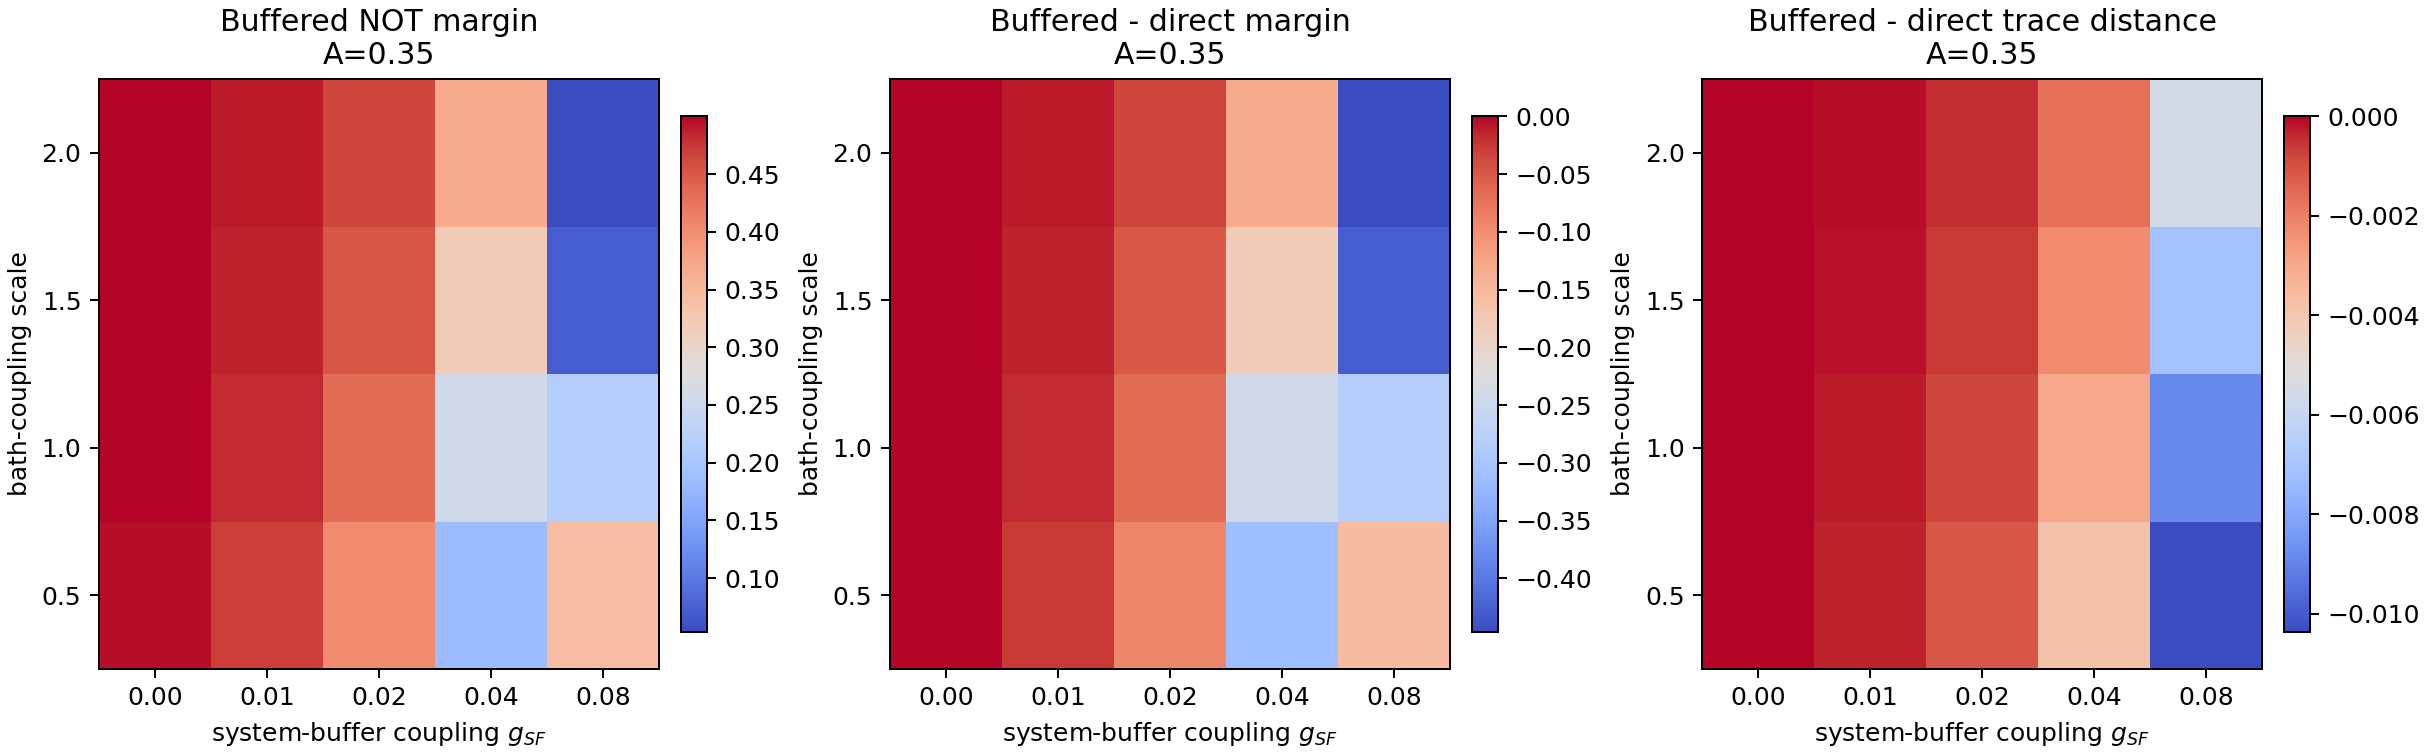
\includegraphics[width=0.92\linewidth]{robustness_phase_maps.png}
\caption{GKSL robustness phase maps at the largest drive amplitude:
buffered margin, buffered$-$direct margin, and trace--distance gain over
system--buffer and bath--coupling scales.}
\label{fig:robmap}
\end{figure}
\begin{figure}[H]\centering
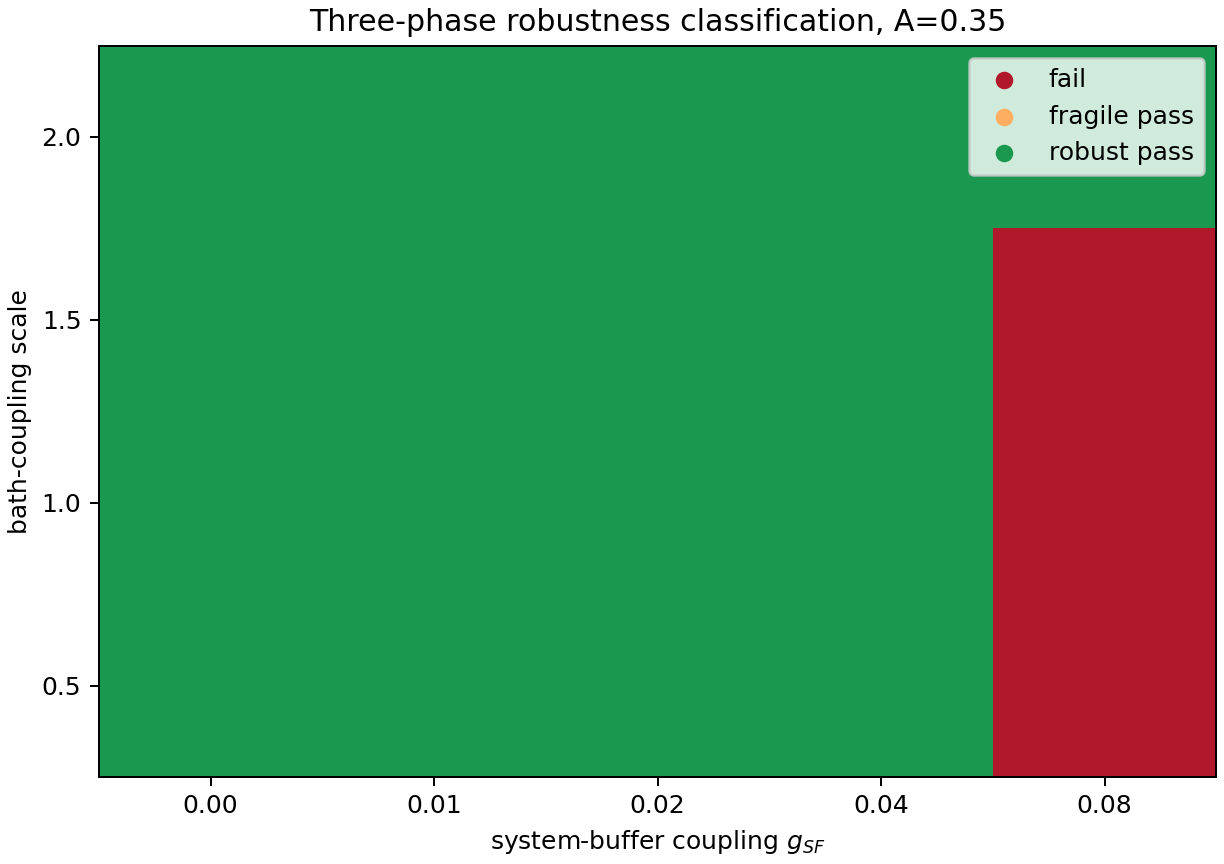
\includegraphics[width=0.68\linewidth]{robustness_three_phase_classification.png}
\caption{Three--phase classification (robust pass / fragile / fail),
analogous to CMOS noise--margin analysis.}
\label{fig:rob3class}
\end{figure}
\begin{figure}[H]\centering
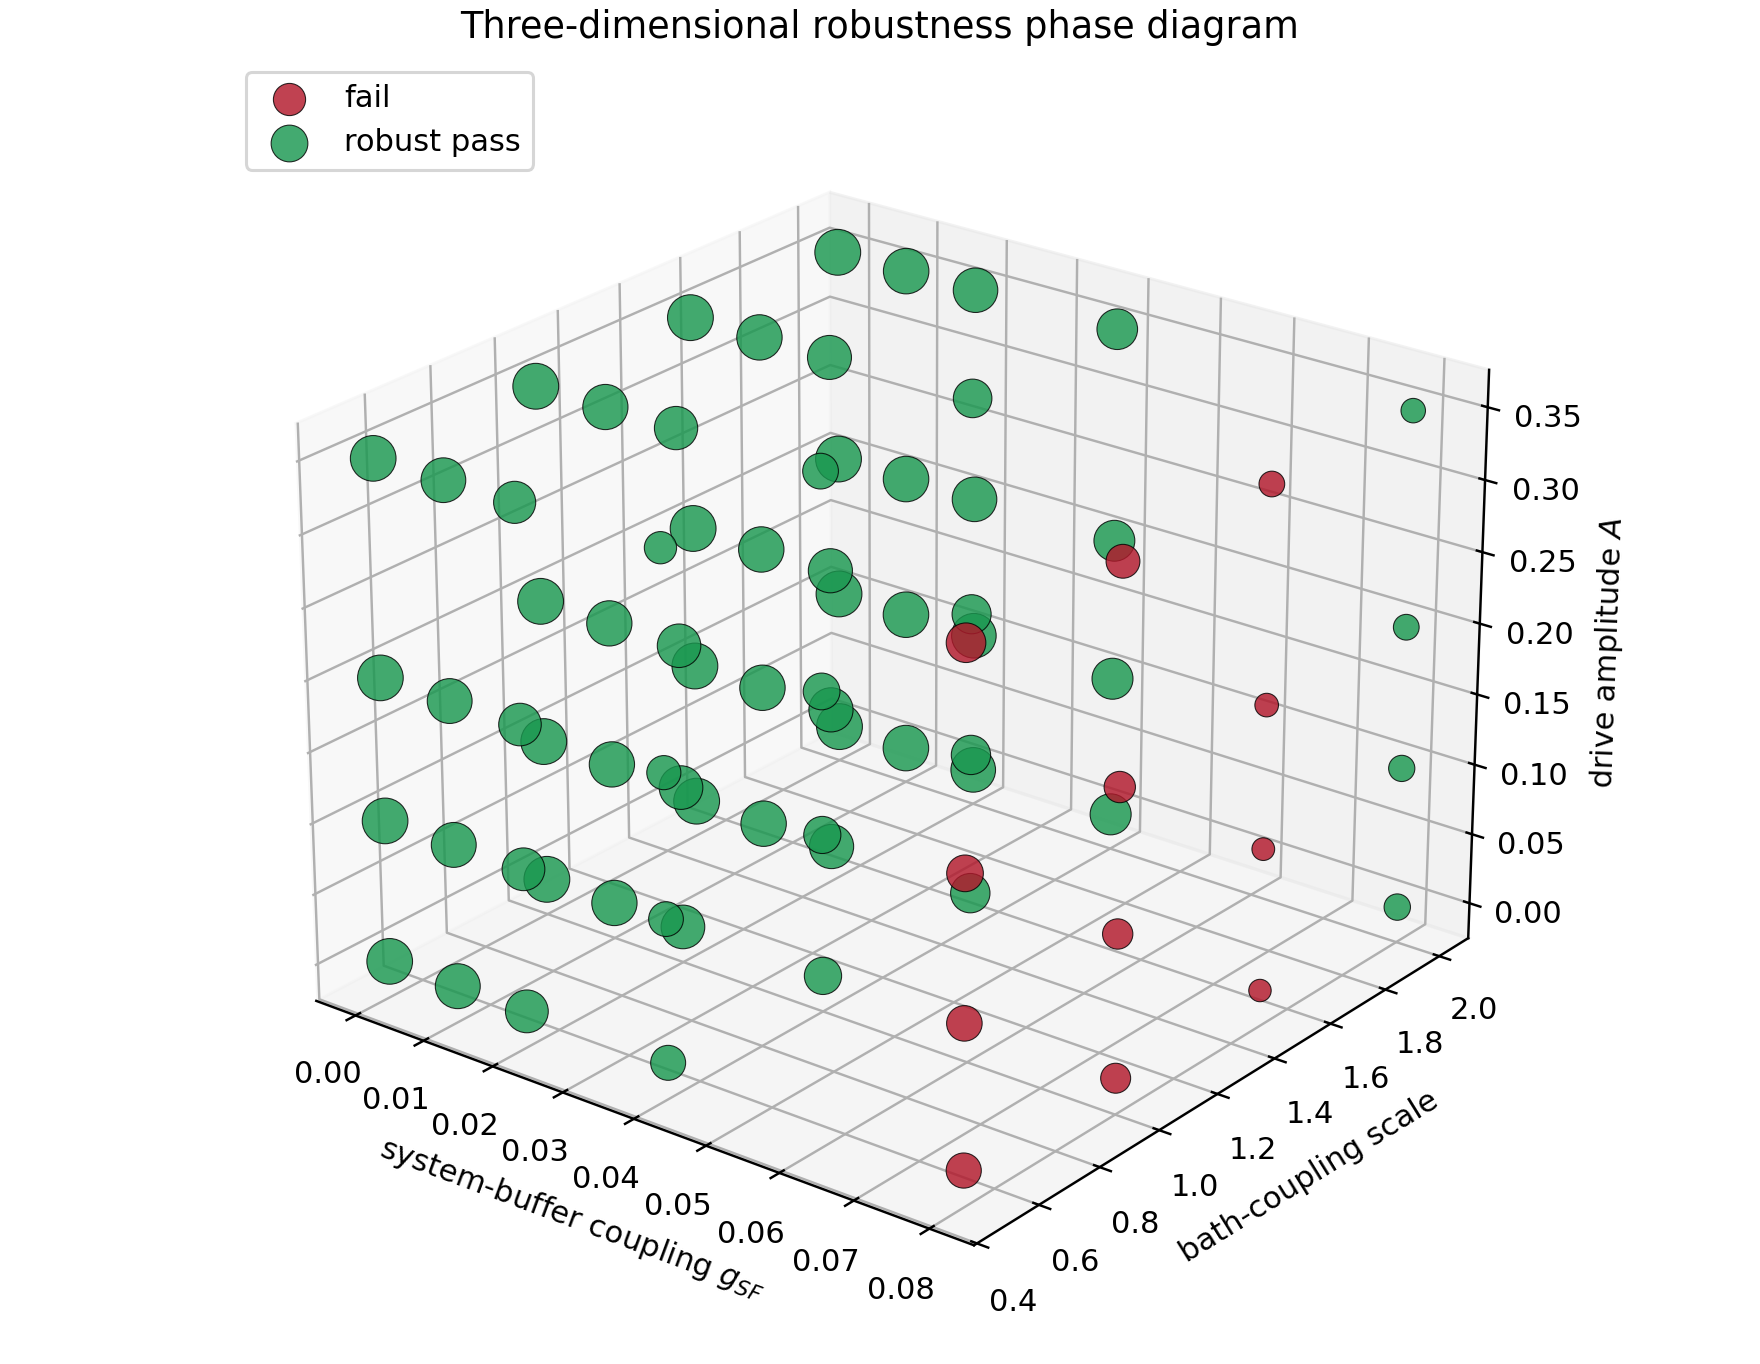
\includegraphics[width=0.66\linewidth]{robustness_phase_3d.png}
\caption{Three--dimensional robustness phase diagram over drive amplitude,
bath--coupling scale, and system--buffer coupling; marker size scales with
the buffered decoding margin.}
\label{fig:rob3d}
\end{figure}

\paragraph{Validation required for a journal--grade claim.} The present
output-stage HEOM work supplies hierarchy convergence, an independent
structured-bath benchmark, disorder sampling, energy bookkeeping, and a
trace-distance-backflow diagnostic.  Before asserting that the buffer
enlarges the \emph{full-gate} robust region under genuine memory, the
programme must still add: (i) a weak--coupling cross--check that PT--MPO
reproduces the GKSL limit; (ii) a full-gate PT--MPO convergence surface
$(\Delta t,\tau_{\mathrm{mem}},\epsilon_{\mathrm{SVD}})\mapsto
(\calA_{\mathrm{NOT}},m,\max_t\delta_{\mathrm{tr}},\max_t\delta_{\mathrm{herm}})$;
(iii) converged MPS/TTN propagation of the complete gate and reservoirs;
(iv) threshold cross--validation on held-out bath parameters; and (v) a
full-device strong-coupling audit including heat, interaction energy,
reset, and drive-line losses. A robust claim requires the same truth table
and the same sign of the buffer advantage to survive refinement of these
controls.

\paragraph{Outlook.} The staged evidence is: an analytic baseline that
reconstructs the NOT mechanism; a three--qubit GKSL surrogate that passes
the direct and buffered truth tables; and a corrected PT--MPO/TEMPO
structured--bath backend that also passes a calibrated truth table but with
a small buffered margin; and a converged reduced HEOM output model whose
buffer and drive contributions are now separated quantitatively. The
project has thus entered the full-gate robustness--mapping stage.
Output-stage drive work has been audited in the stated convention, while
full-device heat, entropy, reset, and wall-plug claims remain provisional.
The rigorous driven--dissipative
foundation for that programme --- the periodic GKSL generator, the
chain/MPS treatment, and the work--distinguishability conjecture --- is the
subject of Part~\ref{part:abhishek}.

% #####################################################################
% Abhishek's part is inserted verbatim below (kept intact).
% #####################################################################
\clearpage

\part{Abhishek: Periodically Driven Open‑System Logic Gates}
\label{part:abhishek}

\section{Introduction}
\subsection{What is thermodynamic computing?}
Thermodynamic computing \cite{Conte2019} proposes that the natural relaxation of a physical system coupled to heat baths can be harnessed to perform computation. In the quantum regime, autonomous thermal machines composed of a few interacting qubits can act as ``thermodynamic neurons'': logical inputs are encoded in the temperatures of finite‑size heat baths, and the logical output is read from the temperature of an auxiliary output bath once the system has settled into a nonequilibrium steady state (NESS) \cite{LipkaBartosik2024, Meier2025}. The key appeal is that such devices operate without an external clock: computation is driven entirely by the flow of heat from hot to cold reservoirs.

\subsection{Why add periodic driving?}
All existing quantum thermodynamic neurons are \emph{autonomous}, i.e., their Hamiltonians are time‑independent. In this note we ask a natural question: can one improve the speed or accuracy of a thermodynamic neuron by adding a periodic driving field? This is a form of \emph{Floquet engineering}: a periodically driven auxiliary system (the \emph{Floquet buffer}) is inserted between the logical qubits and the physical baths. The buffer acts as a tunable effective environment whose spectral density can be shaped by the drive.

The price is twofold. First, the device is no longer autonomous; it requires a classical clock to maintain the drive and to read out the result stroboscopically. Second, an external work input is needed to power the drive. Nevertheless, the resulting architecture---a \emph{periodically driven dissipative logic gate}---is an interesting candidate for low‑energy computation.

\subsection{Scope and structure of this note}
This note is written as a self‑contained pedagogical resource for a collaborative project involving a theoretical physicist, a mathematician working on tensor networks, and an MSc student with a background in engineering and coding. We assume familiarity with basic quantum mechanics (Hilbert spaces, operators, partial trace, von Neumann equation) and statistical mechanics (canonical ensemble, partition function). All more advanced concepts (GKSL equation, Floquet theory, chain mapping of baths, matrix‑product states) are reviewed in the main text or in the appendices.

The note is organised as follows.
\begin{itemize}
    \item Section~\ref{sec:background} provides concise reviews of the GKSL master equation, Floquet theory, the chain representation of bosonic baths, matrix‑product states (MPS), and the trace distance as a distinguishability measure.
    \item Section~\ref{sec:architecture} describes the Floquet‑buffer architecture in detail.
    \item Section~\ref{sec:weak} states and proves a theorem (Proposition~\ref{prop:periodic}) that in a certain weak‑coupling limit the logical qubits obey a time‑periodic GKSL equation.
    \item Section~\ref{sec:nonMarkovian} explains how to go beyond weak coupling using chain mapping and MPS, and how to extract energy currents and work without exponentially large bond dimensions.
    \item Section~\ref{sec:conjecture} proposes a conjectured work–distinguishability tradeoff.
    \item Section~\ref{sec:numerics} outlines a staged numerical programme.
    \item The appendices contain additional technical details.
\end{itemize}

\section{Background material}\label{sec:background}
Here we collect, in a deliberately compact form, the mathematical tools that are essential for the rest of the note. The reader may skip this section on first reading and return as needed.

\subsection{GKSL (Lindblad) master equation}\label{sec:GKSL}
A Markovian open quantum system is described by a density matrix $\rho$ evolving under the GKSL (Gorini‑Kossakowski‑Sudarshan‑Lindblad) equation:
\begin{equation}\label{eq:GKSL_general}
\dot\rho = -\ii[H,\rho] + \sum_k \gamma_k \Big( L_k \rho L_k^\dagger - \tfrac12 \{ L_k^\dagger L_k, \rho \} \Big),
\end{equation}
where $H$ is the effective system Hamiltonian, $L_k$ are jump operators, and $\gamma_k\ge0$ are positive rates. The generator is trace‑preserving and completely positive. If the rates satisfy local detailed balance with respect to a heat bath at inverse temperature $\beta$, the system relaxes to a Gibbs state $\rho_\beta\propto\ee^{-\beta H}$ (when there is only one bath) or to a NESS when several baths are present.

\subsection{Floquet theory and Floquet‑Lindblad equation}\label{sec:Floquet}
A periodically driven system has a Hamiltonian $H(t)=H(t+T)$ with $T=2\pi/\Omega$. The time‑evolution operator can be written in terms of Floquet modes $\ket{\phi_n(t)}$ and quasi‑energies $\epsilon_n$:
\begin{equation}
U(t) = \sum_n \ee^{-\ii \epsilon_n t} \ket{\phi_n(t)}\bra{\phi_n(0)},
\end{equation}
where $\ket{\phi_n(t+T)}=\ket{\phi_n(t)}$ and $\epsilon_n\in[-\Omega/2,\Omega/2)$.

When the system is open and weakly coupled to one or more baths, a Floquet‑Lindblad equation can be derived \cite{Kurizki2015, Brandner2016}. The generator becomes time‑periodic:
\begin{equation}
\dot\rho(t) = \mathcal{L}(t)\rho(t),\qquad \mathcal{L}(t+T)=\mathcal{L}(t).
\end{equation}
The jump operators are expressed in the Floquet basis, and the rates depend on the Fourier components of the bath correlation functions at frequencies shifted by multiples of $\Omega$. A crucial feature is the appearance of sidebands: transitions can occur at energies $\epsilon_m-\epsilon_n + q\Omega$, $q\in\bbZ$, which allows the system to absorb or emit quanta of the drive while exchanging energy with the baths.

\subsection{Chain mapping of bosonic baths}\label{sec:chain}
A heat bath is usually modelled as a collection of independent harmonic oscillators:
\begin{equation}
H_B = \int_0^\infty \d\omega\, \omega\, a_\omega^\dagger a_\omega,
\end{equation}
coupled to the system by $H_{SB} = A\otimes \int \d\omega\, \sqrt{J(\omega)}(a_\omega+a_\omega^\dagger)$, where $J(\omega)$ is the spectral density. For numerical purposes it is convenient to map this continuum model to a semi‑infinite one‑dimensional chain with nearest‑neighbour hopping \cite{Chin2010, Prior2010}. The transformation uses a sequence of orthogonal polynomials (e.g., Lanczos or Chebyshev) determined by $J(\omega)$. After the mapping, the Hamiltonian becomes
\begin{equation}\label{eq:chainH}
H_{\text{chain}} = \sum_{k=1}^\infty \omega_k a_k^\dagger a_k + \sum_{k=1}^\infty t_k (a_k^\dagger a_{k+1} + a_{k+1}^\dagger a_k),
\end{equation}
where $a_k$ ($k\ge1$) are new bosonic operators, and the system couples only to the first site: $H_{SB} \propto A\otimes (a_1 + a_1^\dagger)$. The parameters $\omega_k$ and $t_k$ are determined recursively from the spectral density. For an Ohmic bath $J(\omega)\propto\omega$ with a suitable cutoff, the coefficients $t_k$ decay rapidly with $k$, so that a truncation to a finite chain of length $N$ (typically $N\sim 100-200$) gives converged results for the reduced system dynamics.

\subsection{Matrix‑product states (MPS) and the TDVP}\label{sec:MPS}
A one‑dimensional quantum lattice system (such as the chain‑mapped bath) can be efficiently represented by a matrix‑product state:
\begin{equation}
\ket{\psi} = \sum_{\{s_i\}} C^{s_1} A^{s_2} \cdots A^{s_N} \ket{s_1 s_2 \dots s_N},
\end{equation}
where $C$ and $A^{s_i}$ are matrices, and the bond dimension $\chi$ controls the amount of entanglement that can be captured. The time‑dependent variational principle (TDVP) or Trotter‑Suzuki decompositions allow one to evolve the MPS in real time under a Hamiltonian $H(t)$. The computational cost scales as $O(N\chi^3 d^2)$ per time step, where $d$ is the local Hilbert space dimension.

For the chain‑mapped bath at moderate temperature, the entanglement entropy between the system and the first few chain sites saturates at a finite value. Consequently, the required bond dimension $\chi$ does not grow with the chain length $N$; values of $\chi\approx 30$–$50$ are typical for converged simulations.

\subsection{Trace distance as a distinguishability measure}\label{sec:trace}
The trace distance between two density matrices $\rho$ and $\sigma$ is
\begin{equation}
D(\rho,\sigma) = \tfrac12 \norm{\rho-\sigma}_1,
\end{equation}
where $\norm{A}_1=\Tr\sqrt{A^\dagger A}$. It satisfies $0\le D(\rho,\sigma)\le 1$ and is a metric on the space of states. Operationally, $D(\rho,\sigma)$ is equal to the maximum success probability of distinguishing $\rho$ from $\sigma$ with a single measurement. We will use it to quantify the logical distinguishability: for a binary logic gate, the two possible output states $\rho_{\text{out}}^{(0)}$ and $\rho_{\text{out}}^{(1)}$ are perfectly distinguishable when $D=1$, and completely indistinguishable when $D=0$.

\section{Architecture of the Floquet‑buffered logic gate}\label{sec:architecture}
The physical device is sketched in Fig.~\ref{fig:schematic}. It consists of:
\begin{itemize}
    \item \textbf{Logical qubits} $\calS$, described by a time‑independent Hamiltonian $H_S$. For concreteness, in the numerical programme we will use three qubits forming a NOR gate as in \cite{LipkaBartosik2024}.
    \item \textbf{Floquet buffer} $\calB_F$, a finite quantum system with a time‑periodic Hamiltonian $H_{\text{buf}}(t)=H_{\text{buf}}(t+T)$, $T=2\pi/\Omega$. The buffer could be, for example, a harmonic oscillator with a modulated frequency or a driven two‑level system.
    \item \textbf{System‑buffer coupling} $H_{S\text{buf}}$, assumed time‑independent and, for the weak‑coupling theorem, weak.
    \item \textbf{Thermal baths}, each at a different temperature $T_\alpha$, coupled only to the buffer via $H_{\text{buf},B_\alpha}$.
\end{itemize}

The logical input is encoded in the temperatures $\{T_\alpha\}$ of the baths, exactly as in the autonomous thermodynamic neuron. The output, however, is not read from an auxiliary bath; instead, we measure an observable of the output qubit stroboscopically at times $t_n=nT$, after a periodic steady state has been reached. This is a deliberate departure from strict autonomy: the device requires an external clock to synchronise the drive and the readout.

The reasons for this choice are twofold. First, in the autonomous model the output bath temperature depends on the qubit‑bath coupling, which is absent in our architecture (the qubits couple only to the buffer). Second, stroboscopic readout is natural in Floquet systems and is used in many quantum computing platforms.

Because we accept a clock, the thermodynamics of the device is that of a periodically driven open system. The relevant energetic quantities are the cycle‑averaged work $\overline{W}$ provided by the drive and the cycle‑averaged heat currents $\overline{J}_\alpha$ into the baths.

\begin{figure}[h]
\centering
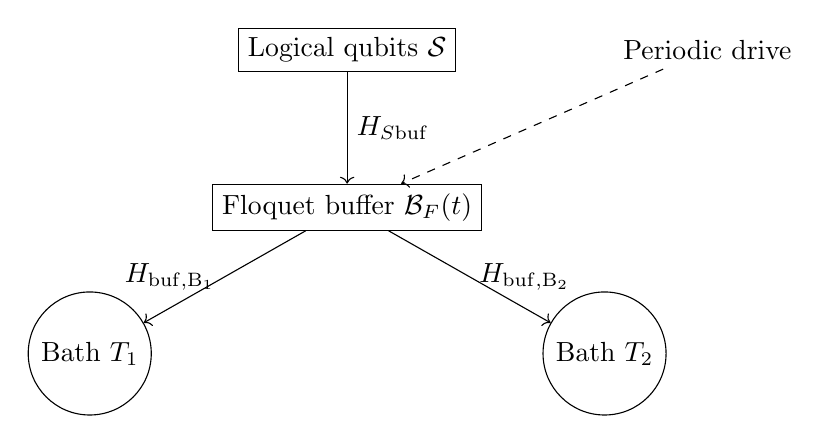
\begin{tikzpicture}[node distance=2cm]
\node[draw, rectangle] (qubits) {Logical qubits $\calS$};
\node[draw, rectangle, below of=qubits] (buffer) {Floquet buffer $\calB_F(t)$};
\node[draw, circle, below left=1cm and 1cm of buffer] (bath1) {Bath $T_1$};
\node[draw, circle, below right=1cm and 1cm of buffer] (bath2) {Bath $T_2$};
\draw[->] (qubits) -- (buffer) node[midway, right] {$H_{S\rm buf}$};
\draw[->] (buffer) -- (bath1) node[midway, left] {$H_{\rm buf, B_1}$};
\draw[->] (buffer) -- (bath2) node[midway, right] {$H_{\rm buf, B_2}$};
\node[right=2cm of qubits] (drive) {Periodic drive};
\draw[->,dashed] (drive) -- (buffer);
\end{tikzpicture}
\caption{Periodically driven logic gate with Floquet buffer. The logical qubits interact only with the driven buffer; the buffer couples to thermal reservoirs. The device is not fully autonomous: a classical clock synchronises the drive and the stroboscopic readout.}
\label{fig:schematic}
\end{figure}

\section{Weak‑coupling regime: periodic GKSL generator}\label{sec:weak}
Under certain idealised conditions, one can eliminate the buffer and the baths and obtain a closed description of the logical qubits alone.

\subsection{Assumptions}
We impose:
\begin{enumerate}[label=(A\arabic*),leftmargin=*]
    \item \textbf{Weak buffer‑bath coupling.} The interactions $H_{\text{buf},B_\alpha}$ are sufficiently weak that the buffer, when decoupled from $\calS$, relaxes to a unique periodic steady state $\rho_{\text{buf},ss}(t)$ under the Floquet‑Lindblad equation. The generator of this buffer‑only dynamics is $\mathcal{L}_{\text{buf}}(t)$.
    \item \textbf{Exponential decay of buffer correlations.} In that periodic steady state, the two‑time correlation functions $\langle B_i(t)B_j(t-\tau)\rangle$ decay to zero on a characteristic time scale $\tau_c$. More precisely, there exists $\tau_c$ such that $|C_{ij}(t,\tau)|<\varepsilon$ for $\tau>\tau_c$ for any chosen tolerance $\varepsilon$.
    \item \textbf{Weak system‑buffer coupling and time‑scale separation.} The coupling $H_{S\text{buf}}$ is much weaker than the buffer’s internal relaxation scale, and the logical qubits evolve slowly compared to $\tau_c$. This allows us to apply the Born–Markov approximation.
    \item \textbf{Secular approximation.} The Bohr frequencies (transition frequencies) of $H_S$ are non‑degenerate and well separated compared to the relaxation rates induced by the buffer.
\end{enumerate}

\subsection{Periodic GKSL generator}
\begin{proposition}\label{prop:periodic}
Under Assumptions (A1)–(A4), there exists a time‑periodic generator $\mathcal{L}_{\text{eff}}(t)$ of the form
\begin{equation}
\mathcal{L}_{\text{eff}}(t)\rho = -\ii[H_S + H_{LS}(t), \rho] + \sum_k \Gamma_k(t) \Big( L_k(t) \rho L_k^\dagger(t) - \tfrac12\{ L_k^\dagger(t)L_k(t),\rho \} \Big),
\end{equation}
with $\mathcal{L}_{\text{eff}}(t+T)=\mathcal{L}_{\text{eff}}(t)$, such that the reduced state of the logical qubits obeys
\begin{equation}\label{eq:periodic_dyn}
\dot\rho_S(t) = \mathcal{L}_{\text{eff}}(t)\rho_S(t).
\end{equation}
The jump operators $L_k(t)$ and rates $\Gamma_k(t)$ are obtained from the Fourier transforms of the buffer correlation functions evaluated at the Bohr frequencies of $H_S$, including sideband shifts by multiples of $\Omega$.
\end{proposition}

\paragraph{Proof sketch.}
The derivation follows the standard Floquet–Born–Markov approach \cite{Kurizki2015}. One starts from the Nakajima–Zwanzig equation with the buffer acting as a structured environment. The memory kernel is of second order in $H_{S\text{buf}}$. Because of (A2) the kernel decays on the time scale $\tau_c$, and because of (A3) the system density matrix changes slowly on that scale; we can therefore make the Markov approximation and replace the memory integral by a time‑local superoperator. The time dependence of this superoperator is inherited from the periodic buffer steady state. The secular approximation (A4) diagonalises the dynamics in the eigenbasis of $H_S$, yielding the GKSL form with time‑periodic coefficients.

\paragraph{Practical limitations.}
The assumptions are strong. In particular, the weak‑coupling condition (A3) may be hard to satisfy simultaneously with (A1) because weak buffer‑bath coupling implies a long buffer correlation time, whereas a Markovian elimination requires the buffer correlations to decay fast \emph{relative to the qubit dynamics}. Therefore Proposition~\ref{prop:periodic} should be seen as identifying a parameter window in which a simple theoretical description exists, not as a statement about generic parameters.

A second issue is the dynamic Lamb shift. The Floquet buffer will induce time‑dependent shifts $H_{LS}(t)$ in the qubit energy levels. The autonomous thermodynamic NOT gate relies on a precise resonance condition $\omega_W = \omega_X + \omega_Y$ among three qubit frequencies. The Floquet‑induced Lamb shift will generically detune this resonance and destroy the logical operation. To mitigate this, we must actively adjust the bare qubit frequencies as functions of the drive amplitude, a procedure that is realistic in circuit‑QED architectures but constitutes an additional control overhead.

For all these reasons, the main numerical programme of this project targets the regime \emph{outside} the validity of Proposition~\ref{prop:periodic}, where no simple Lindbladian exists. Nevertheless, the weak‑coupling analysis is a useful conceptual starting point.

\section{Non‑Markovian regime: chain mapping and MPS}\label{sec:nonMarkovian}
To treat arbitrary coupling strengths and memory effects, we simulate the full system‑buffer‑baths compound as a closed many‑body quantum system. We employ two established techniques: chain mapping of the baths (Sec.~\ref{sec:chain}) and matrix‑product state evolution (Sec.~\ref{sec:MPS}).

\subsection{Chain‑mapped Hamiltonian}
Starting from the original bath model with a continuum of harmonic oscillators and a given spectral density $J(\omega)$, we apply a unitary transformation (Lanczos or orthogonal‑polynomial mapping) that yields the chain Hamiltonian \eqref{eq:chainH}. The total Hamiltonian in the chain picture is
\begin{equation}\label{eq:total_chain}
\begin{aligned}
H_{\text{tot}}(t) &= H_S \;+\; H_{\text{buf}}(t) \;+\; H_{S\text{buf}} \\
&\quad + \sum_{\alpha} \Big[ \sum_{k=1}^{N_\alpha} \omega_{\alpha k} a_{\alpha k}^\dagger a_{\alpha k}
   + \sum_{k=1}^{N_\alpha-1} t_{\alpha k} (a_{\alpha k}^\dagger a_{\alpha,k+1} + \text{h.c.}) \Big] \\
&\quad + \sum_{\alpha} V_{\text{buf},\alpha} \otimes (a_{\alpha 1} + a_{\alpha 1}^\dagger).
\end{aligned}
\end{equation}
Here $N_\alpha$ is the chain length for bath $\alpha$ (chosen large enough to suppress finite‑size effects), and $V_{\text{buf},\alpha}$ is a buffer operator determined by the original buffer‑bath coupling.

This Hamiltonian describes a one‑dimensional lattice system. The logical qubits sit at the leftmost end, the buffer is next, and each bath forms a separate chain. The only interaction between qubits and baths is mediated by the buffer: the qubits couple to the buffer, and the buffer couples to the first site of each chain.

\subsection{Energy current and work}
Because the chain Hamiltonian is a closed system, thermodynamic observables can be defined exactly from the Heisenberg equations of motion.

The energy current from the logical qubits into the buffer is the time derivative of the qubit energy minus the contribution that would occur without the coupling:
\begin{equation}\label{eq:current_def}
J_{S\to\text{buf}}(t) = \ii\big\langle [H_S,\, H_{S\text{buf}}] \big\rangle.
\end{equation}
Here $\langle\cdot\rangle = \Tr(\rho_{\text{tot}}(t)\cdot)$, with $\rho_{\text{tot}}$ the state of the full chain. Because $H_S$ acts only on the qubits and $H_{S\text{buf}}$ acts on qubits and buffer, the commutator is a local operator with support on the qubits and the buffer alone. Its expectation value can therefore be computed directly from the MPS representation of the state without needing to reconstruct the full bath density matrix.

The power injected by the periodic drive is
\begin{equation}\label{eq:power_def}
P_{\text{drive}}(t) = \Big\langle \frac{\partial H_{\text{buf}}(t)}{\partial t} \Big\rangle.
\end{equation}
This is also a local observable (it acts only on the buffer). The cycle‑averaged work is
\begin{equation}
\overline{W} = \frac1T \int_0^T P_{\text{drive}}(t)\,\d t.
\end{equation}

The heat dumped into bath $\alpha$ can be obtained from the energy current flowing from the buffer into the first site of chain $\alpha$, using the buffer‑chain coupling. This current is again a local observable.

\subsection{Bond‑dimension control}
A crucial practical question is whether the MPS simulation remains tractable. For a one‑dimensional chain with nearest‑neighbour couplings, the entanglement entropy of the state follows an area law: for a gapped system it saturates to a constant; for a critical (gapless) system it grows logarithmically with the chain length. The chain‑mapped bath is gapless (the site frequencies $\omega_k$ extend to zero), but the coupling $t_k$ decays rapidly with $k$, so that only the first few tens of sites are strongly entangled with the system.

In practice, for an Ohmic spectral density with a high‑frequency cutoff and for temperatures $k_B T$ above the smallest energy scale of the chain, the bond dimension required for convergence is $\chi \approx 30$–$50$. This value does \emph{not} increase when the chain length $N$ is increased beyond the point where the first few sites have captured the relevant physics. The computational cost per time step then scales as $O(N\chi^3 d^2)$, where $d$ is the local Hilbert space dimension. For a truncated Fock space with $d=10$–$20$, this is manageable for the single‑qubit buffer prototype (Phase~3 of the numerical programme) and, with tree‑tensor‑network (TTN) enhancements, for the three‑qubit gate (Phase~4).

\section{Conjectured work–distinguishability tradeoff}\label{sec:conjecture}
In the autonomous thermodynamic neuron, logical distinguishability is intrinsically linked to the temperature difference between the baths; increasing the distinguishability requires a larger temperature gradient, which implies larger entropy production. In our driven setting, we expect a similar tradeoff: improving the logical distinguishability beyond the undriven baseline should require a positive amount of work per cycle.

Formally, let
\begin{equation}
P_{\text{dist}} = \tfrac12 \norm{ \rho_{\text{out}}^{(0)} - \rho_{\text{out}}^{(1)} }_1
\end{equation}
be the trace‑distance distinguishability of the output qubit states corresponding to the two logical inputs. Let $P_{\text{dist}}^{(0)}$ be this quantity when the buffer is undriven (i.e., the baseline autonomous gate, but with the same qubit readout), and let $\overline{W}$ be the cycle‑averaged work when the buffer is driven.

\begin{conjecture}[Work–distinguishability tradeoff]\label{conj:tradeoff}
There exists a monotonically increasing function $f$ with $f(P_{\text{dist}}^{(0)})=0$ such that
\begin{equation}
\overline{W} \ge f(P_{\text{dist}}).
\end{equation}
In particular, any enhancement $P_{\text{dist}} > P_{\text{dist}}^{(0)}$ requires $\overline{W}>0$.
\end{conjecture}

This conjecture is motivated by known thermodynamic uncertainty relations (TURs) and speed‑limit inequalities, which bound the precision of a process in terms of the entropy production or work. The precise functional form of $f$ and its dependence on the bath temperatures are open questions that the numerical programme will explore.

\section{Numerical programme}\label{sec:numerics}
We propose a staged numerical investigation, designed to proceed from controlled to more challenging regimes.

\paragraph{Phase 1: Undriven baseline.}
Reproduce the autonomous NOT gate of \cite{LipkaBartosik2024} using QuTiP. However, instead of reading the output from a bath temperature, we read it from the reduced state of a designated output qubit. This gives us the undriven distinguishability $P_{\text{dist}}^{(0)}$ and the baseline steady‑state heat currents.

\paragraph{Phase 2: Weak‑coupling Floquet buffer (QuTiP).}
Implement a single qubit coupled to a driven harmonic oscillator (the buffer), which is weakly coupled to two Ohmic baths. Use QuTiP’s Floquet‑Lindblad module to numerically verify Proposition~\ref{prop:periodic}. Explore how $P_{\text{dist}}$ and $\overline{W}$ depend on drive amplitude and frequency. Check whether the conjecture holds in this regime.

\paragraph{Phase 3: MPS chain simulation (single qubit).}
Build the chain‑mapped model of one qubit, one driven buffer, and two thermal chains using ITensor or MPSDynamics.jl. Initialise the chains in thermal states (via thermofield purification). Evolve in time until the periodic steady state is reached, then compute the energy current \eqref{eq:current_def}, the drive power \eqref{eq:power_def}, and the output qubit distinguishability. Investigate parameter regimes where the weak‑coupling assumptions fail, and test the conjecture beyond weak coupling.

\paragraph{Phase 4: Three‑qubit NOR gate.}
Extend the chain mapping to the full three‑qubit NOR gate with a single Floquet buffer. Here the bond dimension may grow; if it becomes prohibitive, we will use tree tensor networks (TTNs) or systematic truncation of the least‑coupled chain sites. The goal is to produce a phase diagram of $P_{\text{dist}}$ as a function of drive amplitude and frequency, and to test the conjecture for a practical logic gate.

All code and data will be made publicly available to facilitate reproducibility.

\section{Conclusion}
We have presented a self‑contained, pedagogical introduction to the Floquet‑buffer architecture for periodically driven logic gates. The note reviews the necessary technical background, states a rigorous theorem in the weak‑coupling limit, explains how to treat the non‑Markovian regime with chain‑mapped MPS, and formulates a clear conjecture to be tested numerically. The project is designed to utilise the complementary strengths of the collaboration: the physicist’s formal analysis, the mathematician’s tensor‑network expertise, and the student’s numerical skills. This note is the definitive starting point for the work.

\begin{appendices}
\section{Derivation of the GKSL equation from a microscopic model}
For completeness we sketch the derivation of the GKSL equation \eqref{eq:GKSL_general} from a system‑bath Hamiltonian. Consider a system $S$ coupled to a bath $B$ via $H_{SB}= \sum_i S_i\otimes B_i$. In the Born–Markov approximation, after tracing out the bath, one obtains the Redfield equation. The additional secular (rotating‑wave) approximation diagonalises the dynamics in the eigenbasis of $H_S$ and ensures complete positivity. The resulting jump operators are the eigenoperators $A(\omega)$ of the system Hamiltonian, with rates $\gamma(\omega)= \int e^{i\omega t}\langle B^\dagger(t)B(0)\rangle dt$. The detailed balance condition $\gamma(-\omega)=e^{-\beta\omega}\gamma(\omega)$ follows from the KMS condition of the bath. See \cite{Breuer2002} for a textbook treatment.

\section{Chain mapping: recurrence relations}
Given a spectral density $J(\omega)$, the chain mapping is constructed by orthogonalising the polynomials in $\omega$ with respect to the measure $J(\omega)d\omega$. The recurrence coefficients $\omega_k$ and $t_k$ are obtained from the continued fraction expansion of the bath correlation function. For the common case of an Ohmic bath with exponential cutoff, $J(\omega)= \eta\omega e^{-\omega/\omega_c}$, the coefficients can be computed analytically or numerically using the Lanczos algorithm \cite{Chin2010}.

\section{MPS representation of a thermal state}
To initialise the chain in a thermal state at temperature $T$, one uses the thermofield (purification) approach. Each physical bosonic site is doubled into an ancilla site, and the initial state is the vacuum for a set of Bogoliubov‑transformed modes. The resulting MPS bond dimension is directly related to the effective temperature; for moderate $T$, it remains small.

\section{Energy current operator: explicit form}
Equation \eqref{eq:current_def} follows from the Heisenberg equation for $H_S$:
\begin{equation}
\frac{d H_S}{dt} = \ii[ H_{\text{tot}}, H_S ] = \ii[ H_S, H_{S\text{buf}} ] + \ii[ H_S, H_S ] = \ii[ H_S, H_{S\text{buf}} ].
\end{equation}
The term $[H_S, H_S]=0$, and $H_S$ commutes with all bath and buffer‑bath Hamiltonians because it acts on a different tensor factor. Hence the energy change of the qubits is solely due to the qubit‑buffer interaction. Taking the expectation value gives the current.
\end{appendices}

\clearpage
\begin{thebibliography}{99}
\bibitem{LipkaBartosik2024} P.~Lipka--Bartosik, M.~Perarnau--Llobet, and
N.~Brunner, ``Thermodynamic computing via autonomous quantum thermal
machines,'' \emph{Sci.\ Adv.} \textbf{10}, eadm8792 (2024);
arXiv:2308.15905.

\bibitem{BrunnerVirtual2012} N.~Brunner, N.~Linden, S.~Popescu, and
P.~Skrzypczyk, ``Virtual qubits, virtual temperatures, and the
foundations of thermodynamics,'' \emph{Phys.\ Rev.\ E} \textbf{85},
051117 (2012).

\bibitem{Breuer2002} H.-P.~Breuer and F.~Petruccione, \emph{The Theory of
Open Quantum Systems}, Oxford University Press (2002).

\bibitem{Pollock2018} F.~A.~Pollock \emph{et al.}, ``Non-Markovian quantum
processes: complete framework and efficient characterization,''
\emph{Phys.\ Rev.\ A} \textbf{97}, 012127 (2018).

\bibitem{Strathearn2018} A.~Strathearn, P.~Kirton, D.~Kilda, J.~Keeling,
and B.~W.~Lovett, ``Efficient non-Markovian quantum dynamics using
time-evolving matrix product operators,'' \emph{Nat.\ Commun.} \textbf{9},
3322 (2018).

\bibitem{Grifoni1998} M.~Grifoni and P.~H\"anggi, ``Driven quantum
tunneling,'' \emph{Phys.\ Rep.} \textbf{304}, 229 (1998).

\bibitem{Conte2019} T.~Conte et al., “Thermodynamic Computing,” arXiv:1911.01968 (2019).

\bibitem{Meier2025} F.~Meier, S.~Huber, P.~Erker, and A.~Xuereb, “Autonomous Quantum Processing Unit,” arXiv:2501.15615 (2025).

\bibitem{Kurizki2015} D.~Gelbwaser-Klimovsky, W.~Niedenzu, and G.~Kurizki, “Thermodynamics of quantum systems under dynamical control,” Adv.\ At.\ Mol.\ Opt.\ Phys.\ \textbf{64}, 329 (2015).

\bibitem{Brandner2016} K.~Brandner and U.~Seifert, “Periodic thermodynamics of open quantum systems,” Phys.\ Rev.\ E \textbf{93}, 062134 (2016).

\bibitem{Chin2010} A.~W.~Chin, \'{A}.~Rivas, S.~F.~Huelga, and M.~B.~Plenio, “Exact mapping between system‑reservoir quantum models and semi‑infinite discrete chains,” J.\ Math.\ Phys.\ \textbf{51}, 092109 (2010).

\bibitem{Prior2010} J.~Prior, A.~W.~Chin, S.~F.~Huelga, and M.~B.~Plenio, “Efficient simulation of strong system‑environment interactions,” Phys.\ Rev.\ Lett.\ \textbf{105}, 050404 (2010).

\bibitem{Schollwock2011} U.~Schollw\"ock, ``The density-matrix
renormalization group in the age of matrix product states,''
\emph{Ann.\ Phys.} \textbf{326}, 96--192 (2011).

\bibitem{Orus2014} R.~Or\'us, ``A practical introduction to tensor
networks: Matrix product states and projected entangled pair states,''
\emph{Ann.\ Phys.} \textbf{349}, 117--158 (2014).

\bibitem{Gray2018} J.~Gray, ``quimb: a Python package for quantum
information and many-body calculations,'' \emph{J.\ Open Source Softw.}
\textbf{3}, 819 (2018).

\bibitem{Wolpert2022} D.~H.~Wolpert, “Stochastic thermodynamics of computation,” J.\ Stat.\ Phys.\ \textbf{187}, 10 (2022).

\bibitem{TienGordon1963} P.~K.~Tien and J.~P.~Gordon, ``Multiphoton Process Observed in the Interaction of Microwave Fields with the Tunneling between Superconductor Films,'' Phys.\ Rev.\ \textbf{129}, 647 (1963).

\bibitem{OQuPy} G.~E.~Fux, D.~Kilda, B.~W.~Lovett, and J.~Keeling, “OQuPy: A Python package to efficiently simulate non‑Markovian open quantum systems,” J.\ Chem.\ Phys.\ \textbf{161}, 124108 (2024).

\bibitem{QuTiP}
J. R. Johansson, P. D. Nation, and F. Nori,
``QuTiP: An open-source Python framework for the dynamics of open quantum systems,''
\textit{Computer Physics Communications},
vol. 183, no. 8, pp. 1760--1772, Aug. 2012.
DOI: \url{https://doi.org/10.1016/j.cpc.2012.02.021}.
\end{thebibliography}

\end{document}
